%%%%%%%%%%%%%%%%%%%%%%%%%%%%%%%%%%%%%%%%%%%%%%%%%%%
%
%  New template code for TAMU Theses and Dissertations starting Fall 2012.  
%  For more info about this template or the 
%  TAMU LaTeX User's Group, see http://www.howdy.me/.
%
%  Author: Wendy Lynn Turner 
%
%%%%%%%%%%%%%%%%%%%%%%%%%%%%%%%%%%%%%%%%%%%%%%%%%%%

\documentclass[12pt]{report}
\usepackage[letterpaper]{geometry}
\geometry{verbose,tmargin=1.25in,bmargin=1.25in,lmargin=1.4in,rmargin=1.15in}
\usepackage[doublespacing]{setspace}
\usepackage{tocloft}
\usepackage[rm, tiny,center, compact]{titlesec}
\usepackage{indentfirst}
\usepackage{etoolbox}
\usepackage{tocvsec2}
\usepackage[titletoc]{appendix}
\usepackage{appendix}
\usepackage{tamuconfig}
\usepackage{rotating}
\usepackage{amsmath,amssymb,amsthm}
\usepackage{mathrsfs}
\usepackage{xspace}

\graphicspath{{figs/}}
\DeclareGraphicsExtensions{.pdf,.eps,.jpg,.png}

\usepackage[labelformat=simple]{subfig}
\renewcommand{\thesubfigure}{(\alph{subfigure})}
\makeatletter
  \renewcommand{\p@subfigure}{\thefigure}
  \renewcommand\@biblabel[1]{#1.}
\makeatother



% Added to fix issues with pdf searching in some versions of LaTeX
%\usepackage[T1]{fontenc}\usepackage{lmodern}
%%%%%%%%%%%%%%%%%%%%%%%%%%%%%

\usepackage{hyperref}

% Hyperref setup below.  You should be able to get away with using uncommenting just the first line.
% \usepackage[hidelinks]{hyperref}

% if \usepackage[hidelinks]{hyperref} doesn't work try this.
% \usepackage{hyperref}  % Hidelinks is an option that removes link visiability.  TAMU Thesis Offices prefers to not see the links. But often doesn't work.  
% 
\hypersetup{
    colorlinks=true,
    linkcolor=black,
    citecolor=black,
    filecolor=black,
    urlcolor=black,
}
%%%%%%%  End of hyperref setup.  One of these two options should work, but my motto with hyperref is when in doubt, comment it out!
%%%%%%%%%  This hopefully fixes the problem with vertical spacing of section headings at the top of the page..
% \preto\section{%
% \ifnum\value{section}>0\addtocontents{toc}{\vskip-6pt}\fi
% }
% \preto\subsection{%
% \ifnum\value{subsection}=0\addtocontents{toc}{\vskip-6pt}\fi
% \ifnum\value{subsection}>0\addtocontents{toc}{\vskip-6pt}\fi
% } 
%%%%%%%%%%%%%%%%%%%%%%%%%%%%%%%%%%%%%%%%%%%%%%%%%%%%%%

\usepackage{rsinnet}

\begin{document}

\renewcommand{\tamumanuscripttitle}{Humanlike Bipedal Robotic Walking}
\renewcommand{\tamupapertype}{Dissertation}
\renewcommand{\tamufullname}{Ryan Wesley Sinnet}
\renewcommand{\tamudegree}{Doctor of Philosophy}
\renewcommand{\tamuchairone}{Chair Aaron Ames}
% Uncomment out the next line if you have co-chairs.  You will also need to edit the titlepage.tex file.
%\newcommand{\tamuchairtwo}{Additional Chair Name}
\renewcommand{\tamumemberone}{Reza Langari}
\newcommand{\tamumembertwo}{Richard Malak}
\newcommand{\tamumemberthree}{Dylan Shell}
\renewcommand{\tamudepthead}{Andreas Polycarpou}
\renewcommand{\tamugradmonth}{May}
\renewcommand{\tamugradyear}{2015}
\renewcommand{\tamudepartment}{Mechanical Engineering}


%%%%%%%%%%%%%%%%%%%%%%%%%%%%%%%%%%%%%%%%%%%%%%%%%%%
%
%  New template code for TAMU Theses and Dissertations starting Fall 2012.  
%  For more info about this template or the 
%  TAMU LaTeX User's Group, see http://www.howdy.me/.
%
%  Author: Wendy Lynn Turner 
%	 Version 1.0 
%  Last updated 8/5/2012
%
%%%%%%%%%%%%%%%%%%%%%%%%%%%%%%%%%%%%%%%%%%%%%%%%%%%

%%%%%%%%%%%%%%%%%%%%%%%%%%%%%% 
%% TITLE PAGE
%% The values get updated automatically.  Please do not make changes to this file other than adding/deleting committee members where necessary.
%%%%%%%%%%%%%%%%%%%%%%%%%%%%%%

\providecommand{\tabularnewline}{\\}



\begin{titlepage}
\begin{center}
  %\MakeUppercase{\tamumanuscripttitle}
  \MakeUppercase{Energy Shaping of Mechanical Systems}\\
  \MakeUppercase{via Control Lyapunov Functions}\\
  \MakeUppercase{with Applications to Bipedal Locomotion}
\vspace{4em}

A \tamupapertype

by

\MakeUppercase{\tamufullname}

\vspace{4em}

\begin{singlespace}

Submitted to the Office of Graduate and Professional Studies of \\
Texas A\&M University \\

in partial fulfillment of the requirements for the degree of \\
\end{singlespace}

\MakeUppercase{\tamudegree}
\par\end{center}
\vspace{2em}
\begin{singlespace}
\begin{tabular}{ll}
 & \tabularnewline
& \cr
% If you have Co-Chairs comment out the 'Chair of Committee' line below and uncomment the 'Co-Chairs of Committee' line.
Chair of Committee, & \tamuchairone\tabularnewline
%Co-Chairs of Committee, & \tamuchairone\tabularnewline & \tamuchairtwo\tabularnewline
Committee Members, & \tamumemberone\tabularnewline
 & \tamumembertwo\tabularnewline
 & \tamumemberthree\tabularnewline
Head of Department, & \tamudepthead\tabularnewline

\end{tabular}
\end{singlespace}
\vspace{3em}

\begin{center}
\tamugradmonth \hspace{2pt} \tamugradyear

\vspace{3em}

Major Subject: \tamudepartment \par
\vspace{3em}
Copyright \tamugradyear \hspace{.5em}\tamufullname 
\par\end{center}
\end{titlepage}
\pagebreak{}




 % This is simply a file that formats and adds your titlepage, please do not edit this unless you have a specific need.
%%%%%%%%%%%%%%%%%%%%%%%%%%%%%%%%%%%%%%%%%%%%%%%%%%%
%
%  New template code for TAMU Theses and Dissertations starting Fall 2012.  
%  For more info about this template or the 
%  TAMU LaTeX User's Group, see http://www.howdy.me/.
%
%  Author: Wendy Lynn Turner 
%	 Version 1.0 
%  Last updated 8/5/2012
%
%%%%%%%%%%%%%%%%%%%%%%%%%%%%%%%%%%%%%%%%%%%%%%%%%%%
%%%%%%%%%%%%%%%%%%%%%%%%%%%%%%%%%%%%%%%%%%%%%%%%%%%%%%%%%%%%%%%%%%%%%
%%                           ABSTRACT 
%%%%%%%%%%%%%%%%%%%%%%%%%%%%%%%%%%%%%%%%%%%%%%%%%%%%%%%%%%%%%%%%%%%%%

\chapter*{ABSTRACT}
\addcontentsline{toc}{chapter}{ABSTRACT} % Needs to be set to part, so the TOC doesnt add 'CHAPTER ' prefix in the TOC.

\pagestyle{plain} % No headers, just page numbers
\pagenumbering{roman} % Roman numerals
\setcounter{page}{2}

\indent This thesis presents a method which attempts to improve the stability
properties of periodic orbits in hybrid dynamical systems by shaping the
energy.
%
By taking advantage of conservation of energy and the existence of invariant
level sets of a conserved quantity of energy corresponding to periodic orbits,
energy shaping drives a system to a desired level set.
%
This energy shaping method is similar to existing methods but improves upon them
by utilizing control Lyapunov functions, allowing for formal results on
stability.
%
The main theoretical result, \thmref{theorem:main-theorem}, states that, given
an exponentially-stable limit cycle in a hybrid dynamical system, application of
the presented energy shaping controller results in a closed-loop system which is
exponentially stable

The method can be applied to a wide class of problems including bipedal
locomotion;
%
because the optimization problem can be formulated as a quadratic program
operating on a convex set, existing methods can be used to rapidly obtain
the optimal solution.
%
As illustrated through numerical simulations, this method turns out to be useful
in practice, taking an existing behavior which corresponds to a periodic orbit
of a hybrid system, such as steady state locomotion, and providing an
improvement in convergence properties and robustness with respect to
perturbations in initial conditions without destabilizing the behavior.
%
The method is even shown to work on complex multi-domain hybrid systems;
%
an example is provided of bipedal locomotion for a robot with non-trivial foot
contact which results in a multi-phase gait.

\pagebreak{}

%%%%%%%%%%%%%%%%%%%%%%%%%%%%%%%%%%%%%%%%%%%%%%%%%%%
%
%  New template code for TAMU Theses and Dissertations starting Fall 2012.  
%  For more info about this template or the 
%  TAMU LaTeX User's Group, see http://www.howdy.me/.
%
%  Author: Wendy Lynn Turner 
%	 Version 1.0 
%  Last updated 8/5/2012
%
%%%%%%%%%%%%%%%%%%%%%%%%%%%%%%%%%%%%%%%%%%%%%%%%%%%

%%%%%%%%%%%%%%%%%%%%%%%%%%%%%%%%%%%%%%%%%%%%%%%%%%%%%%%%%%%%%%%%%%%%%%
%%                           DEDICATION
%%%%%%%%%%%%%%%%%%%%%%%%%%%%%%%%%%%%%%%%%%%%%%%%%%%%%%%%%%%%%%%%%%%%%
\chapter*{DEDICATION}
\addcontentsline{toc}{chapter}{DEDICATION}  % Needs to be set to part, so the TOC doesnt add 'CHAPTER ' prefix in the TOC.

I dedicate this work to my grandmother Helena Sinnet.
%
She was very excited when I first entered the Ph.D. program but sadly she did
not make it through to see me graduate.


%\indent This is an optional page.

\pagebreak{}

%%%%%%%%%%%%%%%%%%%%%%%%%%%%%%%%%%%%%%%%%%%%%%%%%%%
%
%  New template code for TAMU Theses and Dissertations starting Fall 2012.  
%  For more info about this template or the 
%  TAMU LaTeX User's Group, see http://www.howdy.me/.
%
%  Author: Wendy Lynn Turner 
%	 Version 1.0 
%  Last updated 8/5/2012
%
%%%%%%%%%%%%%%%%%%%%%%%%%%%%%%%%%%%%%%%%%%%%%%%%%%%


%%%%%%%%%%%%%%%%%%%%%%%%%%%%%%%%%%%%%%%%%%%%%%%%%%%%%%%%%%%%%%%%%%%%%%
%%                           ACKNOWLEDGEMENTS
%%%%%%%%%%%%%%%%%%%%%%%%%%%%%%%%%%%%%%%%%%%%%%%%%%%%%%%%%%%%%%%%%%%%%
\chapter*{ACKNOWLEDGEMENTS}
\addcontentsline{toc}{chapter}{ACKNOWLEDGEMENTS}  % Needs to be set to part, so the TOC doesnt add 'CHAPTER ' prefix in the TOC.


%\indent 

\pagebreak{}

%%%%%%%%%%%%%%%%%%%%%%%%%%%%%%%%%%%%%%%%%%%%%%%%%%%
%
%  New template code for TAMU Theses and Dissertations starting Fall 2012.  
%  For more info about this template or the 
%  TAMU LaTeX User's Group, see http://www.howdy.me/.
%
%  Author: Wendy Lynn Turner 
%	 Version 1.0 
%  Last updated 8/5/2012
%
%%%%%%%%%%%%%%%%%%%%%%%%%%%%%%%%%%%%%%%%%%%%%%%%%%%

%%%%%%%%%%%%%%%%%%%%%%%%%%%%%%%%%%%%%%%%%%%%%%%%%%%%%%%%%%%%%%%%%%%%%%
%%                           NOMENCLATURE
%%%%%%%%%%%%%%%%%%%%%%%%%%%%%%%%%%%%%%%%%%%%%%%%%%%%%%%%%%%%%%%%%%%%%

\chapter*{NOMENCLATURE}
\addcontentsline{toc}{chapter}{NOMENCLATURE}  % Needs to be set to part, so the TOC doesnt add 'CHAPTER ' prefix in the TOC.

\begin{tabular}{ll}
B/CS  & Bryan/College Station\tabularnewline
HSUS & Humane Society of the United States\tabularnewline
P & Pressure\tabularnewline
T  & Time\tabularnewline
TVA & Tennessee Valley Authority\tabularnewline
TxDOT \hfill{}\hfill{}\hfill{}\hfill{}\hfill{}\hfill{}\hfill{}\hfill{} & \multicolumn{1}{l}{Texas Department of Transportation}\tabularnewline
\end{tabular}

\vspace{2em}

This page is optional.

\pagebreak{}


%%%%%%%%%%%%%%%%%%%%%%%%%%%%%%%%%%%%%%%%%%%%%%%%%%%
%
%  New template code for TAMU Theses and Dissertations starting Fall 2012.  
%  For more info about this template or the 
%  TAMU LaTeX User's Group, see http://www.howdy.me/.
%
%  Author: Wendy Lynn Turner 
%	 Version 1.4
%  Last updated 1/27/2013
%
%%%%%%%%%%%%%%%%%%%%%%%%%%%%%%%%%%%%%%%%%%%%%%%%%%%
%%%%%%%%%%%%%%%%%%%%%%%%%%%%%%%%%%%%%%%%%%%%%%%%%%%%%%%%%%%%%%%%%%%%%%
%%       TABLE OF CONTENTS
%%%%%%%%%%%%%%%%%%%%%%%%%%%%%%%%%%%%%%%%%%%%%%%%%%%%%%%%%%%%%%%%%%%%%
% single-space sections in Table of Contents
\renewcommand{\cftsecafterpnum}{\vskip0.5\baselineskip}
\renewcommand{\cftsubsecafterpnum}{\vskip0.5\baselineskip}
\renewcommand{\cftsubsubsecafterpnum}{\vskip0.5\baselineskip}
%%%%%%%%%%%%%%%%%%%%%%%%%%%%%%%%%%%%%%%%%%%%%%%%%%%

\phantomsection
\addcontentsline{toc}{chapter}{TABLE OF CONTENTS}  

\begin{singlespace}
\renewcommand\contentsname{\normalfont} {\centerline{TABLE OF CONTENTS}}

%\setcounter{tocdepth}{4} % This puts \subsubsection[]{×} in your List of Tables.  The default is 3.


%%%%%%%%%%%%%  Adds Page above the page number in TOC
\setlength{\cftaftertoctitleskip}{1em}
\renewcommand{\cftaftertoctitle}{%
\hfill{\normalfont {Page}\par}}



\tableofcontents

\end{singlespace}

\pagebreak{}

%%%%%%%%%%%%%%%%%%%%%%%%%%%%%%%%%%%%%%%%%%%%%%%%%%%%%%%%%%%%%%%%%%%%%%
%%                           LIST OF FIGURES
%%%%%%%%%%%%%%%%%%%%%%%%%%%%%%%%%%%%%%%%%%%%%%%%%%%%%%%%%%%%%%%%%%%%%

\phantomsection
\addcontentsline{toc}{chapter}{LIST OF FIGURES}  

\renewcommand{\cftloftitlefont}{\center\normalfont\MakeUppercase}

\setlength{\cftbeforeloftitleskip}{-12pt} %% Positions the LOF title vertically to match the chapter titles
\renewcommand{\cftafterloftitleskip}{12pt}


\renewcommand{\cftafterloftitle}{%
\\[4em]\mbox{}\hspace{2pt}FIGURE\hfill{\normalfont Page}\vskip\baselineskip}

\begingroup


\begin{center}
\begin{singlespace}
%% These values make the lof table entries appear double spaced between.
\setlength{\cftbeforechapskip}{0.4cm}
\setlength{\cftbeforesecskip}{0.30cm}
\setlength{\cftbeforesubsecskip}{0.30cm}
\setlength{\cftbeforefigskip}{0.4cm}
\setlength{\cftbeforetabskip}{0.4cm} 

\listoffigures

\end{singlespace}
\end{center}

\pagebreak{}


%%%%%%%%%%%%%%%%%%%%%%%%%%%%%%%%%%%%%%%%%%%%%%%%%%%%%%%%%%%%%%%%%%%%%%
%%                           lIST OF TABLES
%%%%%%%%%%%%%%%%%%%%%%%%%%%%%%%%%%%%%%%%%%%%%%%%%%%%%%%%%%%%%%%%%%%%%%
%
\phantomsection
\addcontentsline{toc}{chapter}{LIST OF TABLES}  

\renewcommand{\cftlottitlefont}{\center\normalfont\MakeUppercase}

\setlength{\cftbeforelottitleskip}{-12pt} %% Positions the LOT title vertically to match the chapter titles

\renewcommand{\cftafterlottitleskip}{12pt}


\renewcommand{\cftafterlottitle}{%
\\[4em]\mbox{}\hspace{4pt}TABLE\hfill{\normalfont Page}\vskip\baselineskip}

\begin{center}
\begin{singlespace}

%% These values make the lot table entries appear double spaced between.
\setlength{\cftbeforechapskip}{0.4cm}
\setlength{\cftbeforesecskip}{0.30cm}
\setlength{\cftbeforesubsecskip}{0.30cm}
\setlength{\cftbeforefigskip}{0.4cm}
\setlength{\cftbeforetabskip}{0.4cm}

\listoftables 

\end{singlespace}
\end{center}
\endgroup
\pagebreak{}  % Need this for the pagenumbering to be correct. 
  % This is simply a file that formats and adds your toc, lof, and lot, please do not edit this unless you have a specific need. .

\pagestyle{plain} % No headers, just page numbers
\pagenumbering{arabic} % Arabic numerals
\setcounter{page}{1}

\chapter{\uppercase{Introduction}}

This thesis discusses energy shaping as a means for improving the stability
properties of periodic orbits in mechanical systems.
%
Energy shaping is applicable to a wide range of mechanical systems but this work
is chiefly concerned with continuous systems that have intermittent impacts
\cite{Brogliato1996} which result in non-smooth solutions.
%
Such a description (not unintentionally) categorizes bipedal walking which is
currently an area of widespread interest and is the focal point of the
application of energy shaping in this thesis.
%
By developing energy shaping under the framework of hybrid systems, dealing with
robotic locomotion becomes straightforward.
%

The method presented is similar in concept to the method of total energy shaping
as presented in \cite{Spong2007}, which acts to shape the energy of the system
but does so in a way which only guarantees asymptotic stability with respect to
an arbitrary energy level and does not guarantee exponential stability of the
overall gait and may in fact destabilize gaits.
%
The method of energy shaping presented herein, in contrast, can improve the
stability properties of a hybrid periodic orbit while guaranteeing that
stability is not lost.
%


Numerous methods currently exist for gait design but, aside from specific
methods which construct a zero dynamics such as human-inspired control
\cite{Grizzle2014}, many of these methods do not have an intrinsic concept of
stabilization to a specific gait through gain adjustment.
%
This is especially true of passivity-based methods such as \csx \cite{Spong2005}
and other controlled Lagrangian methods \cite{Bloch2001,Bloch2000}.
%
Energy shaping owes its development to the observation that the total energy of
a system is conserved in the absence of non-conservative forcing.
%
For systems which do exhibit non-conservative forcing, the energy added or
removed can be tracked using a storage functions and the sum of the total energy
of the system and the storage function is conserved;
%
systems which demonstrate this property are called passivity-based systems
\cite{Spong2007}.
%

When such a conserved energy quantity exists, it is, by definition, constant for
periodic orbits of a system.
%
Thus for a hybrid system which exhibits discontinuities, this quantity is
constant through the continuous dynamics but experiences jumps due to the
discrete dynamics.
%
As a result, it seems reasonable to conclude that stability is largely a result
of the discrete dynamics.
%
An easily digestible example of this phenomenon can be observed in an
uncontrolled compass-gait biped which, as McGeer observed \cite{McGeer1990}, is
capable of walking stably down shallow slopes given the appropriate model
parameters;
%
this example is presented in \secref{sec:simulations-compass-gait} and a
historical context is provided in \secref{sec:literature-passive-walkers}.

For hybrid systems---systems which combine continuous dynamics such as leg
swing with discrete dynamics such as foot-strike---the conservation of energy
through the continuous dynamics means that the change in energy level occurs
from the discrete events in the system---foot-strike for bipeds---which exert
non-conservative impulsive forcing as a byproduct of an interaction with the
ground.
%
By adding control to the continuous dynamics, overall stability properties of a
gait tend to improve as has been observed in, e.g., \cite{Spong2003}, and as will
be demonstrated later in this paper through simulation in
\chapref{chap:simulations}.
%
Formulation of the control objective using a control Lyapunov function makes it
possible to achieve these improvements while simultaneously guaranteeing the
existence of a control law which does not destabilize the system.

It is important to clarify the specific advantages conferred by energy shaping.
%
One advantage of the method which is presented in this thesis is a formal
guarantee of stability.
%
However, the stability which is proven is local exponential stability and
nothing is formally shown about stability at arbitrary distances from the valid
operating region; \secref{sec:hsys-stability} discusses stability in more detail
and information about historical context can be found in
\secref{sec:literature-stability}.

In addition to the formal results, the claim is also made (as has been made
before \cite{Spong2003}) that energy shaping can improve the robustness of
gaits.
%
Different notions of robustness exist throughout the literature and one that is
rather well known is robustness with respect to model uncertainties
(cf. \cite{Freeman1996}).
%
The theory presented does not treat this form of robustness and assumes perfect
knowledge of the model.
%
Another definition which crops up is robustness with respect to perturbations in
initial conditions which ties into domain of attraction \cite{Chesi2011}.
%
This particular definition is the one considered in this thesis and numerical
simulations seem to substantiate the claim that energy shaping improves
robustness with respect to initial conditions thereby increasing the domain of
attraction.
%
It may be possible, by guessing valid Lyapunov functions, to make formal
statements about the domain of attraction, but such investigation is beyond the
scope of this work.

\chapter{\uppercase{Literature Overview}}

This chapter describes the literature related which pertains to bipedal robotic
walking, reviewing work from different fields and perspectives such as
biomechanics and dynamical systems.
%
Bipedal robotic walking is inherently interdisciplinary including theoretical
and experimental components and drawing inspiration from locomotion found in
nature.
%
The exposition is divided by field:
%
Research on the stability of dynamical systems is discussed first followed by
modeling of hybrid systems.
%
The chapter ends with a review of bipedal robots from the literature.

\section{Stability of Dynamical Systems} \label{sec:literature-stability}

Stability of dynamical systems has a long history, appearing in the works of
researchers such as Routh \cite{Routh1877} and Hurwitz \cite{Hurwitz1895}.
%
Contemporary notions of stability in nonlinear systems generally rely on results
initially presented in the work of Aleksandr Lyapunov in his doctoral thesis in
1892 \cite{Lyapunov1992}.
%
In said treatise, Lyapunov described two methods for analyzing the stability of
equilibrium points of ordinary differential equations.

The {\em first method}, sometimes called the {\em indirect method of Lyapunov},
provides a means for understanding the stability properties of an equilibrium
point by examining a linearization of the nonlinear system.
%
Due to the nature of linearization, the results of such an analysis only pertain
locally and within an unknown region about the equilibrium point.
%
Nonetheless, this method is well-known and sees widespread use due to its
simplicity and straightforward nature.
%

The {\em second method}, sometimes called the {\em direct method of Lyapunov}
involves the use of scalar-valued functions of the state of a system called {\em
  Lyapunov functions} which satisfy specific conditions that are set forth
later.
%
Through the use of these Lyapunov functions, it is possible to prove
stability not only locally but in a known region containing an equilibrium point
or even globally.
%
These functions are not unique and a major drawback to this method is the lack
of an algorithmic procedure for constructing valid Lyapunov functions.

Both methods are used in this work but for different purposes:
%
Lyapunov's indirect method is often used to analyze the stability of hybrid
systems by examining the stability of a linearization of the \Poincare{} map
about the equilibrium point; this will be explained in greater detail in
\secref{sec:hsys-stability}.
%
The numerical simulations in this work will rely on this usage of Lyapunov's
indirect method.
%
In order to formally demonstrate the stability of energy shaping---the main
focus of this work---Lyapunov's direct method will be employed.
%
This method is often used in theoretical constructions and can also be used to
understand domain of attraction, although the particular usage will preclude
this type of application.

Lyapunov's work on the direct method established sufficient conditions for
stability but lacked the notion of {\em uniform stability} which was required
for establishing necessary conditions.
%
The results presented by Lyapunov lay essentially dormant for decades until
researchers began to investigate the ideas further.
%
From 1930's onward, researchers established additional results expanding on
Lyapunov's ideas.
%
Khalikoff \cite{Khalikoff1937} and Malkin \cite{Malkin1938} proved additional
theorems on stability which could be used to show stability in the sense of
Lyapunov with relaxed assumptions.
%
As explained in \cite{Murakami1988}, using Lyapunov's direct method, Marachkoff
\cite{Marachkoff1940} provided a proof of asymptotic stability on systems of the
form $\dx = f(t, x)$ using a negative definite Lyapunov function;
%
the negative definiteness requirement was later relaxed to negative semidefinite
through the addition of a second Lyapunov function by Matorosov
\cite{Matorosov1962}.
%

%
Masera \cite{Massera1949} provided more restrictive definitions, introducing the
notion of {\em equiasymptotic stability}.
%
Yet it wasn't until the assumptions of uniformity were provided by Malkin
\cite{Malkin1954} that the necessary framework existed in which to formulate
converse theorems.
%
Barbashin and Krasovski\u{\i} further strengthened Malkin's result in
\cite{Barbashin1954}.
%

After these observations were published, converse theorems followed shortly
thanks to researchers such as Kurzweil \cite{Kurzweil1956} and Massera
\cite{Massera1956}.
%
Converse theorems have seen substantial development and broad use since these
results.
%
Hoppensteadt \cite{Hoppensteadt1966} presented constructions for singularly
perturbed systems in which he constructed a $C^{1}$ Lyapunov function, extending
existing work on singularly perturbed systems to unbounded time intervals.
%
Wilson \cite{Wilson1969} constructed a $C^{\infty}$ Lyapunov function for a
continuous vector field having an asymptotically stable invariant set.
%
Early results on converse Lyapunov functions for stability of sets are
summarized in numerous texts; see, e.g, \cite{Antosiewicz1958}.

In addition to providing necessary and sufficient conditions for stability,
researchers have also studied what conditions are necessary for solutions to be
integrable for all time.
%
Cesari provides conditions for \cite[\S 1.5]{Cesari1971} for second-order linear
systems.
%
Strauss introduces $L^{p}$ stability to attempt to provide conditions for more
general systems in \cite{Strauss1965}.

As LaSalle points out \cite{LaSalle1964}, before the 1960's much of the work
done in the USSR was inaccessible to English-speaking audiences, but as the
decade progressed, this language barrier gradually dissipated.
%
An early text by LaSalle and Lefschetz (the first such text in English)
\cite{LaSalle1961} outlining the methods of Lyapunov stability theory contains
proofs which are accessible to those with less extensive mathematical
backgrounds.
%
Shortly thereafter, additional texts emerged including those of Krasovski\u{\i}
\cite{Krasovskii1963} and of Hahn \cite{Hahn1967}.
%
Yoshizawa's text from 1975 \cite{Yoshizawa1975} provides a compilation of
results on Lyapunov stability in almost periodic systems.

Additional information on the history of Lyapunov theory can be found throughout
the literature; see, e.g., \cite{Michel2007,Teel1999}.
%

\section{Hybrid Systems}

The term hybrid systems derives its name from the mixed nature of the dynamics
involved.
%
In general, systems which combine continuous dynamics with discrete dynamics are
referred to as such.
%
Contemporary notions of hybrid systems evolved over the past few decades;
%
the term hybrid systems itself is broadly and loosely used in different areas of
control.
%
Because of the combination of dynamics, hybrid systems often contain solutions
with discontinuities as discussed by Filippov \cite{Filippov1988}.

Many of the developments in hybrid systems have been motivated by applications:
%
G{\"{o}}ll{\"{u}} and Varaiya \cite{Gollu1989} applied hybrid dynamical systems to
formulate a control scheme for hard disk drives.
%
In a later work \cite{Varaiya1993}, Varaiya also described automated
vehicle--highway systems.
%
Similarly, Tomlin, Pappas and Sastry \cite{Tomlin1998} described automated
automated air traffic management systems.
%
Brockett \cite{Brockett1993} described hybrid models for motion control systems,
attempting to provide generalizations for a wide class of systems.
%
Such multilayer control schemes as those described earlier by, e.g., Brooks
\cite{Brooks1986}, in some sense provided an impetus for more formal
descriptions.
%
Simpler examples include thermostat/furnace systems and surge tanks as described
by, e.g., Antsaklis, Stiver and Lemmon \cite{Antsaklis1993}, and the even
simpler cat and mouse game mentioned by Manna and Pnueli \cite{Manna1993}.

Harel \cite{Harel1987} presented the idea of statecharts as a visual formalism
for modeling of hybrid systems.
%
Other researchers have proposed various languages for hybrid systems such as
Hooman \cite{Hooman1993} and Benveniste, Borgne and Guernic \cite{Benveniste1993}.




\section{Bipedal Robotic Locomotion} \label{sec:literature-bipeds}

\begin{figure}
  \centering
  \def\svgwidth{1.0\columnwidth}
  \input{figs/biped-models.eps_latex}
  \caption[Four low-dimensional models]{Four low-dimensional models that are
    frequently used as approximate representations of walking robots. From left
    to right:
    %
    Linear Inverted Pendulum, Inverted Pendulum with Flywheel, Spring-Loaded
    Inverted Pendulum, Compass-Gait Biped
    % 
    the Linear Inverted Pendulum Model (LIPM) lumps the mass of the robot at a
    point moving at a constant height and assumes massless legs;
    %
    the Inverted Pendulum with Flywheel (IPF) relaxes the assumption on constant
    height and adds a flywheel to account for internal angular momentum;
    %
    the Spring-Loaded Inverted Pendulum (SLIP) adds a spring to model a robot's
    legs as a massless pogo stick;
    and the Compass-Gait Biped (CG) treats a robot as a double pendulum with
    lumped masses on the stance and swing legs.}
  \label{fig:biped-models}
\end{figure}

Over the past fifty years, research into bipedal robots has come from a variety
of perspectives: from passive walkers with simple mechanical designs to advanced
multifunctional humanoids.
%
Myriad control designs have been introduced using models which vary from the
simplified representations shown in \figref{fig:biped-models} to
full-dimensional dynamic models as developed in \chapref{ch:modeling}.
%
Proponents of simplified models point to the benefits of more tractable
analysis, enhanced insight, and faster control law computation, whereas
proponents of more complex models point to enhanced predictive ability and
formal guarantees on stability.
%
In this section, some of the more common approaches to bipedal gait generation
are examined with a particular emphasis on how the underlying modeling paradigms
affect control design.
%
The book \cite{Westervelt2007} and the review paper \cite{Hurmuzlu2004} provide
an extensive overview of the state of the art up to early 2006; further
information is available in
\cite{Full1999,Holmes2006,Wisse2007,Kuo2007,Siciliano2008,Chevallereau2009,Sadati2012}
and the references therein.
% Remove papers which are not reviews. CHGRSHIH09

\subsection{Zero Moment Point and Linear Inverted Pendulum Models}

One of the most common control methods for bipedal locomotion is the ZMP control
strategy as described in \cite{Vukobratovic2004,Vukobratovic1990}.
%
The ZMP is the point on the ground at which the reaction forces acting between
the ground and the foot produce no horizontal moment.
%
Traditionally, ZMP control strategies achieve walking by planning the motion of a robot's CoM such that the ZMP remains strictly within the convex hull of the stance foot in the case of single support (or convex hull of the stance feet, in the case of double support).
%
Under this condition on the ZMP, the stance foot remains flat on the ground and immobile (not rotating)---much like the base of a traditional manipulator robot---and hence the robot will not topple; see, e.g., \cite{Yamaguchi1999}.

In the special case of the Linear Inverted Pendulum Model (LIPM),
%
%When the height of the CoM is constant as in the LIPM,
%
the ZMP can be expressed explicitly in terms of the dynamics of the CoM via a linear ordinary differential equation (ODE).
%
There are key assumptions permitting this simplification, including representing a robot as a point mass with massless telescoping legs.
%
Additionally, the height of the CoM is assumed constant throughout a step.
%
Under these conditions, \cite{Kajita1991} showed that the robot model reduces to the LIPM.
%
%The ZMP control strategy uses the linear ODE to plan the motion of a robot's CoM such that the ZMP remains strictly within the convex hull of the stance foot in the case of single support (or convex hull of the stance feet, in the case of double support).
%
Because of their simplicity when combined, the ZMP control method and the LIPM have historically been tightly connected.
%
%One of the more popular models considered for bipedal walking is the Linear Inverted Pendulum Model (LIPM), which represents a robot as a point mass with massless telescoping legs.
%
%Importantly, this model assumes the height of the center of mass (CoM) and angular momentum about the stance foot are constant through a step.
%
%
While the model found its origins in the study of human posture and balance
(e.g., \cite{Geursen1976,Winter1995,Patton1999}), it has also been the subject
of much attention in bipedal walking; see, for example,
\cite{Miura1984,Kajita2001,Kajita2010}.
%
%This simplified model is often used with control methods that generate walking gaits by controlling the ZMP.



Many of the early experimental results of bipedal robotic walking came from
Japan, where Kato began working on the WABOT series of humanoid robots around
1970.
%
A full-scale anthropomorphic robot, WABOT-1, was reported in \cite{Kato1974} and
it demonstrated primitive, statically stable walking while transporting objects
with its hands.
% might be the first
%
Over a decade later, the ZMP technique was first demonstrated in practice on the
WL10-RD biped in \cite{Takanishi1985}.
%
Interest in walking humanoid robots has continued to grow with researchers from
around the world frequently developing newer generations like WABIAN-2
\cite{Ogura2006}, ASIMO \cite{Sakagami2002}, HRP-4 \cite{Kaneko2011}, KHR-3
\cite{Park2005}, and Johnnie \cite{Pfeiffer2002}.
%


In spite of the widespread success of ZMP methods, there are recognized
limitations.
%
Gaits designed using this method generally do not take impacts into account, and
thus the swing foot trajectory must be designed so that it will impact the
ground with minimal velocity, which can be hard to achieve.
%
In addition, it is known that meeting the ZMP condition is not sufficient for
asymptotic stability of a periodic walking motion \cite{Choi2005}.
%
Gait generation using ZMP has taken many forms:
%
Kurazume et al \cite{Kurazume2003} used analytical solutions to the ZMP
dynamics;
%
Nagasaka et al \cite{Nagasaka1999} used the optimal gradient method;
%
Kajita et al \cite{Kajita1992} examined potential energy conserving orbits;
%
Lim et al \cite{Lim2002} computed ZMP-consistent trajectories offline and
stabilized them using trunk motion;
%
and Nishiwaki et al \cite{Nishiwaki2002} generated ZMP-consistent trajectories in real-time
while walking.
%
Additional information on ZMP-based methods and related ground reference points
is given in \cite{Goswami1999,Vukobratovic2004,Vukobratovic2006,Popovic2005}.

%Other contributions include \cite{Yamaguchi1999}.
%BHR-2 \cite{Jarfi2006}, SURALP \cite{Taskiran2010}.    china and turkey!!! also, REEM-B from Spain
%what about COMAN from Italy (no walking reported in publication?)?
%

\subsection{Nonlinear Inverted Pendulum Models}

In order to overcome limitations resulting from the simplicity of the LIPM
model, researchers have considered more complex models.
%
Park et al \cite{Park1998} explored the Gravity Compensated LIPM which adds an
additional point mass at the location of the swing foot to achieve higher
modeling accuracy.
%
In \cite{Pratt2007}, Pratt and Drakunov relaxed the requirement of constant CoM
height on the LIPM leading to a nonlinear inverted pendulum model.
%
In another common model, a flywheel is added to the inverted pendulum;
%
examples can be found throughout the literature:
%
Stephens \cite{Stephens2011} used it for posture control,
%
Takenaka et al \cite{Takenaka2009} used it to with on-line error compensation to
mitigate the effect of modeling errors on gait generation,
%
and Komura et al \cite{Komura2005} used it to simulate pathological gaits.
%
The various pendulum models have been widely used in analysis of push recovery
and balance \cite{Takanishi1990,Hof2005,Hyon2007,Stephens2007}.

%However, the capture point method is often used with simply the LIPM model (\cite{Englsberger2012}) to achieve walking.

%over the past decade, researchers have taken further forays into the feedback control of humanoid robots, examining aspects such as balance and push recovery \cite{PCDG2006,Stephens_humanoidpush2007,Pratt2012,Koolen2012}.
%
Pratt et al \cite{Pratt2006} considered a flywheel model in order to present the
idea of the {\em capture point}---a point on the ground on which a biped can
step and come to a complete (upright) stop without falling over;
%
additional information on capture points can be found in
\cite{Koolen2012,Pratt2012}.
%
The capture point \cite{Pratt2006a} has gained recognition as a convenient
method for stabilizing a biped.
%
%ntuitively, a capture point is a point on the ground where a biped can place its swing foot to be able to avoid falling over---the set of all capture points is called the {\em capture region}.
%
This method, which considers a robot as an inverted pendulum with a flywheel,
has been used not only for standing but for robust walking as well.
%
Because the model makes many simplifying assumptions, the capture regions---the
set of all capture points---can have a large error and this has motivated the
combining of capture point with learning in, e.g., \cite{Rebula2007}.

\subsection{Raibert Hoppers and SLIP Models}

Raibert observed that hopping and running can be represented by a
low-dimensional model with springs and built a pneumatically actuated planar
monopod with a pogo-stick (springy) leg that was able to run%
%
\footnote{Roughly speaking, running consists of a stance phase with one foot on
  the ground followed by a flight phase with no feet on the ground;
  %
  hence hopping on one leg and running on two legs are closely related.}\xspace
%
at a speed of 1 m/s \cite{Raibert1984,Raibert1986,Raibert1984a}.
%
This was followed by a 3D hopper that was able to run without being constrained
to the sagittal plane \cite[Chap.~3]{Raibert1986} as well as multi-legged robots
\cite{Hodgins1991,Raibert1990,Raibert1986a}.
%

This body of work gave rise to the Spring-Loaded Inverted Pendulum (SLIP) model,
which has been shown to approximate the body center-of-mass (CoM) motion during
\textit{steady-state running gaits} of a wide diversity of terrestrial animals
\cite{Blickhan1989,Mcmahon1990,Farley1993,Full2000,Dickinson2000,Seyfarth2002}.
%
Successful running robots, such as the Planar Hopper \cite{Raibert1986},
the ARL-Monopod II \cite{Ahmadi2006}, and the CMU Bowleg Hopper
\cite{Zeglin1998}, also exhibit SLIP model behavior.
%

The control of these robots has been based on Raibert's original control ideas,
which can be decomposed into three subtasks dedicated to (a) forward propulsion
of the robot at the desired speed, (b) regulation of the vertical hopping height
of the body, and (c) keeping the body at a desired posture (\cite{Raibert1984},
\cite[Ch. 2]{Raibert1986}).
%
To control the forward speed, the controller places the toe at a desired
position with respect to the center of mass during flight.
%
To regulate the hopping height, the length of the leg at the bottom of the
stance phase is adjusted by giving a fixed amount of thrust.
%
Finally, to control the pitch attitude of the body, the controller employs hip
torque during stance.
%
The inclusion of springs into legged robots with revolute knees seems to have
started with spring flamingo and spring turkey as described in
\cite{Hollerbach1992,Pratt1999,Pratt2000,Pratt2001}.
%
These robots used a type of series elastic actuator (SEA) designed for force
control as opposed to energy storage.
%
The recent COMAN robot discussed in \cite{Li2013} includes passive
compliance to reduce energy consumption during walking.


\subsection{Passive Walkers and the Compass-Gait Biped} \label{sec:literature-passive-walkers}

At the other end of the spectrum, instead approximating complex bipeds with
simplified models, some researchers have opted to design robots with dynamics
that approximately realize a simplified model.
%
For these bipeds, dynamic stability is achieved as much as possible through
mechanical design instead of feedback control.
%
Though comparatively less complex in terms of the models studied, many of the
formal methods developed on simple bipeds still enjoy use in complex systems.
%
However, the simpler design facilitates more complete modeling and, indeed,
control researchers who follow this path often consider impact dynamics, thereby
taking into account the full hybrid model which is generally omitted from
analysis of controllers designed using the LIPM.
%

Mochon and McMahon \cite{Mochon1980} concluded that the swing phase of human
walking is similar to a double pendulum, pointing to the passive nature of human
walking and the importance of mechanism design.
%
In the late 80's, McGeer analyzed and built planar, passive bipedal walkers,
i.e., {\em no actuation}, which could walk stably down shallow slopes, starting
with the compass gait walker (which is simply an inverted pendulum) in
\cite{McGeer1990} and later adding knees in \cite{McGeer1990a}.
%
This gave rise to the terminology {\em passive dynamic walking}.
%
Subsequently, robots with this general principle at their core have been
constructed, as described in \cite{Collins2005}, based on injecting small
amounts of energy into passive-type bipeds.
%
The result is very ``human-looking'' walking, but the remarkable elegance and
economy of these walkers comes at the cost of poor ability in achieving tasks
other than walking at a fixed speed;
%
they cannot climb stairs, pause, turn or run.
%

Additional work was later done to analyze the properties of passive dynamics
walkers, for instance, in \cite{Espiau1994,Garcia1998,Borzova2004}.
%
In terms of control, Spong \cite{Spong1999} looked at passive dynamic walking with
energy-based methods to design passivity-based control strategies such as
controlled symmetries, introduced in \cite{Spong2005}, which was later used to
obtain anthropomorphic foot action in \cite{Sinnet2009,Sinnet2009a} and recently
extended to underactuated bipeds in \cite{Hu2011}.
% A thorough analysis of the compass-gait biped and its stability properties was
% later provided by Espiau and Goswami \cite{ESGO94}.
% don't really need the above sentence
Other important contributions to passive dynamic walking are given in
\cite{Kuo1999,Kuo2002,Anderson2005,Wisse2007}.
%

%\subsection{Foot Placement}
\subsection{Quadratic Programs and Lyapunov Funnels}

%\textbf{JWG: disucss how early implementations used offline trajectory computation, while more recently, on-line planning via an linear inverted pendulum model and a QP are used (Weiber)?}

Early implementations of ZMP-based controllers used offline trajectory optimization to generate center of mass trajectories on the basis of the LIPM and generally ignored impact dynamics in the control design. Modern methods have achieved improved control by formulating the control problem as a {\em quadratic program} (QP), allowing gait replanning on the fly and improving stability properties \cite{Kudoh2002,Stephens2010,Herdt2010}.
%

Similarly, sums of squares methods, also formulate trajectory generation as a convex optimization \cite{Tedrake2010}.
%
One elegant method which provides formal guarantees on stability is outlined in \cite{Majumdar2013}.
%
The procedure investigates the notion of controllability, composing sequential funnels (verified with sum of squares Lyapunov inequalities), which each lead to a predefined goal set.
%
This allows one to create a trajectory with guaranteed stability properties: at any given point in time, the system is within one of the known funnels (regions of attraction).
%
By using the sum of squares formulation, the trajectory optimization becomes more tractable, making verification of stability feasible for low-dimensional models.






%------------------------------------------

%McGeer was studying passive walking and reported that a compass-gait biped can walk down shallow slopes with no actuation \cite{MCG88,MC90}. A thorough analysis of the compass-gait biped and its stability properties was later provided by Espiau and Goswami \cite{ESGO94}. This idea of passive dynamic walking was later used to \cite{BORZOVAE04}

% \cite{KAMO84}
%There is a noticeable dichotomy in the field of robotics with some researchers pursuing advanced mechanical designs with humanoid characteristics and others favoring minimalist designs conducive to natural and efficient locomotion.

% Ben's paper, Matt's, TAC CLF in Section 6.4

\chapter{\uppercase{Modeling Robots}}

\section{Langrangian Formulation}

\section{Spatial Vector Algebra}
While a Lagrangian-based approach to modeling is useful for theoretical applications and smaller systems, its shortcomings quickly emerge as systems grow in complexity.
%
Perhaps more than anything else, this poor scalability stems from the need to successively multiply rotation matrices in symbolic form resulting in progressively larger expressions.
%
Moreover, as complexity grows, it becomes is increasingly difficult to glean any useful bit of intuition from examining the expressions in symbolic form.

\chapter{\uppercase{Lyapunov Stability}} \label{ch:stability}

This chapter discusses notions of stability in hybrid dynamical systems.
%
Because of the unique nature of hybrid systems, analysis of stability requires
special treatment which is distinct from continuous-time systems and more
closely parallels that used for discrete-time systems.
%
Definitions of stability are ubiquitous in the literature; see, e.g.,
\cite{Khalil2002,Teschl2012,Vidyasagar1993}.


\section{Stability of Continuous Systems}

In order to understand the theory presented in this work, it is necessary to
understand not only the stability of hybrid systems but also the stability of
continuous systems and discrete systems which partly comprise hybrid systems.
%

\subsection{Stability about an Equilibrium Point}
This work is chiefly concerned with autonomous systems of the form
\begin{align}
  \label{eq:autsys}
  \dx = \xf\arx
\end{align}
where $\xf : \D \to \Rn$ is a locally Lipschitz vector field valid on some domain
$\D \subset \Rn$.
%
Without loss of generality, suppose that the system \eqref{eq:autsys} has an equilibrium point at the
origin;
%
in other words, $\xf\argbzero = \boldzero$.
%
\begin{definition}
  The equilibrium point $\x = \boldzero$ is stable if, for each $\epsilon > 0$,
  $\exists \ \delta > 0$ such that
  \begin{align*}
    \nxzero < \delta \Rightarrow \nxt < \epsilon \ \forall \ t
    \geq 0.
  \end{align*}
  The equilibrium point is unstable if it is not stable.
\end{definition}

In addition to the above definition, there are stricter forms of stability:
\begin{definition}
  The equilibrium point $\x = \boldzero$ is {\bf asymptotically stable} if it is
  stable and $\delta$ can be chosen such that
  \begin{align*}
    \nxzero < \delta \Rightarrow \lim_{t \to \infty} \x\argt = \boldzero.
  \end{align*}
\end{definition}

Further, an even stronger form of stability is of interest in this work:
\begin{definition}
  The equilibrium point $\x = \boldzero$ is {\bf exponentially stable} if there
  exist real constants $c, k, \lambda > 0$ such that
  \begin{align*}
    \nxt \leq k \nxtnaught e^{-\lambda (t - t_{0})} \ \forall \ \nxtnaught
    < c.
  \end{align*}
\end{definition}


\section{Stability of Discrete Systems}

In analogy to continuous systems, consider the autonomous system which satisfies
the difference equation
\begin{align}
  \label{eq:disc-sys}
  x_{k+1} = f(x_{k}).
\end{align}
where $f : \D \to \D$ is a locally Lipschitz vector field valid on some domain
$\D \subset \Rn$.
%
Without loss of generality, suppose that the system \eqref{eq:disc-sys} has an
equilibrium point at the origin;
%
in other words, $f\argbzero = \boldzero$.
%
\begin{definition}
  The equilibrium point $\x = \boldzero$ of \eqref{eq:disc-sys} is stable if, for each $\epsilon > 0$,
  $\exists \delta > 0$ such that
  \begin{align*}
    \nxkzero < \delta \Rightarrow \nxk < \epsilon \ \forall \ k
    \geq 0.
  \end{align*}
  The equilibrium point is unstable if it is not stable.
\end{definition}

In addition to the above definition, there are stricter forms of stability:
\begin{definition}
  The equilibrium point $\x = \boldzero$ of \eqref{eq:disc-sys} is {\bf asymptotically stable} if it is
  stable and $\delta$ can be chosen such that
  \begin{align*}
    \nxkzero < \delta \Rightarrow \lim_{k \to \infty} \xk = \boldzero.
  \end{align*}
\end{definition}

Further, an even stronger form of stability is of interest in this work:
\begin{definition}
  The equilibrium point $\x = \boldzero$ of \eqref{eq:disc-sys} is {\bf
    exponentially stable} if there exist real constants $\alpha, \beta, c> 0$
  such that, for all $\nxknaught < c$ and $k \geq k_{0}$,
  \begin{align*}
    \nxk \leq \beta \nxknaught^{\alpha}.
  \end{align*}
\end{definition}


\section{Stability of Hybrid Systems}

\chapter{\uppercase{Energy Shaping}}

This chapter focuses on the primary contribution of this thesis: stabilization of periodic behaviors in hybrid dynamical systems through {\em energy shaping}.
%
This method provides a manner for understanding the dynamics of non-conservative systems in terms of energy exchange and employs Lyapunov methods to improve the stability properties of controllers for such systems.
%

\section{Overview}

Periodic behaviors in mechanical systems have specific energy signatures that evolves over time.
%
The energy dynamics of a conservative system can be understood as an interplay between kinetic and potential energy, with energy transfer occuring between these two quantities.
%
Indeed for conservative systems, the energy is constant, i.e.,
\begin{align}
  E_{0} \equiv E(\q, \dq) = T(\q, \dq) + U(\q).
\end{align}
\todo{What is the setup for the system?}
%
In a non-conservative system, this relationship does not hold, but the dynamics of energy can still be understood as
\begin{align}
  \label{eq:ncsys-nrg-cons}
  E_{0} \equiv E_{c}(\q(t), \dq(t)) = T(\q(t), \dq(t)) + U(\q(t)) - \int_{0}^{t} \! \Fnc \cdot \frac{dq(\tau)}{d\tau} \ d\tau.
\end{align}
where $\Fnc$ represents conservative forcing. Typically this represents an autonomous feedback control law and so $\Fnc : T\Q \to \R^m$ where $m$ is the number of actuators in the system.
%
As for many other control systems, the forcing from control under an autonomous feedback control is then written
\begin{align}
  \Fnc = B(q) \, u(\q, \dq).
\end{align}

From the relationship stated in \eqref{eq:ncsys-nrg-cons}, it is clear that the total energy present in the system plus the energy removed by non-conservative forcing is constant.
%
This phenomenom is well understood and it holds for all motion in mechanical systems, not just for periodic behaviors.

Understanding the energy dynamics of a system is key to the method of energy shaping.
%
By taking advantage of the presence of energy level sets in periodic behaviors, energy shaping seeks to add robustness to certain types of controllers do not necessarily have an intrinsic notion of stabilizing to a zero dynamics.
%


\section{Control Lyapunov Functions}

The controller presented in this paper relies on the use of control Lyapunov functions \cite{Artstein1983,Freeman1996}.
%
In order to guarantee a stricter form of convergence, a modified notion of these functions is used:\vgap

\begin{definition}
  \label{def:res-clf}
  For the continuous dynamics of a system of the form \eqref{eq:hsys}, a continuously differentiable function $V_{\resclfparam} : \D \to \Rnn$ is said to be a {\bf \em rapidly exponentially stablizing control Lyapunov function (RES--CLF)} (see \cite{Ames2014}) if there exist constants $c_{1}, c_{2}, c_{3}, c_{4} \in \Rpd$ such that for all $\resclfparam > 0$ and for all $\x \in \D$,
  %
  \begin{eqnarray}
    &c_{1} \nx \leq \Ve(\x) \leq \frac{c_{2}}{\resclfparam^{2}} \nx,\\
    \nonumber
    &\inf_{\u \in \U} \left[ \Lie{\bigF} \Ve(\x) + \Lie{\bigG} \Ve(\x) \, \u + \frac{c_{3}}{\resclfparam} \Ve(\x) \right] \leq 0.
  \end{eqnarray}
  %
  If these are satisfied, then it will also be true that
  %
  \begin{align}
    \label{eq:dVedx-bounds}
    \left\| \pd{\Ve(\x)}{\x} \right\| \leq c_{4} \nx.
  \end{align}
\end{definition}
\todo{Derive this, it may contain $\resclfparam$.}
\


For the continuous dynamics, define a candidate Lyapunov function, $\V : \D \to \Rnn$, of the form
%
\begin{align}
  \label{eq:lyap}
  \V(\x) = \frac{1}{2} (\E(\x) - \Eref)^2,
\end{align}
%
with $\Eref$ the energy associated with the periodic orbit, and use it as a control Lyapunov function to construct the energy shaping controller
%
\begin{align}
  \label{eq:es-qp}
  \mueps(\x) = \argmin_{u(\x) \in \R^{m}} \ & \u(\x)^T \u(\x)\\
  \nonumber
  \mbox{s.t. } \Lie{\xf} \V&(\x) + \Lie{\xg} \V(\x) \, \u(\x) + \frac{c_{3}}{\resclfparam} \V(\x) \leq 0.
\end{align}
%
Applying this to the system \eqref{eq:hcsys} results in
%
\begin{align}
  \label{eq:hsys-cl}
  \HS = \left\{
  \begin{array}{l l}
    \dx = \xf(\x) + \xg(\x) \, \mueps(\x), & \x \in \D \setminus \S,\\
    \xp = \Delta(\xm), &\x \in \S.
  \end{array}\right.
\end{align}
%
As a result of the control law construction in \eqref{eq:es-qp}, the closed-loop dynamics of \eqref{eq:hsys-cl} is stabilized with respect to the zero level set of the Lyapunov function \eqref{eq:lyap} thus satisfying the convergence guaranteed specified in \defref{def:res-clf}.

\section{Stability of the Shaped System} \label{sec:stab}

With the preceding setup in mind, the main formal idea behind energy shaping can now be stated:\vgap
%
\begin{theorem}
  \label{theorem:main-theorem}
  Given an exponentially-stable limit cycle in a hybrid system of the form \eqref{eq:hsys}, application of the energy shaping controller \eqref{eq:es-qp} to the control system \eqref{eq:hcsys} results in the closed-loop hybrid system \eqref{eq:hsys-cl}, which is exponentially stable.\vgap
\end{theorem}
%

The proof is given later after some discussion.


In order to achieve the stated goal, it is necessary to show that, given a system with a limit cycle representing the desired behavior, energy shaping can be applied and the resulting system will have an invariant orbit which is equivalent to the nominal system. Simply put, the control contribution from the energy shaping controller must be identically zero on the orbit. Consider the following lemma:\vgap

\begin{lemma}
  Applying the energy shaping controller \eqref{eq:es-qp} to a hybrid control system \eqref{eq:hcsys} results in a closed-loop hybrid system \eqref{eq:hsys-cl} that demonstrates a periodic orbit which is identical to the unshaped system \eqref{eq:hsys}.\vgap
\end{lemma}

\begin{proof}
  For states on the periodic orbit, i.e., $\xo \in \orbit$, the energy is a known constant, $E(\xo) = \Eref$.
  %
  Therefore, the limit cycle represents an invariant level set of the energy.
  %
  By construction of the Lyapunov function \eqref{eq:lyap} used in the controller \eqref{eq:es-qp}, it is clear that $V(\xo) = 0$ and, moreover, that
  %
  \begin{align}
    \inf_{\x \in \D} V(\x) = 0.
  \end{align}
  %
  The solution to the optimization problem \eqref{eq:es-qp} has cost $u(\x)^T u(\x) = 0$ (which implies that all elements of $u(\x)$ are zero when $V(\x) = 0$) and this satisfies the stability condition of the control Lyapunov function;
  %
  indeed ${\dot V}(\xst) = 0$ since the energy does not change without external forcing.
  %
  Thus, the periodic orbits are equivalent.
\end{proof}

\section{Zero Dynamics Formulation} \label{sec:zd-form}

In order to understand the nature of energy shaping, consider breaking up the system into two sets of coordinates,
%
\begin{align}
  \nonumber
  \dot \zdx &= f\argsxz + g\argsxz \, u,\\
  \dot \zdz &= q\argsxz + w\argsxz \, u,
  \label{eq:zd-vfield}
\end{align}
%
with states $\zdx \in \zdX$ and $\zdz \in \zdZ$ and control inputs $u \in \U$.
%
The vector fields $f$, $g$, $q$, and $w$ are assumed to be locally Lipschitz continuous.
%
To simplify notation, define
%
\begin{align}
  \bigF\argsxz = \left(\begin{array}{c}
    f\argsxz\\
    q\argsxz
  \end{array}\right),&&
  \bigG \argsxz = \left(\begin{array}{c}
    g\argsxz\\
    w\argsxz
  \end{array}\right).
\end{align}
%
The natural choice of transformation to convert the continuous dynamics of \eqref{eq:hcsys} to \eqref{eq:zd-vfield} is through energy.
%
Thus, for mechanical systems where $\x = (\q, \dq) \in T\Q$, consider the coordinate transformation
%
\begin{align}
  \nonumber
  \zdx &= \E(\x) - \Eref,\\
  \zdz &= \xrem,
\end{align}
where $n$ is the size of the configuration space, $\Q$.
%
By construction, the fixed point of the hybrid system can be chosen to occur at $\argsxz = \xzst$ such that $\Delta\xzst = \argszero$.
%
Moreover, because energy does not change by the natural dynamics, $f\argsxz = 0$.
%

%
The coordinate transformation is valid if it is locally diffeomorphic.
%
For mechanical systems, which are of interest to this paper, energy takes the form
%
\begin{align}
  \label{eq:mech-sys-nrg}
  E(\q, \dq) = \frac{1}{2} \dq^{T} \M(\q) \dq + U(\q),
\end{align}
%
where the first and second terms represent the kinetic and mechanical energy, respectively.
%
Because $\M(\q)$ is invertible for mechanical systems, it never has determinant zero.
%
In addition, the Jacobian matrix associated with the transformation is
\begin{align}
  \pd{\Psi(\q, \dq)}{(\q, \dq)} =
  \left(\begin{array}{c c}
    I & \boldzero_{2n-1 \times 1}\\
    \pd{E(\q, \dq)}{\xrem} & \pd{E(\q, \dq)}{\dq_{n}}
  \end{array}\right).
\end{align}
%
This matrix is invertible when
\begin{align*}
  \det \Psi\argsxz = \pd{E(\q, \dq)}{\dq_{n}}.
\end{align*}
From inspection of \eqref{eq:mech-sys-nrg}, one can see that the coordinate transformation is almost everywhere diffeomorphic for physical systems.

\section{Exponential Stability}

Applying the control law \eqref{eq:es-qp}, the dynamics \eqref{eq:zd-vfield} becomes
%
\begin{align}
  \nonumber
  \dot \zdx &= f\argsxz + g\argsxz \, \mueps\argsxz,\\
  \dot \zdz &= q\argsxz + w\argsxz \, \mueps\argsxz.
  \label{eq:zd-vfield-cl}
\end{align}

By the construction of the control law \eqref{eq:es-qp}, it is clear that $\mueps(0, \zdz) = 0$ and thus it follows that $f(0, \zdz) = 0$.
%
In other words, the zero dynamics manifold $\zdmanifold$ is the restricted subset of $X$ such that $\zdx = 0$.
%
Rewrite the candidate Lyapunov function \eqref{eq:lyap} in the zero dynamics coordinates,
%
\begin{align}
  V(\zdx) = \frac{1}{2} \zdx^{2}
\end{align}
and consider the following:\vgap

\begin{proposition}  
  \label{prop:res-clf}
  Exponential stability of the continuous $\zdx$ dynamics is guaranteed if a RES--CLF exists satisfying
  %
  \begin{eqnarray}
    \label{eq:lyap-cond-nrg-es}
    &c_{1} \nzdx^{2} \leq \V\argsx) \leq \frac{c_{2}}{\resclfparam^{2}} \nzdx^2,\\
    \nonumber
    &\inf_{\u \in \U} \left[ \Lie{\bigF} \V\argsxz + \Lie{\bigG} \V\argsxz \, \u + \frac{c_{3}}{\resclfparam} \V\argsx \right] \leq 0,
  \end{eqnarray}
  %
  for all $\argsxz \in \zdX \times \zdZ$.\vgap
\end{proposition}


\begin{proof}
  It is easy to see that the first inequality is satisfied for $c_{1} \leq \frac{1}{2}$ and $c_{2} \geq \frac{\resclfparam^{2}}{2}$.
  %
  Define the set
  %
  \begin{align}
    \Keps = \left\{ \u \in \U : \Lie{\bigF} \V\argsxz + \Lie{\bigG} \V\argsxz \, u + \frac{c_{3}}{\resclfparam} \V(\zdx) \leq 0 \right\}.
    \label{eq:control-set}
  \end{align}
  %
  In order to see that the set $\Keps$ is not empty, consider the control Lypaunov function system in the original coordinates as given in \eqref{eq:lyap}.
  %
  The time derivative is
  %
  \begin{align}
    \dVe(\x) &= \E(\x) \pd{\E(\x)}{\x}(f(\x) + g(\x) \, \u)\\
    \nonumber
    &\geq \E(\q, \dq) \left(\!\!\begin{array}{c c}
    \pd{\E(\q, \dq)}{\q} & \pd{\E(\q, \dq)}{\dq}
    \end{array}\!\!\right) \cdot
    \left[
      \left(\!\!\begin{array}{c}
      \dq\\
      -\M^{-1}(\q) \CG(\q, \dq)
      \end{array}\!\!\right) +
      \left(\!\!\begin{array}{c}
      \boldzero_{\ndim \times \ncv}\\
      -\M^{-1}(\q) \B(\q)
      \end{array}\!\!\right) \, \u
      \right].
  \end{align}
  %
  For a fully-actuated system, $\ncv = \ndim$ so $\B : \Q \to \R^{\ndim \times \ncv}$ is full rank.
  %
  Since $M(\q)$ is invertible for physical bodies, $M(\q) B(\q)$ is invertible.
  %
  Thus there exists at least one $\u(\q, \dq)$ satisfying
  %
  \begin{align}
    \M^{-1}(\q) \B(\q) \, \u(\q, \dq) = \frac{c_{3}}{\resclfparam} \frac{1}{2} \E^{2}(\q, \dq) + \pd{\E(\q, \dq)}{\q} \dq - \pd{\E(\q, \dq)}{\dq} \M^{-1}(\q) \CG(\q, \dq).
  \end{align}
  %
  and, for the CLF \eqref{eq:lyap-cond-nrg-es} with any such locally Lipschitz continuous feedback control law $u : \zdX \times \zdZ \to \K$, it follows that solutions satisfy
  %
  \begin{align}
    \label{eq:xt-bounds}
    \| \zdx(t) \| \leq \frac{1}{\resclfparam} \sqrt{\frac{c_{2}}{c_{1}}} e^{-\frac{c_{3}}{2\resclfparam} t} \| \zdx(0) \|.
  \end{align}
\end{proof}

Combine the continuous dynamics \eqref{eq:zd-vfield} with the reset map to obtain the hybrid control system
%
\begin{align}
  \label{eq:zd-hcsys}
  \HCSbar= \left\{
  \begin{array}{l l}
    \begin{array}{r c l}
      {\dot \zdx} &\!\!=\!\!& f\argsxz + g\argsxz \, u\\
      {\dot \zdz} &\!\!=\!\!& q\argsxz + w\argsxz \, u
    \end{array} \!\! & \!\! \mbox{if } \argsxz \in \D \setminus \S,\\
    \begin{array}{r c l}
      \zdx^{+} &\!\!=\!\!& \DeltaX(\zdx^{-}, \zdz^{-})\\
      \zdz^{+} &\!\!=\!\!& \DeltaZ(\zdx^{-}, \zdz^{-})
    \end{array} \!\! & \!\! \mbox{if } \argsxz \in \S.
  \end{array}\right.
\end{align}
%
Applying a valid Lipschitz continuous control law (which takes values in \eqref{eq:control-set}) to the hybrid control system \eqref{eq:zd-hcsys} results in the closed loop hybrid system
%
\begin{align}
  \label{eq:zd-hsys-cl}
  \HSbar_{\resclfparam} = \left\{\!\!\!\!
  \begin{array}{l l}
    \begin{array}{r c l}
      {\dot \zdx} &\!\!=\!\!& f\argsxz + g\argsxz \, \mueps\argsxz\\
      {\dot \zdz} &\!\!=\!\!& q\argsxz + w\argsxz \, \mueps\argsxz
    \end{array} \!\! & \!\! \mbox{if } \argsxz \in \D \setminus \S,\\
    \begin{array}{r c l}
      \zdx^{+} &\!\!=\!\!& \DeltaX(\zdx^{-}, \zdz^{-})\\
      \zdz^{+} &\!\!=\!\!& \DeltaZ(\zdx^{-}, \zdz^{-})
    \end{array} \!\! & \!\! \mbox{if } \argsxz \in \S.
  \end{array}\right.
\end{align}

\section{Proof of Main Result} \label{sec:proof}

Let the \Poincare{} map of \eqref{eq:hsys-cl} be denoted $\Pe : \S \to \S$ and let $\flow_{t}\argsxz$ represent a flow of the vector field for time $t$ starting from state $\argsxz$.
%
The \Poincare{} map takes the form
%
\begin{align}
  \label{eq:poincare}
  \Pe\argsxz = \floweps_{\TIe\argsxz}(\Delta\argsxz),
\end{align}
%
where $\TIe\argsxz$ is the time to impact.
%
Before proving the main theorem, some bounds related to the \Poincare{} map must be established using arguments similar to those presented in \cite{Ames2014,Morris2005}.

First, however, note that since the reset map is locally Lipschitz continuous about the fixed point $\argsxz = \xzst$ and because $\DeltaX\xzst = 0$, it follows that
%
\begin{align} 
  \nonumber
  \left\| \DeltaX\argsxz - \DeltaX\xzst \right\| &\leq \left\| \Delta\argsxz - \Delta\xzst \right\|
  \\
  \label{eq:impact-Lipschitz}
  &\leq \LDelta \nzdxzst
\end{align}
%
for some $\argsxz \in \B_{\gamma}\xzst$ with $\gamma > 0$ where $\LDelta$ is the Lipschitz constant of $\Delta\argsxz$.

Now, consider the following bounds on the time-to-impact functions and \Poincare{} maps:\vgap

\begin{lemma}
  \label{lemma:TIe-P-bounds}
  For the control system \eqref{eq:zd-hsys-cl},
  %
  \begin{eqnarray}
    \nonumber
    &| \TIe(\Deltaxz) - \TI(\Deltaxz) | \leq \ATIe \nzdxzst,\\
    &\| \Pe\argsxz - \P\argsxz \| \leq \Ae \nzdxzst,
  \end{eqnarray}
  %
  where $\limeps \ATIe = 0$ and $\limeps\Ae = 0$.\vgap
\end{lemma}
\begin{proof}
  Consider the \Poincare{} section $\PSection$ which is the guard from \eqref{eq:guard}.
  %
  Using the change of coordinates $\rho(\resclfparam) := \tfrac{1}{\resclfparam}$, define the function
  %
  \begin{align}
    N(t, \rho, \zdx, \zdz) = h(\flowrhot(\Deltaxz)),
  \end{align}
  %
  which is locally Lipschitz continuous in $\zdx$, $\zdz$, and $\rho$ by construction as a composition of Lipschitz continuous functions.
  %
  By the transversality assumption, it follows that
  %
  \begin{align}
    \pd{N(T, 0, 0, \zdzst)}{t} &= \dot h(\flow^{0}_{t} (\Delta(0, \zdzst)) \ne 0.
  \end{align}

  %
  Thus, by the implicit function theorem (\cite{Sun2001}), there exists a $\delta > 0$ and a unique function $\taurho(\rho, \zdx, \zdz)$ defined and locally Lipschitz for all $(\rho, \zdx, \zdz) \in \B_{\delta}(0, 0, \zdzst)$ such that $\tau^{0}(0, \zdzst) = \TI(0, \zdzst) = \Tst$ where $\Tst$ is the period of the invariant orbit $\Orbit$ and
  %
  \begin{align}
    N(\taurho\argsxz, \rho, \zdx, \zdz) = 0.
  \end{align}
  %
  In addition, selecting a fixed  $\resclfparam > 0$ and a Lipschitz continuous feedback control law $\mueps \in \Keps\argsxz$ such as the min-norm controller \cite{Freeman1996}, it follows that for some (possibly smaller) $\delta > 0$ and $\argsxz \in \B_{\delta}\xzst \cap \S$, the time-to-impact function $\TIe\argsxz$ satisfies
  %
  \begin{align}
    \label{eq:TIe-bounds}
    0.9 \Tst \leq \TIe\argsxz \leq 1.1 \Tst.
  \end{align}
  %
  
  The rest of the proof involves constructing an auxiliary time-to-impact function, $\TB$, which is locally Lipshitz continuous and independent of $\resclfparam$, and then relating it to $\TIe$.
  %
  
  Let $\eta \in \R^{n}$ be a constant vector and, using the guard $h\argsxz$, define
  %
  \begin{align}
    \TB(\eta, \zdx, \zdz) = \inf\{t \geq 0 : h(\eta + \flowt(\Delta(0, \zdzst))) = 0\}.
  \end{align}
  %
  From this, it directly follows that $\TB(0, \zdx, \zdz) = \TI\argsxz$.
  %
  Just as with $\TIe$, $\TB$ is locally Lipschitz continuous.
  %
  Thus,
  %
  \begin{align}
    | \TB(\eta, \zdx, \zdz) - \TI\argsxz | \leq \LB \| \eta \|
  \end{align}
  %
  where $\LB$ is the local Lipschitz constant.

  Let $\argsxzti{1}$ and $\argsxzti{2}$ satisfy
  %
  \begin{align}
    \nonumber
    \argsDxzti{1} &= \floweps\argsxzti{1},\\
    \argsDxzti{2} &= \flow\argsxzti{2},
  \end{align}
  %
  respectively, with initial conditions
  %
  \begin{align}
    \argsxzizero{1} = \argsxzizero{2} = \Delta(0, \zdzst).
  \end{align}
  %
  Define
  %
  \begin{align}
    \label{eq:etaeps}
    \etaeps = \left.\argsxzti{1}\right|_{t = \TIe\argsxz} - \left.\argsxzti{2}\right|_{t = \TIe\argsxz}
  \end{align}
  %
  and as a result,
  %
  \begin{align}
    \TIe\argsxz = \TB(\etaeps, \zdx, \zdz).
  \end{align}
  %
  Now $\mu$ must be bounded.

  The explicit solution to the QP \eqref{eq:es-qp} is given by the min-norm control law \cite{Freeman1996}:
  %
  \begin{align}
    \mueps\argsxz = -\frac{\psi_{0}\argsxz \psi_{1}\argsxz}{\psi_{1}^{T}\argsxz \psi_{1}\argsxz},
  \end{align}
  %
  with
  %
  \begin{align}
    \nonumber
    \psi_{1}\argsxz &:= \Lie{\bigF} \Ve\argsxz + \frac{c_{3}}{\resclfparam},\\
    \psi_{2}\argsxz &:= \left( \Lie{\bigG} \Ve\argsxz \right)^{T},
  \end{align}
  %
  where $\Lie{\bigF} \Ve\argsxz \equiv 0$ by the choice of $\Ve\argsxz$ as energy.
  %
  Since energy does not change by the natural dynamics,
  %
  \begin{align}
    \mueps\argsxz = - \frac{\frac{c_{3}}{\resclfparam} \Ve\argsxz \bigG^{T}\argsxz \left( \pd{V_{e}\argsxz}{\argsxz} \right)^{T}}{\pd{V_{e}\argsxz}{\argsxz} \bigG\argsxz \bigG^{T}\argsxz \left( \pd{V_{e}\argsxz}{\argsxz} \right)^{T}}.
  \end{align}
  %
  If, in addition, $\bigG$ is full rank and takes values in a compact set for states near the orbit, i.e., $\bigG\argsxz \in \stabletube$ and $d_{1} \leq \| \bigG\argsxz \| \leq d_{2}$, then
  %
  \begin{align}
    \nonumber
    \| \mueps\argsxz \|
    &\leq \frac{\frac{c_{2}c_{3}}{\resclfparam^3} \nzdx^{2} \left\| \bigG^{T}\argsxz
      \left(\!\begin{array}{c}
      \zdx\\
      \boldzero
      \end{array}\!\right)\right\|}{\left\|
      \left(\!\begin{array}{c c}
      \zdx & \boldzero
      \end{array}\!\right) \bigG\argsxz \bigG^{T}\argsxz
      \left(\!\begin{array}{c}
      \zdx\\
      \boldzero
      \end{array}\!\right) \right\|}\\
    \nonumber
    &\leq \frac{\frac{c_{2}c_{3}}{\resclfparam^{3}} \nzdx^{2} \left\| \bigG\argsxz
      \, \zdx \right\|}{\left\|
      \sum_{i} \bigG_{i,i}^{2}\argsxz \right\| \nzdx^{2}}\\
    \label{eq:mueps-bounds}
    &\leq \frac{c_{2}c_{3}}{\resclfparam^{3}} \frac{\lambdamaxG}{\lambdaminG} \nzdx,
  \end{align}
  %
  with
  %
  \begin{align}
    \nonumber
    \lambdamaxG &:= \sup \left\{\lambdamax\bigG\argsxz : \argsxz \in \stabletube \right\},\\
    \lambdaminG &:= \inf \left\{\lambdamin\bigG\argsxz : \argsxz \in \stabletube \right\},
  \end{align}
  %
  where $\stabletube \subset \D$ is a stable tube around the periodic orbit $\Orbit$.
  %
  In addition, by the Lipschitz assumption $\bigF$ is bounded around $\Orbit$, hence
  %
  \begin{align}
    \supF := \sup \left\{ \left\| \bigF\argsxz \right\| : \argsxz \in \stabletube \right\}.
  \end{align}

  The expression $\etaeps$ in \eqref{eq:etaeps} is bounded using \eqref{eq:mueps-bounds} and \eqref{eq:xt-bounds}:
  %
  \begin{align}
    \nonumber
    \|\etaeps\| &\leq \int_{0}^{\TIe\argsxz} \! \left\| \bigG\argsxztau \, \mueps\argsxztau \, \right\| d\tau\\
    \nonumber
    &\leq \frac{c_{2}c_{3}}{\resclfparam^{3}} \frac{\lambdamaxG^{2}}{\lambdaminG^{2}} \int_{0}^{\TIeDelta} \! \nzdxt d\tau\\
    \nonumber
    &\leq \frac{c_{2}^{\frac{3}{2}}c_{3}}{c_{1}^{\frac{1}{2}}\resclfparam^{4}} \frac{\lambdamaxG^{2}}{\lambdaminG^{2}} \nzdxzero \int_{0}^{\TIeDelta} \! \left|e^{-\frac{c_{3}}{2\resclfparam} \tau} \right| d\tau\\
    \nonumber
    &\leq \frac{c_{2}^{\frac{3}{2}} c_{3}^{2}}{2c_{1}^{\frac{1}{2}}\resclfparam^{5}} \frac{\lambdamaxG^{2}}{\lambdaminG^{2}} \nzdxzero \, \left. e^{-\frac{c_{3}}{2\resclfparam} \tau} \right|^{0}_{\tau=\TIeDelta}.\\
    \nonumber
    &\leq\frac{c_{2}^{\frac{3}{2}} c_{3}^{2}}{2c_{1}^{\frac{1}{2}}\resclfparam^{5}} \frac{\lambdamaxG^{2}}{\lambdaminG^{2}}  \, \left(1 - e^{-\frac{c_{3}}{2\resclfparam} 1.1 \Tst}\right) \left\|\DeltaX\argsxz - \DeltaX\xzst\right\|\\
    \label{eq:G-bound}
    &\leq \LDelta \frac{c_{2}^{\frac{3}{2}} c_{3}^{2}}{2c_{1}^{\frac{1}{2}}\resclfparam^{5}} \frac{\lambdamaxG^{2}}{\lambdaminG^{2}}  \, \left(1 - e^{-\frac{c_{3}}{2\resclfparam} 1.1 \Tst}\right) \nzdxzst.
  \end{align}
  %
  Using this bound with $\TB$ leads to
  %
  \begin{align}
    | \TIe\argsxz &- \TI\argsxz |\\
    \nonumber
    &= | \TB(\etaeps, \zdx, \zdz) - \TB(0, \zdx, \zdz)|\\
    \nonumber
    &\leq \LB \| \etaeps \|\\
    \nonumber
    &\leq \LB \LDelta \frac{c_{2}^{\frac{3}{2}} c_{3}^{2}}{2c_{1}^{\frac{1}{2}}\resclfparam^{5}} \frac{\lambdamaxG^{2}}{\lambdaminG^{2}}  \, \left(1 - e^{-\frac{c_{3}}{2\resclfparam} 1.1 \Tst}\right) \nzdxzst.
  \end{align}
  %
  Defining $\ATIe$ as the coefficient of $\nzdxzst$ in the preceding equation establishes the first part of the lemma.

  To complete the proof, consider the bound
  %
  \begin{align}
    \label{eq:flow-bound-comp}
    \lefteqn{\left\| \Pe\argsxz - \P\argsxz \right\| \leq}\\
    \nonumber
    && \int_{\TIDelta}^{\TIeDelta} \left\| \bigF\argsxztau \right\| \, d\tau  + \int_{0}^{\TIeDelta} \left\| \bigG\argsxztau \, \mueps\argsxztau \, \right\| d\tau.
  \end{align}
  %
  For simplicity, consider the two terms separately.
  %
  The first term can be bounded as follows:
  %
  \begin{align}
    \nonumber
    \int_{\TIDelta}^{\TIeDelta)} \! \left\| \bigF\argsxztau \right\| \, d\tau
    &\leq \supF \int_{\TIDelta}^{\TIeDelta} d\tau\\
    \nonumber
    &\leq \left.\supF \tau\right|_{\tau=\TIDelta}^{\TIeDelta}\\
    \nonumber
    &\leq \supF \left\|\TIeDelta - \TIDelta\right\|\\
    &\leq \supF \ATIe \nzdxzst.
    \label{eq:F-bound}
  \end{align}
  %
  The second term has already been bounded in \eqref{eq:G-bound}.
  %
  Finally, combining \eqref{eq:G-bound}, \eqref{eq:flow-bound-comp}, and \eqref{eq:F-bound} results in
  %
  \begin{align}
    \left\| \Pe\argsxz - \P\argsxz \right\| \leq \Ae \! \nzdxzst,
  \end{align}
  %
  where
  %
  \begin{align}
    \Ae := \LDelta \frac{c_{2}^{\frac{3}{2}} c_{3}^{2}}{2c_{1}^{\frac{1}{2}}\resclfparam^{5}} \frac{\lambdamaxG^{2}}{\lambdaminG^{2}}  \, \left(1 - e^{-\frac{c_{3}}{2\resclfparam} 1.1 \Tst}\right) + \ATIe\nzdxzst. %&\qedhere
  \end{align}
  %
  From this expression, it is clear that the limiting behavior is $\limeps \Ae = 0$.


\end{proof}


Now \thmref{theorem:main-theorem} can be proven:

\begin{proof}{\em [\thmref{theorem:main-theorem}]}
  By the discrete converse Lyapunov theorem, exponential stability of $\Orbit$ implies the existence of a discrete Lyapunov function $\Vn : B_{\delta}\xzst \cap \S \to \Rnn$ satisfying
  %
  \begin{align}
    \label{eq:lyap-cond-nom}
    r_{1} \nzdxz^{2} \leq \Vn\argsxz &\leq r_{2} \nzdxzst^2,\\
    \nonumber
    \Vn(\P\argsxz) - \Vn\argsxz &\leq -r_{3} \nzdxzst^{2},\\
    \nonumber
    | \Vn\argsxz - \Vn(\zdx', \zdz') | &\leq
    r_{4} \| \argsxzst - \argsxzstprime \| \cdot\\
    \nonumber
    & \hspace{3em} (\nzdxzst + \nzdxzstprime)
  \end{align}
  %
  for some $r_{1}, r_{2}, r_{3}, r_{4} \in \Rpd$.
  %
  In addition, consider the CLF associated with \eqref{eq:es-qp} which is $\Ve : \zdX \to \Rnn$.
  %
  Denote by $\Vex = \VeS$ the restriction of the CLF $\Ve$ to the switching surface $\S$.
  %
  Using these Lyapunov functions, define the candidate Lyapunov function
  %
  \begin{align}
    \VP\argsxz = \Vn\argsxz + \sigma \Vex(\zdx).
  \end{align}
  %
  From \eqref{eq:lyap-cond-nrg-es} and \eqref{eq:lyap-cond-nom}, it is apparent that $\VP\argsxz$ is bounded as follows:
  %
  \begin{align}
    \sigma c_{1} \nzdx^{2} + r_{1} \nzdxzst^{2} \leq \VP\argsxz \leq \sigma \frac{c_{2}}{\resclfparam^{2}} \nzdx^{2} + r_{2} \nzdxzst^{2}.
  \end{align}
  %
  Next, note that
  %
  \begin{align}
    \label{eq:composite-lyap}
    \lefteqn{\VP(\Pe\argsxz) - \VP\argsxz =}\\
    \nonumber
    &&\Vn(\Pe\argsxz) - \Vn\argsxz + \sigma(\Vex(\Pe\argsxz) - \Vex(\zdx)).
  \end{align}
  %
  By construction of the control law \eqref{eq:es-qp}, it is true that
  %
  \begin{align}
    \label{eq:Veh-bound}
    \Vex(\zdx) &\leq \frac{c_{2}}{\resclfparam^{2}} \left\| \zdx \right\|^{2},\\
    \nonumber
    \Vex(\Pe^{\zdx}\argsxz) &\leq \frac{c_{2}}{\resclfparam^{2}} e^{-\frac{c_{3}}{\resclfparam} \TIe\argsxz} \left\| \DeltaX\argsxz \right\|^{2}.
  \end{align}
  %
  Combining \eqref{eq:impact-Lipschitz} and \eqref{eq:Veh-bound} yields
  %
  \begin{align}
    \nonumber
    \Vex(\Pe^{\zdx}\argsxz) &\leq \frac{c_{2}}{\resclfparam^{2}} e^{-\frac{c_{3}}{\resclfparam} \TIe\argsxz} \left\| \DeltaX\argsxz - \DeltaX\xzst \right\|^{2}\\
    &\leq \frac{c_{2}}{\resclfparam^{2}} e^{-\frac{c_{3}}{\resclfparam} \TIe\argsxz} \LDelta^{2} \nzdxzst^{2}.
  \end{align}
  %
  Using \lemref{lemma:TIe-P-bounds} and defining $\bepsone := \frac{c_{2}}{\resclfparam^{2}} \LDelta^{2} e^{-\frac{c_{3}}{\resclfparam} .9 \Tst}$ yields
  %
  \begin{align}
    \label{eq:DVeX-bounds}
    \Vex(\Pex\argsxz) - \Vex(\zdx) \leq \bepsone \nzdxzst^{2} - \frac{c_{2}}{\resclfparam^{2}} \nzdx^{2}.
  \end{align}

  Now the Lyapunov function from the converse theorem must be bounded.
  %
  As a result of \lemref{lemma:TIe-P-bounds} and the assumption of exponential stability about the origin, it follows that
  %
  \begin{align}
    \label{eq:Pe-P-bounds}
    &\| \Pe\argsxz - \P\argsxz \| \leq \Ae \nzdxzst,\\
    \nonumber
    &\| \Pe\argsxz \| = \| \Pez\argsxz - \P\argsxz + \P\argsxz - \P\xzst\|\\
    \nonumber
    & \hspace{4.4em} \leq \Ae \nzdxzst  + \LP\nzdxzst,\\
    \nonumber
    &\| \P\argsxz \| \leq N \alpha \nzdxzst,
  \end{align}
  %
  where $\LP$ is the Lipschitz constant for $\P$.
  %
  Then, using \eqref{eq:lyap-cond-nom},
  %
  \begin{align}
    \lefteqn{| \Vn(\Pe\argsxz) - \Vn(\P\argsxz) | \leq}\\
    \nonumber
    &&r_{4} \| \Pe\argsxz - \P\argsxz \| \left( \|\Pe\argsxz\| + \|\P\argsxz\| \right).
  \end{align}
  %
  Applying \eqref{eq:Pe-P-bounds} to the above results in
  %
  \begin{align}
    \label{eq:Pe-P-beta}
    | \Vn(\Pe\argsxz) - \Vn(\P\argsxz) | \leq \bepstwo \nzdxzst^{2}
  \end{align}
  %
  where, for simplicity, $\bepstwo := r_{4} \Ae (N \alpha + \Ae  + \LP)$.
  %
  Application of \eqref{eq:Pe-P-beta} to the nominal part of \eqref{eq:composite-lyap} gives the following bounds:
  %
  \begin{align}
    \label{eq:nom-lyap-bounds}
    \lefteqn{\Vn(\Pe\argsxz) - \Vn\argsxz }\\
    \nonumber
    &= \Vn(\Pe\argsxz) - \Vn(\P\argsxz) + \Vn(\P\argsxz) - \Vn\argsxz\\
    \nonumber
    &\leq \bepstwo \nzdxzst^{2} - r_{3} \nzdxzst^{2}.
  \end{align}
  %
  Combining \eqref{eq:composite-lyap}, \eqref{eq:DVeX-bounds}, and \eqref{eq:nom-lyap-bounds} yields
  %
  \begin{align}
    \VP(\Pe\argsxz) - \VP\argsxz \leq - \left(\begin{array}{c c}
      \nzdx & \nzdzst
    \end{array}\right)
    \Le
    \left(\begin{array}{c}
      \nzdx\\
      \nzdzst
    \end{array}\right)
  \end{align}
  %
  with
  %
  \begin{align}
    \Le = \left(\begin{array}{c c}
      r_{3} - \bepstwo - \sigma (\bepsone - \frac{c_{2}}{\resclfparam^{2}}) & r_{3} - \bepstwo - \sigma \bepsone\\
      r_{3} - \bepstwo - \sigma \bepsone & r_{3} - \bepstwo - \sigma \bepsone
    \end{array}\right).
  \end{align}
  %
  The matrix $\Le$ is positive definite if
  %
  \begin{align}
    \det \Le = \sigma\frac{c_{2}}{\resclfparam^{2}} (r_{3} - \bepstwo - \sigma \bepsone) > 0,
  \end{align}
  %
  and thus stability is achieved when
  %
  \begin{align}
    &\bepstwo + \sigma \bepsone < r_{3}.
  \end{align}
  %
  Examining the limits, it becomes apparent that
  %
  \begin{align}
    \nonumber
    \limeps \bepsone = 0, \qquad \limeps \bepstwo = 0,
  \end{align}
  %
  and thus for small enough values of $\sigma > 0$ and large enough values of $\resclfparam$, stability is maintained.
\end{proof}

\chapter{\uppercase{Human-Inspired Control}} \label{ch:hic}

The human-inspired control framework is based on the idea of designing robotic
behaviors based on kinematic analysis of human motion.
%
Originally applied to a four-domain hybrid model of a robot with feet and knees
\cite{Sinnet2011b} in two dimensions, the method was later found to apply to a
wide range of models including the compass-gait biped \cite{Sinnet2011a} and
hybrid human--robot simulations of a human with a transfemoral prosthesis
\cite{Sinnet2011}.
%
By combining human-inspired control with functional Routhian reduction,
three-dimensional walking was also achieved \cite{Sinnet2012a, Sinnet2012}.
%
This chapter discusses the basics of human-inspired control method.

\section{Domain Breakdown from Human Data} \label{sec:domainbreakdown}

This section shows how to determine the domain breakdown for human walking.
%
The procedure provided is a data-driven approach based on a prior experiment
involving human test subjects documented in \cite{Ames2011a}.
%
First, a discussion is given on the human experiment and how the data were
handled. 
%
Then a method is presented for determining the domain breakdown by finding the
times when the constraint for a given contact point is enforced through a method
that fits the ``simplest'' function to the motion of the contact point when the
constraint is not enforced (or, in other words, when the contact point is not in
contact with the ground);
%
the time intervals during a step when the constraints are enforced are simply
the times when this function is not being followed.
%
The end result of this procedure is a temporal ordering of events which creates
a discrete structure termed the domain breakdown.

Application of the presented method to each of the tests subjects results in an
identical domain breakdown for each subject, purporting that there is indeed a
{\em universal} domain breakdown for healthy human walking.
%
This result is a significant step toward understanding human walking.
%
Accordingly, this universal domain breakdown will be considered when
constructing the hybrid model of the biped of interest.
%
This domain breakdown has been used to formulate a metric on the human-like
nature of robotic walking gaits \cite{Ames2011, Vasudevan2013}.

\begin{figure}[t!]
  \centering
  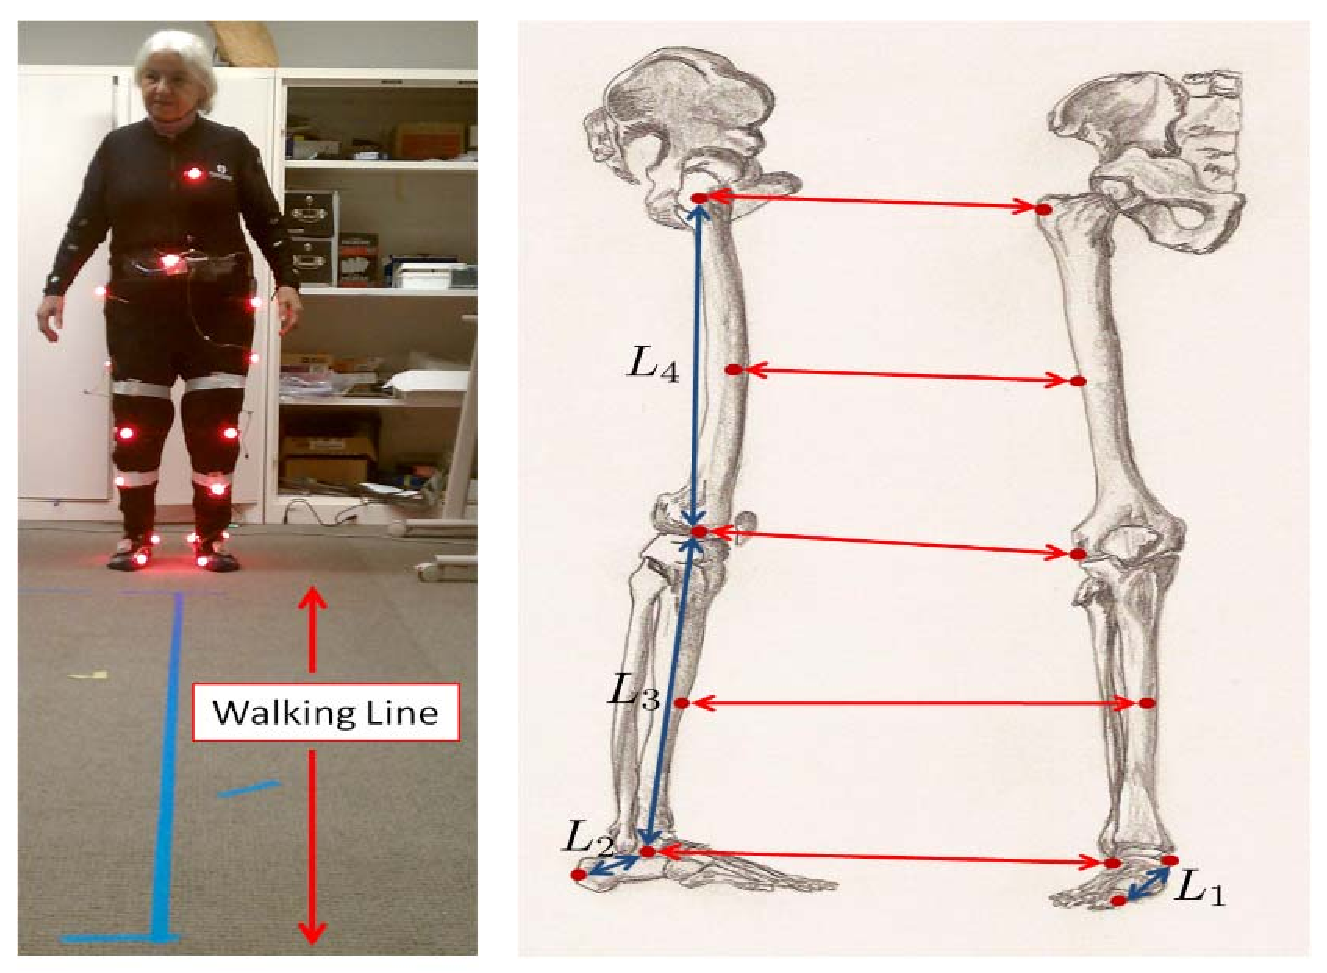
\includegraphics[width=0.7\textwidth]{LabeledDiagram}
  \caption[Illustrations of the experimental setup and sensor
  placement.]{Illustrations of the experimental setup (left) and sensor
    placement (right).
    %
    Each subject in the experiment was required to wear a suit where the LED
    sensors are fastened in place.
    %
    The sensors were placed at the joints as illustrated with the red dots on
    the right lateral and anterior aspects of the right leg.
    %
    Sensors were placed identically on the left leg.
    %
    The same sensors drawn from different views are connected with red arrows.
    %
    The blue arrows illustrate the leg segment lengths of interest,
    i.e. $L_{1}$, $L_{2}$, $L_{3}$, $L_{4}$.
    %
    The diversity of the subjects with respect to these lengths can be seen in
    \tabref{tab:measurements}.}
  \label{fig:Sensors}
\end{figure}

\begin{table}[t!]
  % \HRule
  % \vspace{2mm}

  \centering
  \caption[Measurements describing each of the subjects.]{Measurements
    describing each of the subjects.
    %
    The subject number is in the left column and the $L_1,L_2,L_3,L_4$
    measurements correspond to the lengths described in \figref{fig:Sensors}.
    %
    The anthropometric measurements in column $4$ are in kilograms and the
    measurements in columns $5$--$9$ are in centimeters.}
  \begin{tabular}{|c|c|c|c|c|c|c|c|c|}
    \hline
    & \!Sex\! & \!Age\! &  \!Weight\! & \!Height\! & $L_1$ & $L_2$ & $L_3$ &
    $L_4$ \\ \hline
    1 & M & 30 & 90.7& 184& 14.5& 8.5& 43.0& 44.0 \\ \hline
    2 & F & 19 & 53.5& 164& 15.0& 8.0& 41.0& 44.0\\ \hline
    3 & M & 17 & 83.9& 189& 16.5& 8.0& 45.5& 55.5 \\ \hline
    4 & M & 22 & 90.7& 170& 14.5& 9.0& 43.0& 39.0\\ \hline
    5 & M & 30 & 68.9& 170& 15.0& 8.0& 43.0& 43.0\\ \hline
    6 & M & 29 & 59.8& 161& 14.0& 8.5& 37.0& 40.0\\ \hline
    7 & M & 26 & 58.9& 164& 14.0& 9.0& 39.0& 41.0\\ \hline
    8 & F & 77 & 63.5& 163& 14.0& 8.0& 40.0& 42.0\\ \hline
    9 & F & 23 & 47.6& 165& 15.0& 8.0& 45.0& 43.0\\ \hline
  \end{tabular}
  \label{tab:measurements}
\end{table}


\begin{figure}[t!]
  \centering
  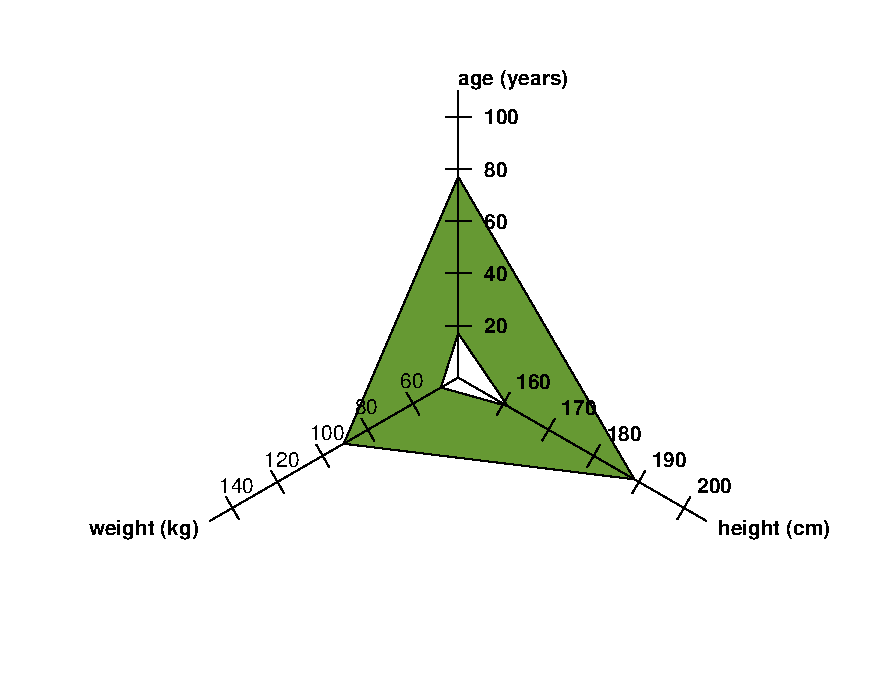
\includegraphics[width=0.7\textwidth]{subject_range_graph}
  \caption{The ranges of age, height, and mass of the test subjects.}
  \label{fig:subject-ranges}
\end{figure}

\subsection{Walking Experiment}

The data used in this work are taken from an experiment described in
\cite{Ames2011a}.
%
A summary of the collection procedure is provided for reference:
%
data were collected on nine subjects using the Phase Space System%
%
\footnote{\url{http://www.phasespace.com/}}\xspace
%
which computes the 3D position of $19$ LED sensors at $480$ frames per second
using $12$ cameras.
%
The cameras were calibrated prior to the experiment and were placed to achieve a
one millimeter level of accuracy for a space of size five by five by five meters
cubed.
%
Eight LED sensors were placed on each leg at the joints and on the heel and toe
as shown in \figref{fig:Sensors}, one LED sensor was placed on the sternum, one
LED sensor was placed on the back behind the sternum, and one LED sensor was
placed on the umbilicus.

\begin{figure}[t!]
  \centering
  \subfloat[Heel height]{
    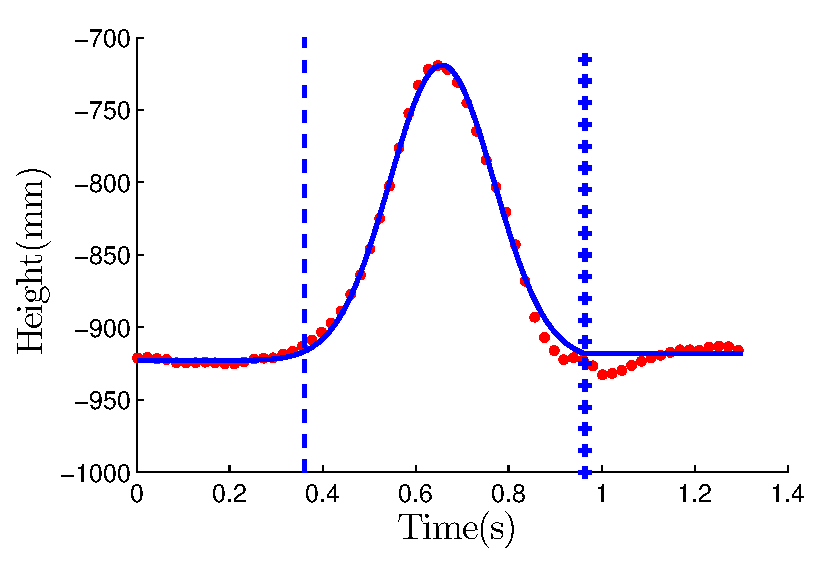
\includegraphics[width=0.48\columnwidth]{LeftHeel}
    \label{fig:heelheight}
  }
  \subfloat[Toe height]{
    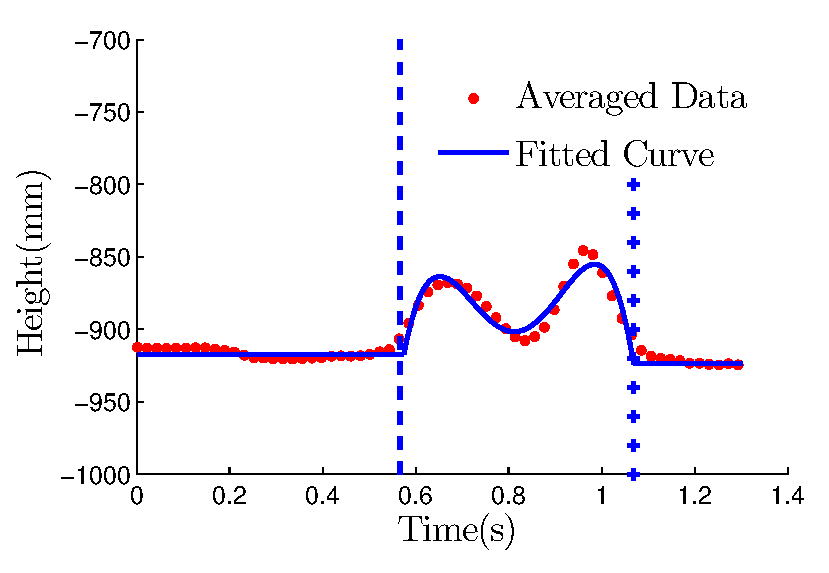
\includegraphics[width=0.48\columnwidth]{LeftToe}
    \label{fig:toeheight}
  }
  \caption[The data for the heights of the heel and toe.]{The data for the
    heights of the heel and toe.
    %
    Also shown are the fittings of a constant$\to$Gaussian$\to$constant for the
    heel and a constant$\to$fourth-order polynomial$\to$constant for the toe.
    %
    The vertical lines on the left and right indicate the lift and strike times,
    respectively.}
  \label{fig:heeltoefit}
\end{figure}

Each trial of the experiment required the subject to walk three meters along a
straight line drawn on the floor.
%
Each subject performed $12$ trials which constituted a single experiment.
%
Three female and six male subjects were tested with ages ranging between $17$
and $77$ years, heights ranging between $161$ and $189$ centimeters, and masses
ranging between $47.6$ and $90.7$ kilograms.
%
\tabref{tab:measurements} describes the measurements of each of the subjects and
a visual representation is given in \figref{fig:subject-ranges}.
%
The data for each individual were rotated so the walking occurs in the
$x$-direction and, for each subject, the $12$ walking trials were averaged
(after appropriately shifting the data in time) which resulted in a single
trajectory for each constraint for each subject for at least two steps (one step
per leg); the resulting data can be seen in \figref{fig:heeltoefit}.


\subsection{Function Fitting}

In order to determine the domain breakdowns for the subjects in the walking
experiment, it is necessary to determine the times when the human--ground
contact points change, i.e., the {\em event times}.
%
Rather than looking for when the contact point is constrained (through
thresholds), one can look for the ``simplest'' function that the contact point
follows when not enforced.
%
Then, for the domains in which the constraint {\em is not} enforced, use the
simple function; in the other domains, those in which the constraint {\em is}
enforced, fit a flat line to the constraint as it should be essentially
constant.
%
This is an optimization problem which can be stated as follows:
\begin{enumerate}
\item Select a simple function which is qualitatively similar to the trajectory
  of the constraint in the domains in which it is not enforced and choose an
  initial guess for the event times.
\item Create the fitted function as a piecewise combination of the chosen
  function fitted to the data in the domains in which the constraint {\em is
    not} enforced and a flat line fitted to the data in the domains in which
  the constraint {\em is} enforced.
\item Compute the cost function as the sum of squares of the difference between
  the data and value of the fitted trajectory at each datum for one full step
  (one step with each leg).
\item Minimize the cost function by choosing a new guess for the event times
  and then repeating steps 2--4.
\end{enumerate}

To formalize the idea of function fitting to determine event times, given a set
of contact points $\C$, let $s_{c}(t, a_{c})$ be the ``simplest'' function that
a given contact point $c \in \C$ follows when not in contact with the ground;
%
here $a_{c} \in R^{n_{c}}$ is a collection of parameters for the function
$s_{c}(t, a_{c})$ corresponding to contact point $c$.
%
Denote the indexed human data for contact point $c$ by $y_{c}[k]$, with
$\tau[k]$ the time corresponding to datum $y_{c}[k]$ for discrete index variable
$k \in \{1,\ldots,T\}$.
%
When the contact point is constrained, it is constant, and when it is
unconstrained, it follows $s_{c}(t, a_{c})$.
%
For each contact point $c \in \C$, consider the function:
%
\begin{align*}
  f_{c}(t, k_{c}^{\ell}, k_{c}^{s}, a_{c}) =  \left\{\begin{array}{l l}
      s_{c}(\tau[k_{c}^{\ell}], a_{c}), & \hspace{2mm} t \leq
      \tau[k_{c}^{\ell}],\\
      s_{c}(t, a_{c}), & \hspace{2mm} \tau[k_{c}^{\ell}] < t <
      \tau[k_{c}^{s}],\\
      s_{c}(\tau[k_{c}^{s}], a_{c}), & \hspace{2mm} \tau[k_{c}^{s}] \leq t,\\
  \end{array} \right.
\end{align*}
where $\tau[k_{c}^{\ell}], \tau[k_{c}^{s}] \in \{\tau[k]\}_{k = 1}^{T}$ are the
event times indicating when contact point $c$ becomes unconstrained (lift) and
constrained (strike), respectively.
%
It is assumed that $k_{c}^{\ell} < k_{c}^{s}$.
%
If this is not the case, then $f_{c}$ would consist of the ``simplest''
function, followed by a constant, followed by the ``simplest'' function.
%
After the construction of the $f_{c}$ functions in this chapter, the optimization
parameters are supressed---i.e., $f_{c}(t) = f_{c}(t, k_{c}^{\ell}, k_{c}^{s},
a_{c})$---but it is assumed they have been determined.
%
To calculate the event times as they best fit the data, one must solve the
following optimization problem
\begin{align*}
  \min_{k_{c}^{\ell}, k_{c}^{s} \in \{1, \ldots, T\}} \ \min_{a_{c} \in
    \R^{n_{c}}} \ \sum_{k = 1}^{T} \left( f_{c}(t, k_{c}^{\ell}, k_{c}^{s},
    a_{c}) - y_{c}(t) \right)^2
\end{align*}
for each $c \in \C$.
%
In the case of humans with flat feet, there are four constraints of interest:
%
one at the heel and one at the toe for both the left and right feet.
%
Since each constraint has a lift and strike time, there is a total of eight
domains in one whole step.
%
However, when referring to a step in robotics, researchers typically use stance
and non-stance legs;
%
without the distinction of left and right, the system is reduced to a
four-domain model.
%
Doing this allows one to exploit the symmetry inherent in bipedal walking to
simplfy controller design.

To illustrate this procedure, consider the averaged data for the heel and toe
shown in \figref{fig:heeltoefit}.
%
Looking at these data, the trajectory of the heel appears to follow a constant,
followed by a Gaussian, followed by a constant.
%
In a similar fashion, the averaged data for the toe appear to follow a constant,
followed by a fourth-order polynomial, followed by a constant.
%
With these observations in hand, fit the averaged heel and toe data to these
functions using the described procedure.
%
The results of the fitting procedure are shown in the topmost graph of
\figref{fig:heeltoefit};
%
the transition points $\tau[k_{c}^{\ell}]$ and $\tau[k_{c}^{s}]$ are indicated
by vertical lines.
%
The fits quite accurately represent the data given the simplicity of the
functions chosen;
%
to quantify this, the coefficients of correlatation are $0.9968$ for the heel
and $0.9699$ for the toe.


\subsection{Determining the Domain Breakdown}

Given the data for a contact point $c \in \C$, the lift and strike times are
determined for each contact point, $\tau[k_{c}^{\ell}]$ and $\tau[k_{c}^{s}]$
for $c \in \C =  \{c_{1},c_{2},c_{3},c_{4}\} = \{\clh, \clt, \crh, \crt\}$, over
the time interval of the averaged data, $\big[\tau[1], \tau[T]\big]$, using the
aforementioned techniques.
%
Since the data comprise at least two steps (one step with each leg), there are
multiple lift and strike times over the period of the data.
%
Denote by $\mathcal{J}_{c} \subset \big[\tau[1], \tau[T]\big]$ the period where
the constraints associated with a contact point are enforced, i.e., $t \in
\mathcal{J}_{c}$ if $f_{c}(t) = \mathrm{constant}$ with $f_{c}$ the fitting
function for the contact point $c \in \C$; these intervals are shown in blue in
\figref{fig:domainbreakdown} over the course of one step (not the entire data
period) in the case of $\C =  \{\clh, \clt, \crh, \crt\}$.
%
Analogous to the definition of a domain breakdown
(\defref{def:domainbreakdown}), one can define a binary vector, $b(t) \in
\Z_{2}^{|\C|}$ with $|\C|$ representing the cardinality of $\C$, encoding which
contact points are constrained at any given time by letting $b_{i}(t) = 1$ if $t
\in \mathcal{J}_{c_{i}}$ for $i \in \{1, \ldots, |\C|\}$.

To determine the domain breakdown associated with walking, begin by defining the
directed cycle $\Gamma$ (if it exists, which is not guaranteed).
%
The function $b(t)$ takes on only a finite number of values, say, $N$ values;
%
let these values be represented by $d[n]$ for $i \in \{1, \ldots, N\}$.
%
For the walking to be periodic, there must exist a positive value of $p \in \Z$
satisfying
\begin{align}
  \label{eq:dstep}
  d[n + p] =
  \left[\begin{array}{c c}
      \boldzero & I\\
      I & \boldzero
    \end{array}\right] d[n]
\end{align}
for $n \in \{1, \ldots, N-p\}$ with $I$ the identity matrix and $\boldzero, I
\in \R^{\frac{|\C|}{2} \times \frac{|\C|}{2}}$.
%
\begin{figure}[t!]
  \centering
  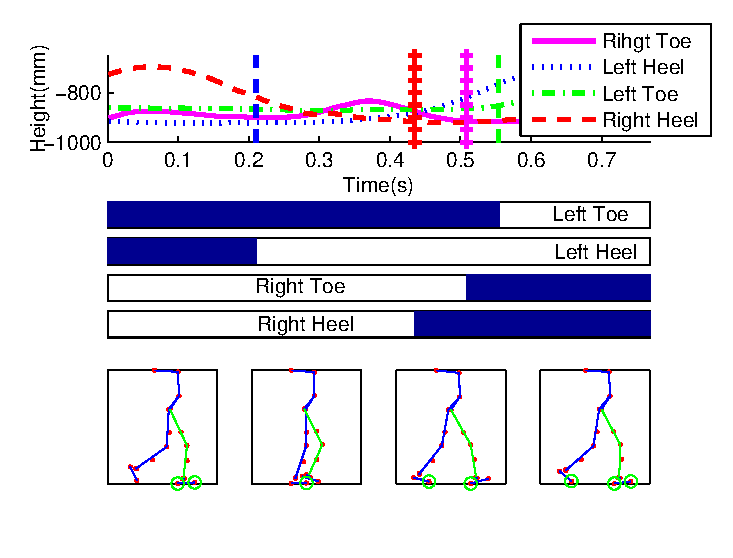
\includegraphics[width=0.8\columnwidth]{domainbreaking}
  \caption[An overview of how the domain breakdown is achieved.]{An overview of
    how the domain breakdown is achieved.
    %
    The top row illustrates the height of the toe and heel of each leg over one
    step along with the lifting and strike time for each constraint (illustrated
    with vertical lines).
    %
    The middle row illustrates which constraints are active based upon the
    fitting.
    %
    The bottom row is the resulting domain breakdown where enforced constraints
    are drawn in green circles.}
  \label{fig:domainbreakdown}
\end{figure}
%
Note: if the data constitute multiple steps, there will be more than one
possible value for $p$;
%
in this case, the proper value of $p$ is the smallest of these values as this
represents one step.
%
The matrix that is premultiplied by $d[n]$ serves the purpose of reordering the
right leg and left leg.
%
If this $p$ can be found, periodic walking over the course of two steps has been
discovered in the data with the behavior of the left leg mirroring the behavior
of the right leg.
%
In this case, one constructs a directed cycle with $p$ domains (as in
\eqref{eq:directedcyclep}) and this is the graph $\Gamma$.
%
The corresponding domain breakdown $\B$ is given by $\B(v_{n}) = d[n]$ for $n
\in \{1, \ldots, p\}$.
%
The application of this procedure to a single subject can be seen in
\figref{fig:domainbreakdown}.


\subsection{Results}

The outlined process is performed on the set of contact points $\C =  \{\clh,
\clt, \crh , \crt\}$ for the nine test subjects that performed the walking
experiment.
%
The end result showed that each subject had the same, {\em universal}, domain
breakdown; this can be seen in \figref{fig:domaingraph}.
%
In the context of this work, a single subject was chosen for study based upon
the completeness of the sensor data, which, in this case, was subject four; the
domain breakdown and the time spent in each domain for the subject can be seen
in \figref{fred}.
%
It is important to note that the results are consistent with those found in the biomechanics
literature.
%
Specifically, performing the breakdown process on data from the literature
\cite{Winter2009} resulted in the same domain breakdown.
%
Additionally, the amount of time spent having single and double support are
similar to previous studies \cite{Ackermann2007}.

\begin{figure}[t]
  \centering
  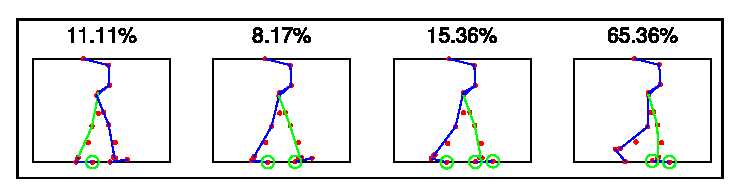
\includegraphics[width=1.0\columnwidth]{test_subject_4}
  \caption{The domain breakdown for subject four together with the amount of
    time spent in each domain.
    %
    Each illustration is a snapshot of the subject's configuration at the
    beginning of the domain together with the contact points enforced.}
  \label{fred}
\end{figure}


\section{Human-Inspired Controller Design}

The goal of this section is to find functions that are ``canonical'' to human
walking, i.e., outputs on the configuration of the human, such as the angle of
the knee, that seem to be intrinsic to walking.
%
These functions will be used in the design of control laws, for a bipedal robot
with anthropomorphic measurements, using the standard method of input/output
linearization \cite{Sastry1999}.
%
This control design strategy results in anthropomorphic walking behavior.


\subsection{``Canonical'' Walking Functions} \label{sec:functions}

Rather than just using trajectories from the human data, functions are sought
which have both ``simple'' representations (much like in the case of heel and
toe height discussed in \secref{sec:domainbreakdown}) and appear to be intrinsic
to human walking.
%
From the perspective of control, these functions must not conflict with the
constraints of the system on each domain resulting from the enforced contact
points as dictated by the domain breakdown.
%
That is, the system must not be overconstrained.

Data is considered from subject four; these data are obtained through the
process outlined in \secref{sec:domainbreakdown}.
%
(Subject four's data were selected as they contain the least noise.)
%
A variety of functions are inspected---these represent different fundamental
behaviors of human walking, e.g., the movement of the torso or of the legs.
%
Examination of the human data, reveals that functions describing the behavior of
the torso, the hip, the non-stance leg slope (the slope of the line connecting
the non-stance ankle to the hip), the knee angles, and the heel and toe heights
seem to encode the most fundamental behaviors related to walking, as dictated by
the correlation between the data and the fitted functions.
%
The human behavior of these different functions throughout the course of the
walking gait can be seen in \figref{fig:constraints-fitting}, with the data
beginning at the start of domain $ts$.

\begin{figure}[ht!]
  \centering
  \subfloat[Angular constraints]{
    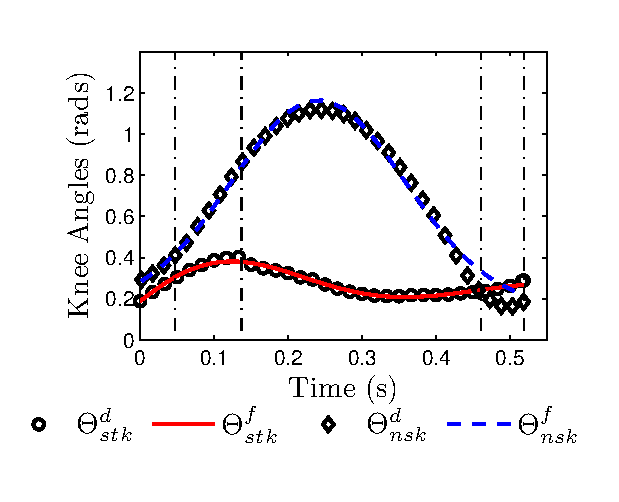
\includegraphics[width=0.48\textwidth]{constraints_angles}
    \label{fig:constraints-knees}
  }
  \subfloat[Slope constraints]{
   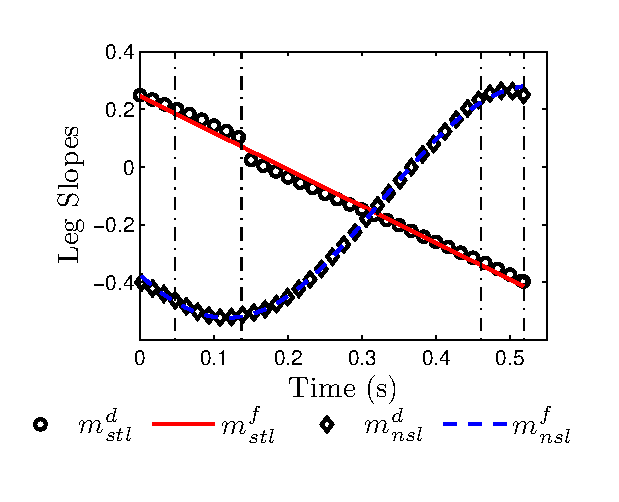
\includegraphics[width=0.48\textwidth]{constraints_slopes}
    \label{fig:constraints-legs}
  }\\
  \subfloat[Height constraints]{
    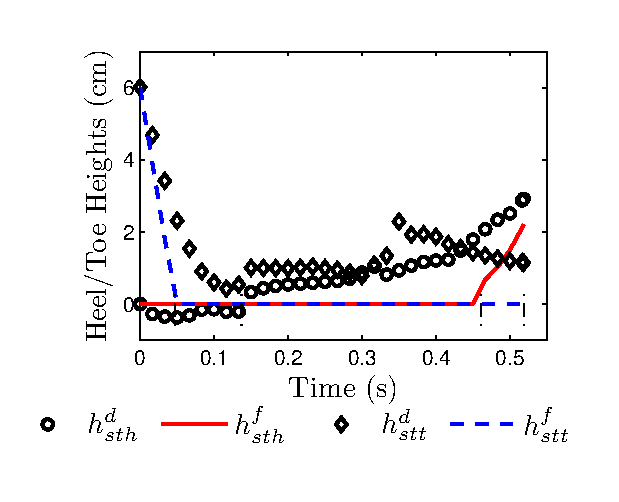
\includegraphics[width=0.48\textwidth]{constraints_heights}
    \label{fig:constraints-heights}
  }
  \caption{Human data over the course of one step with one leg and the
    ``canonical'' functions that are fitted to these data.
    %
    $d$ superscripts represent the data and $f$ superscripts represent the fits.
    %
    The plots start at the beginning of the domain {\DA}, with vertical lines
    indicating when transitions between domains occur.
    %
    The specific variables that are plotted can be seen in
    \figref{fig:robotconstraints}.}
  \label{fig:constraints-fitting}
\end{figure}

Before further detail is given, a remark on the choice of constraints is in
order:
%
\begin{remark} \label{rmk:actuation}
  When choosing which functions to track, it is important to consider which
  joints will have actuation and which actuators will do most of the work
  necessary to track a given constraint.
  %
  An example of a poor choice of constraints would be the stance knee, the
  stance leg slope, and the stance hip position.
  %
  The reason this is a poor choice is as follows:
  %
  to track these three constraints, only two degrees of actuation will do most
  of the work---the stance ankle and the stance knee.
  %
  Thus, the dynamics of the system will be ill-behaved.
  %
  Indeed, if one tries to track three constraints on a two-link pendulum, the
  result will be an overconstrained system {\em unless} two of the constraints
  match up perfectly---in other words, two {\em independent} constraints are
  being tracked.
  %
  This same argument extends to the specified robot, which is a multi-link
  kinematic chain.
  %
  Examples of reasonable output choices can be found in \cite{Sinnet2014}.
\end{remark}


\subsubsection{Knee}

Inspecting the behavior of the human knee over the course of the gait (see
\figref{fig:constraints-knees}) reveals that the angle of the human knee appears
to follow a Gaussian when it is swinging (the non-stance leg) and a second order
system response (i.e., the step response of a spring damper system) when the
weight of the person is on the leg (i.e., when the leg is the stance leg).
%
With this in mind, the following functions are fit to the human data for the
knee angles of the stance and non-stance legs:
%
\begin{align*}
  y_{d,\cnsk}(t) &= A_{5,1} \, \exp\left(\frac{-(t-A_{5,2})^2}{2
      (A_{5,3})^2}\right) + A_{5,4},\\
  y_{d,\cstk}(t) &= -A_{2,1} \, \frac{\cos(A_{2,2}\,t)-A_{2,3}
    \sin(A_{2,2}\,t)}{\exp(A_{2,4} \, t)} + A_{2,5}. 
\end{align*}
%

An intuitive explanation of this is as follows:
%
when the leg is in ``stance'' mode, the human knee acts like a spring-damper
system responding to the impulse of the human as he or she puts his or her body
weight on the stance leg---that is, the human tries to prevent the leg from
collapsing by stiffening it, resulting in a spring-damper effect.
%
When the human leg is in ``non-stance'' mode, the weight of the human is
primarily not on it, so the knee is free to swing---there is no reason to keep
the leg stiff.


\subsubsection{Leg}

In the data for the slope of the non-stance leg as seen in
\figref{fig:constraints-legs}---here, leg is defined as the straight line
connecting the ankle to the hip---the slope appears to follow a sinusoid; thus
the following function is fit:
%
\begin{align*}
  y_{d,nslm}(t) &= A_{6,1} \, \sin(A_{6,2} \, t + A_{6,3}) + A_{6,4}.
\end{align*}
%
Intuitively, this just means that the non-stance leg swings freely much like the
non-stance knee.
%
Note that while it is possible to choose the slope of the stance leg as a
constraint to track---indeed, a simple function can be fitted to the slope of
the stance leg---the forward velocity of the hip is instead chosen.
%
In terms of time-control this will not make much of a difference, but the reader
will see that, when the control is migrated to pure feedback, tracking the hip
velocity will allow for direct control over walking speed.


\subsubsection{Hip}

The behavior of the hip is quite simple.
%
Examination of the data reveals that the hip moves forward monotically in time
at an approximately constant rate.
%
However, instead of tracking the position of the hip, the velocity of the hip is
instead tracked, thus motivating the following function:
%
\begin{align*}
  y_{d,hv} = A_{3,1}.
\end{align*}
%
The reason for tracking the velocity instead of the position is related to the
method used to impose feedback control on the system and requires some
explanation; however, due to the level of detail, this discussion will be
deferred until later.
%
It is of interest, however, to note that, as mentioned previously, tracking hip
velocity allows for direct control over the walking speed of the robot.


\subsubsection{Torso}

The data show that a human tends to keep his or her torso upright throughout his
or her walking gait.
%
Specifically, the data indicates that the absolute angle of the torso with
respect to the world frame closely follows a sine wave, but the amplitude is
small, so it is approximated with a constant:
%
\begin{align*}
  y_{d,T\angle} &= A_{4,1}.
\end{align*}
%
Note that, the choice of tracking a constant results in a poor correlation
between the function and data; however, one can argue that the tiny amount of
motion from the torso has very little effect on the overall gait.


\subsubsection{Ankle}

When the non-stance leg is swinging, to prevent the non-stance ankle from
rotating freely, the behavior of the ankle angle is approximated by a constant:
%
\begin{align*}
  y_{d,nsa\angle} &= A_{8,1}.
\end{align*}
%
One can justify this choice by claiming that the motion of the ankle has only a
marginal effect on the overall gait provided that ground clearance is not an
issue.
%
As in the case of the torso, the correlation between this fit and the data will
not be good but, again, this does not have a large effect on the gait.


\subsubsection{Foot}

Finally, the behaviors of the heel and toe are found to be significantly more
complicated than the previously discussed behaviors, as can be seen in
\figref{fig:constraints-heights}.
%
Although the actual functions describing these heights are quite simple (see
\figref{fig:heeltoefit}), it is generally not effective to follow these
functions---see \rmkref{rmk:dimconst}.
%
Since the foot is constrained during certain phases of the gait, it would not
make sense to track the constrained points during these phases.
%
Therefore, the behavior of the feet is segmented based on the domain breakdown
of the human gait.
%
In particular, the transition from domain {\DA} to domain {\DB} occurs when the
stance toe strikes the ground, and, in fact, it is found that the height of the
toe approximately follows a constant as it approaches the ground in domain
{\DA}.
%
In order to satisfy this local objective, an attempt is made to track the height
of the toe using the following function:
%
\begin{align*}
  y_{d,\cstth}(t) = A_{7,1} \, t + A_{7,2}.
\end{align*}
%
After domain {\DA}, the toe is fixed to the ground and thus, is no longer
tracked.
%
In a similar light, when domain {\DC} is reached, the goal is to effect heel
lift.
%
As such, analysis of the data reveals that non-stance heel begins to lift
approximately according to a Gaussian, thus motivating the following function:
%
\begin{align*}
  y_{d,\csthh}(t) &= A_{1,1} \, \exp\left(\frac{-(t-A_{1,2})^2}{2 (A_{1,3})^2}\right) + A_{1,4}.
\end{align*}

\begin{remark} \label{rmk:dimconst}
  Certain constraint functions represent dimensionalized constraints, e.g., heel
  height, whereas other functions discussed, e.g., angles and slopes, represent
  nondimensionalized constraints.
  %
  In general it is not effective to follow dimensionalized constraints as they
  represent constraints on specific points of the system and thus have the
  potential to introduce extreme restrictions on the configuration space of the
  entire system.
  %
  This should be thought of in terms of the inverse kinematics problem:
  %
  consider an end-effector and solve for the range of possible configurations on
  the angles leading up to that point.
  %
  Thus, dimensionalized constraints are not robust with respect to length
  parameters.
  %
  Additionally, these dimensionalized constraints can conflict with other
  holonomic constraints being tracked.
  %
  Recall that the intent is to track the height of the stance toe;
  %
  in this case, the issue of configuration restriction is minimal:
  %
  only the heel is pinned to the ground so tracking the toe's height is
  equivalent to tracking the angle or slope of the foot.
\end{remark}

\begin{figure}[t!]
  \centering
  \subfloat[Robot configuration]{
    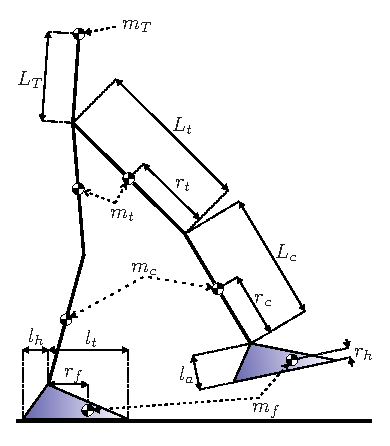
\includegraphics[width=.4\columnwidth]{robot_config}
    \label{fig:roboconf}
  }
  \hspace{.2cm}
  \subfloat[Tracking outputs]{
    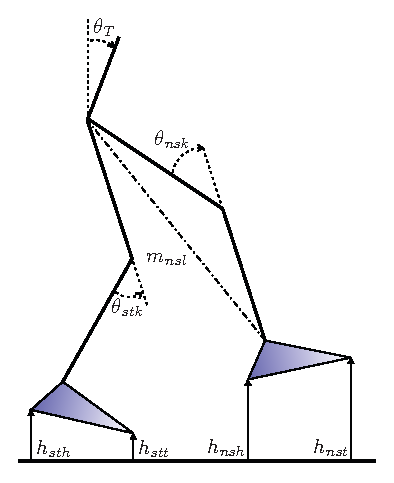
\includegraphics[width=.4\columnwidth]{robot_const}
    \label{fig:trackingoutputs}
  }
  \caption[Kinematic and dynamic model of the 2D bipedal robot.]{Kinematic and
    dynamic model of the 2D bipedal robot:
    % 
    (a) The general configuration of the 2D bipedal robot with knees and feet;
    % 
    (b) The different configuration-based outputs considered in the fitting of
    the ``canonical'' functions.}
  \label{fig:robotconstraints}
\end{figure}


\subsubsection{Fitting}

The paramaters of the ``canonical'' functions can be found by minimizing the
error between the human data and the corresponding functions.
%
Formally, given a function choice $y_d(t, A)$, with $A \in \R^{n_{d}}$ the $n_d$
parameters, and the corresponding data function $x_{d}[k]$ with indexed time
$\tau_{d}[k]$ for data index $k \in \{1, \ldots, K\}$ (for $K$ data points), a
solution is sought for the optimization problem:
%
\begin{align}
  \label{eq:fitsolve}
  \min_{A \in \R^{n_{d}}} \sum_{k=1}^{K} (y_{d}(\tau_{d}[k], A) - x_{d}[k])^2.
\end{align}
%
The fits that result from solving \eqref{eq:fitsolve} are shown in
\figref{fig:constraints-fitting}.
%
The correlation coefficient for the fits of each of the respective functions can
be found in \tabref{tab:fitcor}.
%
In all cases (with the exception of the torso and ankle), the fits are very
good.
%
One final note of import:
%
in order to achieve walking in simulation, some parameters had to be tweaked by
hand;
%
the parameters generated as well as the tweaked parameters can be found in
\tabref{tab:funcparam}.

\begin{table*}[t!]
  %\HRule
  \centering
  \caption[Correlations of fitted functions and usage on each
  domain.]{Correlations of fitted functions and usage on each domain.
    %
    Note that many fits have extremely high correlations.
    %
    For the four right columns, a $\bullet$ indicates the constraint for that
    row is tracked on the corresponding domain.
  }
  \begin{tabular}{| c | l | c || c | c | c | c |}
    \hline
        {\bf Eq.} & {\bf Constraint} & $r$ & $\DA$ & $\DB$ & $\DC$ & $\DD$\\
        \hline
        $y_{d,sthh}$ & Stance heel height & 0.73671 & & & & $\bullet$ \\
        \hline
        $y_{d,stk\angle}$ & Stance knee angle & 0.99213 & $\bullet$ & $\bullet$
        & $\bullet$ & $\bullet$ \\
        \hline
        $y_{d,hv}$ & Hip forward velocity  & * & $\bullet$ & $\bullet$ &
        $\bullet$ & $\bullet$ \\
        \hline
        $y_{d,T\angle}$ & Torso absolute angle & * & $\bullet$ & $\bullet$ &
        $\bullet$ & $\bullet$ \\
        \hline
        $y_{d,nsk\angle}$ & Non-stance knee angle & 0.99301 & $\bullet$ &
        $\bullet$ & $\bullet$ & $\bullet$ \\
        \hline
        $y_{d,nslm}$ & Non-stance leg slope & 0.99971 & & & $\bullet$ & \\
        \hline
        $y_{d,stth}$ & Stance toe height & 0.99971 & $\bullet$ & & &\\
        \hline
        $y_{d,nsa\angle}$ & Non-stance ankle angle & * & & & $\bullet$ &
        $\bullet$\\
        \hline
  \end{tabular}
  \label{tab:fitcor}
\end{table*}

\begin{table}[t!]
  % \HRule
  \caption[Human function parameters.]{Human function parameters.
    %
    Asterisks (*) denote no additional parameters.}
  \centering
  \begin{align*}
    A = \left[\begin{array}{c c c c c}
        % sthh
        0.2039 & 0.7540 & 0.1109 & 0.0000 & *\\
        % stka
        0.0710 & 13.3920 & 2.6671 & 3.7440 & 0.1881\\
        % hv
        1.1771 & * & * & * & *\\
        % Ta
        0.0595 & * & * & * & *\\
        % nska
        1.1500 & 0.2480 & 0.1170 &0.1669 & *\\
        % nslm
        0.4035 & 7.5204 & -2.4442 & -0.1202 & *\\
        % stth
        -0.1638 & 0.0078 & * & * & *\\
        % nsaa
        -0.0800 & * & * & * & *        
      \end{array}\right]
  \end{align*}
  \label{tab:funcparam}
\end{table}



\subsection{Robotic Hybrid Model \& Controllers}

Consider the robotic walker shown in \figref{fig:robotconstraints}.
%
The goal is to use the human-inspired domain breakdown and ``canonical'' walking
functions to design controllers for this robot.


\subsubsection{Robotic Model}

It was shown in \secref{sec:complex-models} that, given a collection of contact
points and a domain breakdown (defined on a cycle graph), one can explicitly
construct a hybrid control system.
%
In particular, using the procedure discussed, a domain breakdown $\B$ is
obtained, which is associated to human walking (see
\exmpref{ex:domainbreakdown}) defined on the cycle $\Gamma_u = (V, \, E)$ (given
in \exmpref{universalgraph}).
%
As a result of the construction in \secref{sec:complex-models}, one obtains a
hybrid control system describing this robot:
%
\begin{align}
  \label{eq:hcstime}
  \HCS = (\Gamma, \D, \U, \Guard, \Delta, \FG).
\end{align}
%
\begin{figure}[t!]
  \centering
  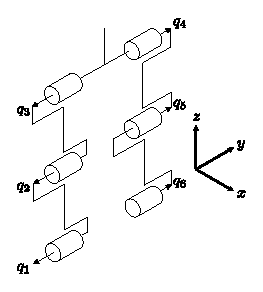
\includegraphics[width=.45\columnwidth]{robot_angles}
  \caption[The shape coordinates for the biped labeled $q_i$.]{The shape
    coordinates for the biped labeled $q_i$.
    %
    The corresponding arrows represent twists. The $x$-axis is coming out of the
    page.
    %
    The hip width is zero and is shown for illustration purposes only.
    %
    The axes shown represents the body-fixed frame which has orientation about
    the $y$-axis given by $\phi_b$.}
  \label{fig:shapecoords}
\end{figure}
%
As discussed previously, attach a reference frame $\Rb$ to the hip. Let $\phi_b$
be the orientation of $\Rb$ (with respect to the $y$-axis for a two-dimensional
model) and let $p_b^x, p_b^z$ be the Cartesian position of $\Rb$.
%
The shape coordinates $\qs$ for the biped are chosen to be the relative angles
between any two successive links starting at the stance foot as shown in
\figref{fig:shapecoords}.
%
Combining $\phi_b$, $p_b^x$, $p_b^z$, and $\qs$ gives the configuration space
for the biped.
%
The only unknowns for the model are the physical parameters of the system;
%
these are obtained from the anthropometric data for subject four, given in
\tabref{tab:measurements}.
%
In particular, the lengths are given and the mass of each point mass in the
robot (as seen in \figref{fig:robotconstraints}) is estimated from the overall
mass of the person using a standard mass distribution of a human from the
literature \cite{Winter2009}.


\subsubsection{Controller Design}

The goal now is to design a controller to track the desired functions given in
\secref{sec:functions}.
%
Before discussing which of these functions are tracked on each domain, a
description technique used to track the desired functions, input/output
linearization \cite[Ch.~9]{Sastry1999}, is given. % Sastry, pp. 407

Consider a control system of the form $(\xfv, \, \xgv)$, $\vinV$ as given in
\defref{def:hcs} for an arbitrary domain in the domain breakdown.
%
Let $y^{a}_{v}\argsq$ represent the vector of ``actual'' outputs on the system
(e.g., the height of the stance heel)---these can be found by computation of
forward kinematics \cite{Murray1994}.
%
Let $y^{d}_{v}\argt$ represent the vector of ``desired'' output functions to be
tracked, which consists of combinations of the human-based ``canonical''
constraint functions.
%
Let $n = \dim(Q)$ and let $m$ be the number of constraint functions being
tracked on a given domain.
%
Motivated by the desire to drive $y^{a}_{v}(\q\argt) \to y^{d}_{v}\argt$ as $t
\to \infty$, a definition is given for the following virtual output vector:
%
\begin{align}
  \label{eq:virtout}
  y_v(\q, t) = y^a_v\argsq - y^d_v\argt.
\end{align}
As the functions tracked consists of both positions and velocities, the system
has mixed relative degree.
%
That is, the output corresponding to velocity will have relative degree one
whereas the outputs corresponding to positions will each have relative degree
two.
%
Reorder the outputs as follows:
\begin{align}
  \label{eq:vouts}
  y_v(\q, \dq, t) = (y_{v,1}(\q, \dq, t), y_{v,2}(\q, t))
\end{align}
with $y_{v,1}$ a vector containing the relative-degree-one outputs and $y_{v,2}$
a vector containing the relative-degree-two outputs.
%
(In this thesis, $y_{v,1}$ is a scalar.)
%
A control law which drives \eqref{eq:vouts} to zero is
\begin{align*}
  \lefteqn{u(\q, \dq, t) = }\\
  &&-\mathcal{A}_{v}^{-1}(\q, \dq, t)
  \left(\left[\!\!\begin{array}{c}
      0\\
      L_{\xfv} L_{\xfv} y_{v,2}(\q, t)
    \end{array}\!\!\right]
  + \left[\!\!\begin{array}{c}
      L_{\xfv} y_{v,1}(\q, \dq, t)\\
      2 \varepsilon L_{\xfv} y_{v,2}(\q, t)
    \end{array}\!\!\right] +
  \left[\!\!\begin{array}{c}
      \varepsilon y_{v,1}(\q, \dq, t)\\
      \varepsilon^2 y_{v,2}(\q, t)
    \end{array}\!\!\right]\right),
\end{align*}
with $\mathcal{A}_{v}(\q, \dq, t)$ the decoupling matrix given by
\begin{align*}
  \mathcal{A}_{v}(\q, \dq, t) =
  \left[\begin{array}{c}
      L_{\xgv} y_{v,1} (\q, \dq, t)\\
      L_{\xgv} L_{\xfv} y_{v,2}(\q, t)
    \end{array}\right],
\end{align*}
where, again, $(\xfv, \, \xgv)$ is given in \defref{def:hcs}.
%
In the above,
\begin{align*}
  L_{\xfv} y(\q, \dq, t) = \pd{y(\q, \dq, t)}{(\q, \dq, t)} \cdot
  \xfv(\q, \dq, t)
\end{align*}
represents the Lie derivative with $\q, \dq, t$ representing independent
variables.
%the control field $g_v(q)$ is given by
%\begin{align}
%    g_v(q) = \left[\begin{array}{c}
%        \mathbf{0}_{n \times m}\\
%        D^{-1}(q) B(q)
%    \end{array}\right]
%\end{align}
%with $B(q)$ a torque distribution matrix specific to each domain. These are
%omitted but can be found online at \cite{SUP_online}.
Applying the given control law yields the non-autonomous closed-loop dynamical
system
\begin{align}
  \label{eq:clsys}
  \xf_\mathit{cl,v}(\q, \dq, t) = \xfv(\q, \dq) + \xgv\argsq \, \uu(\q, \dq, t).
\end{align}
%The corresponding hybrid system is then
%\begin{align}
%    \HS = (\D, S, R, F)
%\end{align}

Completion of the controller construction requires the specification of the
vectors $y^{a}_{v}$ and $y^{d}_{v}$ for $\vinV$ which are specific to each
of the four domains in \figref{fig:domaingraph}.
%
As mentioned previously, the vector $y^a_v$ consists of the robotic constraints
pictured in \figref{fig:robotconstraints}, which are computed directly from the
kinematics of the robot.
%
Therefore, the only decision remaining is which of the ``canonical'' human
functions to track on each domain.
%
The specific choice of functions is shown in \tabref{tab:fitcor} where black
dots indicate which functions are tracked on which domains.
%
The choice of functions is based on the discussion in \secref{sec:functions}
coupled with choosing collections of functions that do not conflict with the
holonomic constraints imposed on the system as a result of ground contact (see
Remarks \ref{rmk:actuation} and \ref{rmk:dimconst}).
%
Applying these collections of controllers to the hybrid control system
\eqref{eq:hcstime} yields the non-autonomous hybrid system:
%
\begin{align}
  \label{eq:hstime}
  \HS_{t} = (\Gamma, \, \D, \, \Guard, \, \Delta, \, \F).
\end{align}

\begin{remark}
  One final point worthy of mention is transitioning from domains with no
  impact, i.e., contact point becomes unconstrained.
  %
  Looking at equations, \eqref{eq:controlsystem} and \eqref{eq:wrench}, it is
  apparent that one can achieve lift by simply solving for a value of $\uu$
  which will cause the heel to lift.
  %
  Such a value would be outside the domain as defined in \eqref{eq:domain};
  %
  specifically, this value of $\uu$ will violate \eqref{eq:constnu}.
  %
  Provided that \eqref{eq:constnu} is satisfied during the a given phase, it
  becomes a control decision when to lift the heel or toe.
  %
  A criterion is chosen and then appropriate control is applied to
  instantaneously achieve heel or toe lift.
  %
  In the domain that follows, the control laws implicit in \eqref{eq:clsys} will
  be responsible for causing the toe or heel to continue to lift.
\end{remark}


\subsection{Simulation of Time-Based Feedback Controller} \label{sec:timesim}

This subsection presents the results of a simulation of the bipedal robot
modeled by \eqref{eq:hstime}.
%
The parameters used for the human functions are given in \tabref{tab:funcparam}.
%
It is important to note that, in order to achieve walking, it was necessary to
tweak the parameters;
%
specifically, this amounted to the multiplication of the row corresponding to
the non-stance leg slope (row six) by $1.25$.
%
Videos of the walking can be found online.%
%
\footnote{\url{http://www.rwsinnet.com/phdthesis/}\label{fn:rwsinnet}}\xspace
%
It is found through simulation that the biped has stable walking.
%
This is checked by finding a fixed point on the orbit and verifying its
stability using the \Poincare{} map technique \cite{Parker1989}.
%
Using the model parameters found online\fnref{fn:rwsinnet} and the
input/output linearization control gain $\varepsilon = 15$, the system is
simulated and the following fixed point is found:
%
\begin{align}
  q_{s,t}^{*} =
  \left(\!\!\!\!\begin{array}{c c c c c c}
    -.460 & \hphantom{-}.246 & \hphantom{-}.272 & -.441 & \hphantom{-0}.323 &
    \hphantom{-}.162
  \end{array}\!\!\right)\\
  {\dot q}_{s,t}^{*} =
  \left(\!\!\!\!\begin{array}{c c c c c c}
    -.951 & \hphantom{-}.452 & \hphantom{-}.518 & -.309 & -2.660 & -.509
  \end{array}\!\!\right)
\end{align}
which is on the guard of domain $\DC$.
%
This verifies that there exists a walking gait.
%
Note that only the shape coordinates are given for the fixed point as the other
coordinates will be completely determined by the condition that the biped is on
the guard;
%
that is, the constraints that exist on the system, e.g., the stance toe is on
the ground, are enough to uniquely determine the rest of the variables,
$\phi_b$, $p_x$, and $p_z$.

In the context of bipedal walking, a stable limit cycle or an exponentially
stable periodic orbit implies stable walking.
%
It is, therefore, desirable to show that the system has a stable limit cycle.
%
This is achieved by examining the Jacobian of the \Poincare{} map linearized
about the fixed point $(\qst, \dqst)$ \cite{Parker1989}.
%
This \Poincare{} map will be stable if all the eigenvalues of the Jacobian have
magnitude below unity.
%
Then, stability of the \Poincare{} map implies stability of the system.
%
The Jacobian matrix can be approximated by perturbing along the guard about the
fixed point with respect to the coordinates $\q$ and $\dq$.
%
A numerical approximation yields eigenvalues of the following magnitudes:
%
\begin{align}
  \label{eq:time-eigs}
  |\lambda_{t}| \in \{0.2640, \, 0.2492, \, 0.0337, \, 0.0337, \, 0.0011, \,
  \ldots\},
\end{align}
where, for the sake of space, only the five eigenvalues with the largest
magnitudes are included.
%
At this point in the discussion, a remark about zero eigenvalues is appropriate:

\begin{remark}
  When considering a \Poincare{} section $\Guard$ which is a guard of a hybrid
  system with constraints, some of the eigenvalues will be zero.
  %
  This is a result of the difference in the dimension of the Jacobian and the
  dimension of the guard which is a transverse hyperplane of the continuous
  trajectory.
  %
  Specifically, consider the guard used here as $\Guard$.
  %
  In this  case, the guard restricts the previously nine-dimensional position
  space such that the state of the system, throwing out cyclic variables such as
  $x$-position, can be determined completely using only six position variables.
  %
  This results in a number of zero eigenvalues, in this case, three relating to
  position and three for the corresponding velocities.
  %
  More on this topic can be found in the literature \cite{Wendel2010}.
\end{remark}

The eigenvalues in \eqref{eq:time-eigs} have magnitude below unity, and thus,
the system has a locally exponentially stable periodic orbit.
%
The phase portraits are shown in \figref{fig:pp-t}.
%
These phase portraits are closed---in other words, they contain a closed
periodic orbit.
%
\begin{figure*}[t!]
  \centering
  \subfloat[Body frame angle]{
    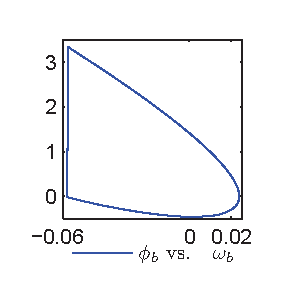
\includegraphics[width=0.24\textwidth]{pp-time-1-s}
    \label{fig:pp-t-ref}
  }
  \subfloat[Ankle angles]{
    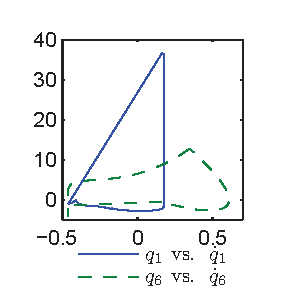
\includegraphics[width=0.24\textwidth]{pp-time-2-s}
    \label{fig:pp-t-ankle}
  }
  \subfloat[Knee angles]{
    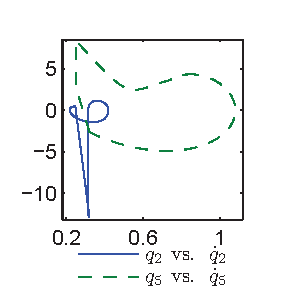
\includegraphics[width=0.24\textwidth]{pp-time-3-s}
    \label{fig:pp-t-knee}
  }
  \subfloat[Hip angles]{
    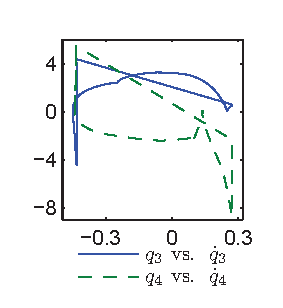
\includegraphics[width=0.24\textwidth]{pp-time-4-s}
    \label{fig:pp-t-hip}
  }
  \caption{Phase portraits of simulation of time-based system $\HS_t$.}
  \label{fig:pp-t}
\end{figure*}
%
\begin{figure}[t!]
  \centering
  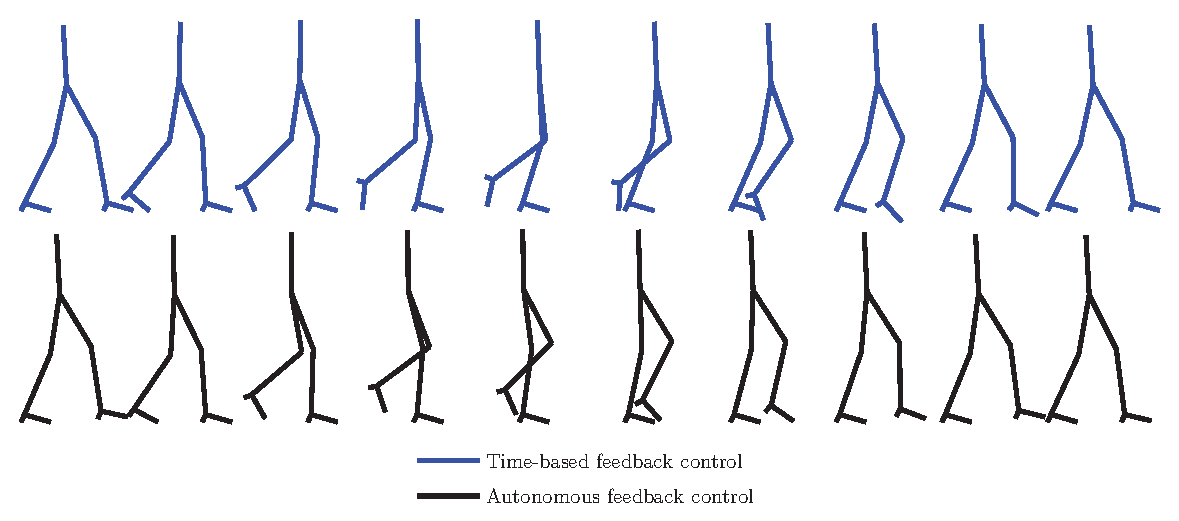
\includegraphics[width=1.0\textwidth]{hic_gait_tiles}
  \caption[Comparison of simulated walking gaits.]{Comparison of simulated
    walking gaits. Time-based feedback control and autonomous feedback
    control.}
  \label{fig:gaittiles}
\end{figure}
%
Snapshots of the walking gait are shown in \figref{fig:gaittiles}.
%
These simulation results imply that, through a choice of functions intrinsic to
human walking, humanlike walking was indeed obtained for on an anthropomorphic
biped.
%
The humanlike nature of the simulated gait can best be seen in a video of the
walking available online.\fnref{fn:rwsinnet}


\section{Autonomous Feedback Controller Design}

In general, autonomous control is preferred over non-autonomous, time-based
control as autonomous controllers tend to be more robust.
%
In this section, a method is given which shows how to remove the time-dependence
from the ``canonical'' functions described in the previous section.
%
A common trick in the literature \cite{Westervelt2007} for converting time-based
trajectories into state-based trajectories is to parameterize time by a
state-dependent function;
%
this results in an autonomous feedback control strategy.

\begin{figure}[t]
  \centering
  \subfloat[Comparison of hip movement] {
    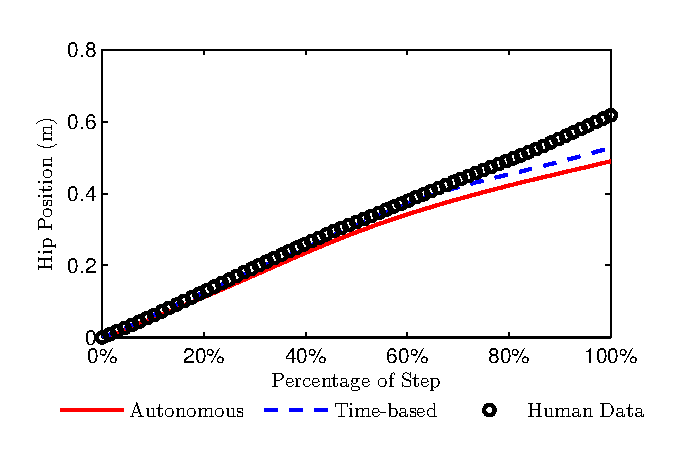
\includegraphics[width=.48\textwidth]{hip_pos}
    \label{fig:hip-pos}
  }
  \subfloat[Angular motion of torso] {
    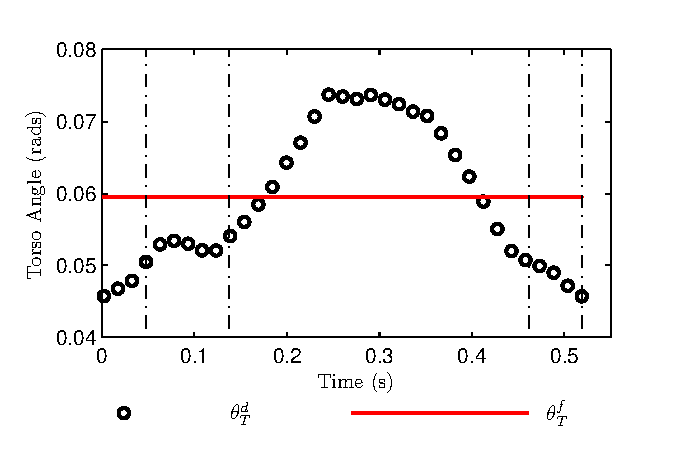
\includegraphics[width=.48\textwidth]{torso_angle}
    \label{fig:torso-angle}
  }
  \caption{Trajectories for the hip (a) and torso (b).}
  \label{fig:torso-hip}
\end{figure}


\subsection{State-Based Trajectory Parameterization}

Recall that the functions discussed in the previous section are directly
dependent on time, i.e., they can be written $y_{\vo}^{d}\argt$.
%
Furthermore, these functions are all defined on some interval $[t^{-} = 0, t^{+}
= P] = \mathcal{I} \subset \R_{0}^{+}$ with $P$ the period of the gait (that is,
one step with one leg);
%
in other words, a given tracking function can be written as a map $y_{\vo}^{d} :
\mathcal{I} \to \R$.
%
Autonomous state feedback can be achieved by simply choosing a state-based
parameterization $\varsigma : \Q \to \mathcal{I}$ and substituting for time,
i.e., $y_{\vo}^{d}(\varsigma\argsq)$.

When choosing a parameterization, $\varsigma\argsq$, it is important to consider
its role in the system.
%
Since $\varsigma\argsq$ is a parameterization for time $t$, the relationship
between $\varsigma\argsq$ and $t$ should be as linear as possible.
%
Examination of the human hip data, as shown in \figref{fig:hip-pos}, reveals
that the hip velocity $v_{\mathit{hip}}^{x}$ is constant throughout the gait;
%
as a result, the hip position approximately satisfies
$p_{\mathit{hip}}^{x}(\q\argt) = v_{\mathit{hip}}^x t + p_\mathit{hip}^x(\qm)$,
with $\qm$ the state at the beginning of a step.
%
Here, the assumption can be made, without loss of generality, that time starts
at zero at the beginning of any given step.
%
The linearity of the hip position, $p_{\mathit{hip}}^{x}(\q\argt)$, with respect
to time, makes it a good candidate for time parameterization;
%
substituting $\varsigma\argsq \to t$ and solving for $\varsigma\argsq$ gives the
parameterization
\begin{align}
  \label{eq:prm}
  \varsigma\argsq = \frac{p_{\mathit{hip}}^{x}\argsq -
    p_{\mathit{hip}}^{x}\argsqm}{v_{\mathit{hip}}^{x}}.
\end{align}
%
The parameters $p_{\mathit{hip}}^{x}\argsqm$ and $v_{\mathit{hip}}^{x}$ should be
chosen based on the quantities they represent (i.e., $v_{\mathit{hip}}^{x}$
should be the average velocity of the hip and $p_{\mathit{hip}}^{x}\argsqm$ should
be the $x$-position of the hip at the beginning of a step).
%
In this work, these values were found by examining the simulation of the
time-based controller from the previous section.
%
Specifically, a good choice for $v_{\mathit{hip}}^{x}$ is the parameter for the
hip velocity constraint, $A_{3,1}$ (found in \tabref{tab:funcparam}).
%
Using the parameterization \eqref{eq:prm}, the desired trajectories can be
expressed by substituting the parameterization $\varsigma\argsq$ for time $t$;
%
that is, the desired trajectories will be given by
$y_{\vo}^{d}(\varsigma\argsq)$.


\subsubsection{Control Design Modification}

Implementation of state feedback allows for the removal of time from the virtual
outputs, that is, the control law is no longer time-dependent.
%
Therefore, the virtual output of \eqref{eq:virtout} becomes
\begin{align*}
  y_{\vo}\argsqdq = y_{\vo}^a\argsqdq - y_{\vo}^{d}(\varsigma\argsq)
\end{align*}
with $\varsigma\argsq$ the parameterization given in \eqref{eq:prm}.
%
Following the derivation of the time-based controller, the outputs are grouped
based on relative degree:
%
\begin{align*}
  y_{\vo}\argsqdq = (y_{\vo,1}\argsqdq, y_{\vo,2}\argsq).
\end{align*}
%
The control law which drives $y_{\vo}\argsqdq \to 0$ is then given by
\begin{align*}
  \uu\argsqdq = -\mathcal{A}_{\vo}^{-1}\argsqdq \left(
  \left[ \begin{array}{c}
      0\\
      L_{\xf_{\vo}} L_{\xf_{\vo}} y_{\vo,2}\argsq
    \end{array} \right] +
  \left[ \begin{array}{c}
      L_{\xf_{\vo}} y_{\vo,1}\argsqdq\\
      2 \varepsilon L_{\xf_{\vo}} y_{\vo,2}\argsq
    \end{array} \right] +
  \left[ \begin{array}{c}
      \varepsilon y_{\vo,1}\argsqdq\\
      \varepsilon^2 y_{\vo,2}\argsq
    \end{array} \right]\right),
\end{align*}
with $A_{\vo}(q)$ the decoupling matrix given by
\begin{align}
  \mathcal{A}_{\vo}\argsqdq =
  \left[\begin{array}{c}
      L_{\xg_{\vo}} y_{\vo,1} \argsqdq\\
      L_{\xg_{\vo}} L_{\xf_{\vo}} y_{{\vo},2}\argsq
    \end{array}\right]
\end{align}
and $(\xf_{\vo}, \, \xg_{\vo})$ the control system given in
\eqref{eq:controlsystem}.
%
Application of this control law to the control system yields the closed-loop
system:
%
\begin{align}
  \xf_{cl,\vo} = \xf_{\vo}\argsqdq + \xg_{\vo}\argsq \, \uu\argsqdq.
\end{align}
%
The virtual outputs are chosen to be the same as those in the time-based
controller, specified in \tabref{tab:fitcor}.
%
The end result is an autonomous hybrid system specified by
\begin{align}
  \HS_{a} = (\Gamma, \, \D, \, \Guard, \, \Delta, \, \F_{a}).
\end{align}
with $\F_{a}$ the set of vector fields $\{\xf_{cl,\vo}\}_{\vo \in V}$.


\begin{figure*}[tp!]
  \centering
  \subfloat[Body frame angle]{
    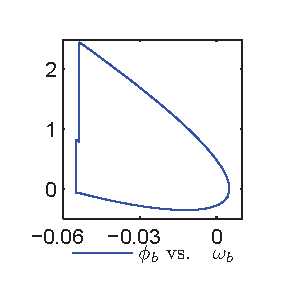
\includegraphics[width=0.24\textwidth]{pp-auto-1-s}
    \label{fig:pp-a-ref}
  }
  \subfloat[Ankle angles]{
    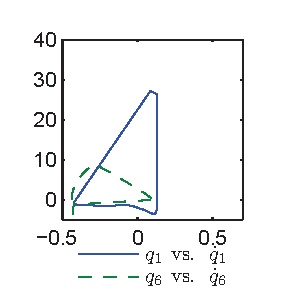
\includegraphics[width=0.24\textwidth]{pp-auto-2-s}
    \label{fig:pp-a-ankles}
  }
  \subfloat[Knee angles]{
    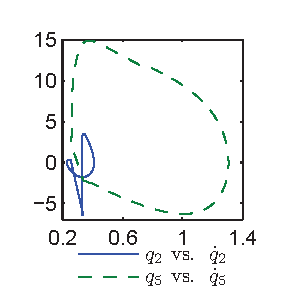
\includegraphics[width=0.24\textwidth]{pp-auto-3-s}
    \label{fig:pp-a-knee}
  }
  \subfloat[Hip angles]{
    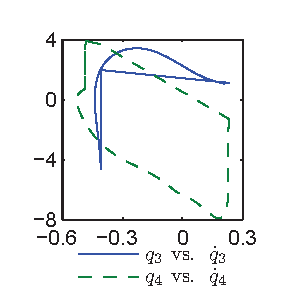
\includegraphics[width=0.24\textwidth]{pp-auto-4-s}
    \label{fig:pp-a-hip}
  }
  \caption{Phase portraits of simulation of autonomous system $\HS_{a}$.}
  \label{fig:pp-a}
\end{figure*} 


\subsection{Simulation of Autonomous Feedback Controller}

The analysis of the stability of the autonomous system is analogous to that
shown in \secref{sec:timesim}.
%
The control gain is again chosen to be $\varepsilon = 15$.
%
The parameters are tweaked, as before, by multiplying row six by $1.25$.
%
This simulation results in the fixed point:
%
\begin{align*}
  \qst_{s,t} &=
  \left(\begin{array}{r r r r r r}
      -\hphantom{1}.404 & .245 & \hphantom{1}.208 & -\hphantom{0}.488 &
      \hphantom{-2}.388 & \hphantom{-}.088
  \end{array}\right)\\
  \dqst_{s,t} &=
  \left(\begin{array}{r r r r r r}
    -1.287 & .282 & 1.078 & \hphantom{-}0.711 & -2.452 & -.076
  \end{array}\right)
\end{align*}
on the guard of domain {\DC}.
%
Only the shape coordinates are shown, as in the analysis of the time-based
feedback controller.
%
The Jacobian matrix of a linearization of the \Poincare{} map about the fixed
point $(\qst_{s}, \dqst_{s})$ yields eigenvalues of the following
magnitudes:
%
\begin{align*}
  |\lambda_{a}| \in \{0.1902, \, 0.0680, \, 0.0680, \, 0.504, \, 0.0058, \,
  \ldots\},
\end{align*}
where, again, only the five eigenvalues with the largest magnitudes are shown.
%
The phase portraits are shown in \figref{fig:pp-a}.

%\chapter{\uppercase{Functional Routhian Reduction}}

Classical Routhian reduction \cite{} is a method which takes advantages of symmetries inherent in a dynamical system and utilizes conserved momentum to eliminate cyclic variables, thereby reducing the dimensionality of the system and simplifying controller design. Functional Routhian reduction (first introduced in \cite{}) is a variant in which the conserved momentum is set to a function rather than a constant. This scheme has enjoyed success in migrating 2D gaits to 3D. By decoupling the sagittal and coronal dynamics, functional Routhian reduction provides insight into the decoupled nature of human walking and allows for sagittal control design to be conducted on a reduced-order model while simultaneously providing coronal stabilization. This remarkable relationship between dynamics, while only providing a slight reduction in dimensionality, shifts the control problem from designing complicated 3D walking gaits to the much more tractable challenge of designing 2D gaits. Thus, stable walking is obtained in 3D by simply applying control laws which give stable walking in the sagittally-restricted counterpart in 2D (which has a Lagrangian of the form given in \eqref{}).


\section{Almost-Cyclic Lagrangians}
Consider a system with configuration space $\Q = \Shape \times \T$, where $\Shape$ is called the shape space. Let the coordinates be represented by $\q = (\varphi^T, \theta^T)^T$ with $\theta \in \Shape$ and almost-cyclic variable $\varphi \in \mathbb{T}^{\ncv}$. A Lagrangian $\Lag_{\lambda} : T\Shape \times T\T \to \R$ is almost-cyclic if it takes the form in \eqref{} from \cite{} for some $\lambda : \T \to \R$.

\section{Momentum Maps}
As alluded to earlier, functional Routhian reduction utilizes a momentum map, $J : T\Q \to \R$, which specifies conserved quantities:
\begin{align*}
  J(\varphi, \theta, \dot \varphi, \dot \theta) = 
\end{align*}
This map is equal to a function, $\lambda(\varphi)$.

\section{Functional Routhians}

\section{Reduction Theorem}

\chapter{\uppercase{Simulation Results}} \label{chap:simulations}

This chapter provides example systems to help provide intuition into energy
shaping procedures and to demonstrate the outcome of applying energy shaping to
these example systems.
% 
Four examples are covered and they are arranged by complexity.
% 
The first example covered is the cart--spring system, which is a
single--degree-of-freedom system.
% 
This example is, perhaps, the most informative due its simplicity:
% 
with one degree-of-freedom, it is possible to provide figures demonstrating the
domain of attraction and to plot a proper phase portrait.
% 
The next example is the compass-gait biped walking down a shallow slope.
% 
This system which is motivated largely by McGeer's work \cite{McGeer1990} has
two degrees-of-freedom and exhibits conservation of energy in the continuous
dynamics.
% 
The third system is a three-link biped with a torso walking on flat ground under
the influence of \cs \cite{Spong2005} and additional
non-conservative forcing.
% 
The fourth and final system is a seven-link, multi-domain biped which uses a
number of controllers to achieve walking.
% 
This model is rather complex in comparison to the other examples and is provided
primarily to demonstrate energy shaping on multi-domain hybrid systems.

In addition to verifying the formal results guaranteed by
\thmref{theorem:main-theorem}, this chapter will also attempt to provide some
substance to the claims made about the benefits of energy shaping.
% 
It was loosely mentioned that energy shaping can be used to improve robustness
of systems with respect to perturbations in initial conditions.
% 
Although it may be possible to demonstrate the domain of attraction for some
models, doing so requires the explicit construction of a Lyapunov function.
% 
And though \thmref{theorem:main-theorem} guarantees the implicit existence of a
valid Lyapunov function by fulfilling the necessary conditions for Lyapunov's
direct method (converse Lyapunov theorem), it does not provide the explicit
function in much the same way as the definition of time-to-impact as an implicit
function does not provide any clue as to its explicit form.
% 
As a result and because of the difficulty of guessing a Lyapunov function, 




\begin{figure}[t!]
  \centering
  \def\svgwidth{0.7\columnwidth}
  \input{figs/cart_spring.eps_latex}
  \caption[Configuration of the cart--spring system.]{Configuration of the
    cart--spring system. Values used in simulation shown in \tabref{tab:cart_spring_parameters}.}
  \label{fig:cart-spring-configuration}
\end{figure}

\begin{table}[t!]
  \caption{Physical parameters for the cart--spring simulation.}
  \label{tab:cart_spring_parameters}
  \centering
  \begin{tabular}{c c c}
    $M = 1 \ \mathrm{kg},$ &
    $K = 1 \ \mathrm{N/m},$ &
    $\gamma = .2 \ \mathrm{kg/m^{2}/s}$
  \end{tabular}
  \vspace{-1em}
\end{table}

\section{Cart--Spring System}\label{sec:cart_spring}

The simplest example system to which energy shaping can be applied is a system
with a one-dimensional configuration space.
% 
The cart--spring system shown in \figref{fig:cart-spring-configuration} (with
simulation parameters given in \tabref{tab:cart_spring_parameters}) is just such
a system and can be used to build intuition into the methods presented.

\subsection{Setup}

This well-known example is highly idealized and assumes rolling without slipping
and no damping.
% 
As shown in \figref{fig:cart-spring-configuration}, the cart has mass $M$ and is
acted on by an idealized spring with stiffness $K$.
% 
It is assumed that (by turning the wheels) a force can be applied directly along
the $x$-axis in the same way in which the spring acts.

% 
Parameterizing the motion of the system by the horizontal displacement, $\q$, with
associated velocity $\dq$, leads to the configuration space $\Q = \R$ with
tangent bundle $T\Q = \R^{2}$ which has coordinates $\x = \argsqdq \in \T\Q$.
% 
Disregarding physical restrictions on spring length leads to the domain of
admissibility for the system being entire, i.e.,
\begin{align*}
  \D = \R^{2}.
\end{align*}
% 
The dynamics of the system obeys the differential equation
\begin{align*}
  M \ddq + K \q = \uu
\end{align*}
where $M$ is the mass of the cart, $K$ is the spring constant, and $u$ is the
control force in newtons.

This system is not intrinsically a hybrid system and, as a result, energy
shaping cannot be directly applied.
% 
However, this system can be made amenable to energy shaping by embedding it
in a hybrid system.
% 
Consider that the motion of the cart--spring system involves oscillation about
the origin.
% 
Thus all non-trivial trajectories pass through the origin repeatedly, so a
natural choice for the switching surface (\Poincare{} section) is the set
\begin{align}
  \Guard = \left\{ \argsqdq \in T\Q : \q = 0 \mbox{ and } \dq < 0 \right\}.
  \label{eq:cart_spring_guard}
\end{align}
% 
Using this switching surface with the domain of admissibility specified above
permits reformulation of the cart--spring system as a hybrid system:
% 
\begin{align}
  \HCS = \left\{
    \begin{array}{l l}
      \dx\hphantom{^+} = \xf\argsqdq + \xg \, \uu, & \argsqmdqm \in \D \setminus
      \Guard,\\
      \xp = \argsqmdqm, & \argsqmdqm \in \Guard,
    \end{array}\right.
\end{align}
where
\begin{align*}
  \xf\argsqdq = \left(\begin{array}{c}
      \dq\\
      -\frac{K}{M} \q
    \end{array}\right), \qquad
  \xg = \left(\begin{array}{c}
      0\\
      \frac{1}{M}.
    \end{array}\right).
\end{align*}

For the constructed hybrid system, the discrete dynamics do not have any effect
on the configuration and velocity; in other words, the discrete dynamics is the
identity map.
% 
Moreover, with no control input, the system is conservative and does not exhibit
asymptotic stability.
% 
In order to demonstrate the application of energy shaping, a limit cycle can be
induced in the system using, for example, the same dissipation present in the
Van der Pol oscillator (see \cite[pp.~13]{Khalil2002}).
% 
As described in \chapref{ch:energy-shaping}, the state of the system can be
augmented to include a storage function for energy flow due to non-conservative
forcing, i.e.,
\begin{align*}
  \x = \argsqdqW
\end{align*}
where $\W$ is an energy storage function as in \eqref{eq:storage-function-Fnc}.
% 
Applying the feedback control law
\begin{align}
  \label{eq:spring_cart_vdp_controller}
  \uu = \vv\argsqdq = \gamma(1 - \q^{2}) \, \dq + w
\end{align}
with $\gamma \in \Rnn$ leads to the hybrid control system
\begin{align}
  \label{eq:hcs_cart_spring}
  \HCSbar = \left\{
    \begin{array}{l l}
      \dx\hphantom{^+} = \xfbar\argsqdq + \xgbar \, w, & \argsqmdqm \in \D \setminus \Guard,\\
      \xp = \Delta\argsqmdqm, & \argsqmdqm \in \Guard,
    \end{array}\right.
\end{align}
where the nominal controller is subsumed under the system dynamics and energy
flow is tracked in the $W$ coordinate, viz.
\begin{align}
  \label{eq:FGbar_cart_spring}
  \xfbar\argsqdq = \left(\begin{array}{c}
      \dq\\
      -\frac{K}{M} \q + \frac{1}{M} \gamma(1 - \q^{2}) \, \dq\\
      \gamma(1 - \q^{2}) \, \dq^{2}
    \end{array}\right), \qquad
  \xgbar\argsdq = \left(\begin{array}{c}
      0\\
      \frac{1}{M}\\
      0
    \end{array}\right),
\end{align}
and the reset map acts to reset the stored energy, i.e.,
\begin{align*}
  \Delta\argsqdq = (\q, \dq, 0).
\end{align*}
% 
The hybrid control system \eqref{eq:hcs_cart_spring} is of the same form as
\eqref{eq:hcs_bar} but is written in a more compact way.


\begin{figure*}[htp!]
  \centering
  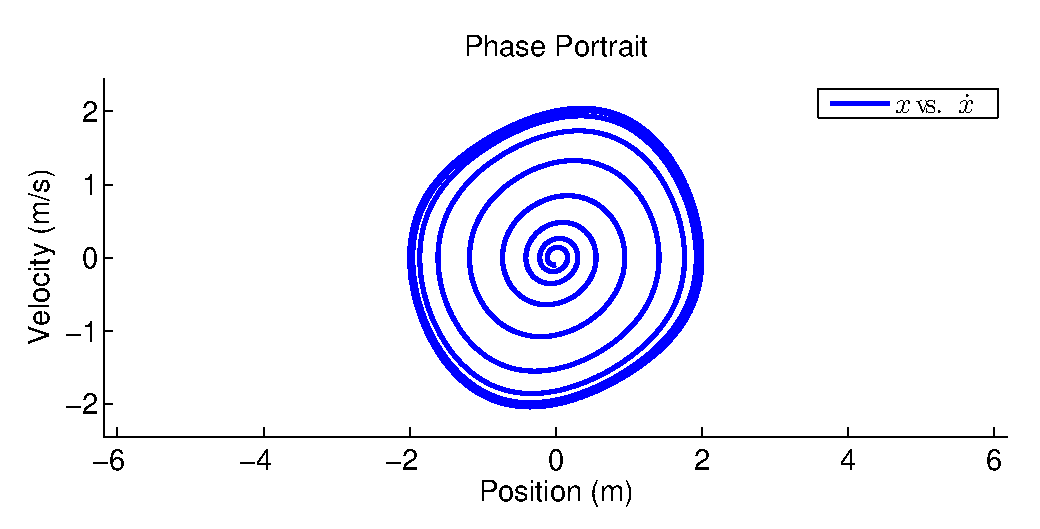
\includegraphics[width=0.85\textwidth]{hybrid_cart_spring_phase_portrait}
  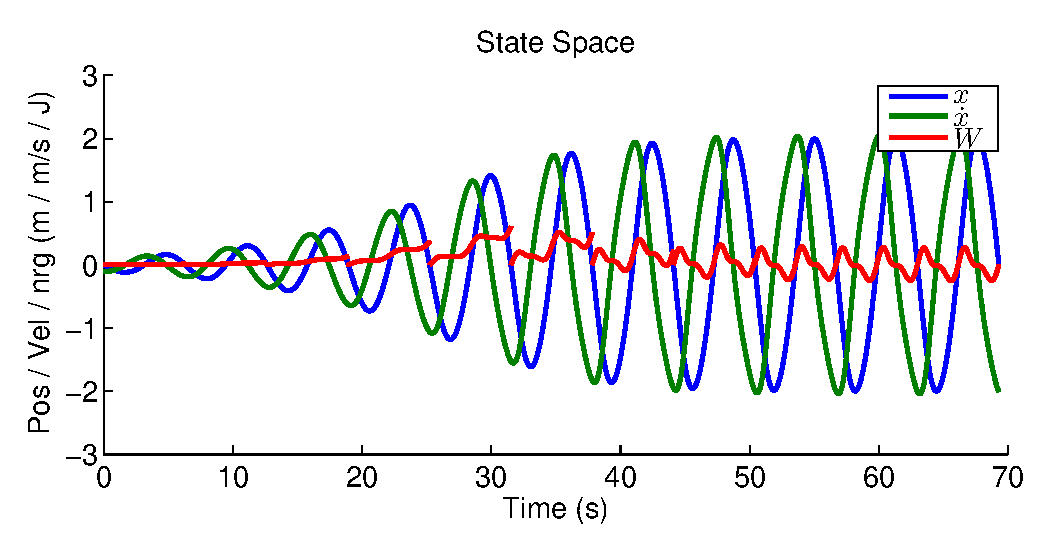
\includegraphics[width=0.85\textwidth]{hybrid_cart_spring_coordinates}
  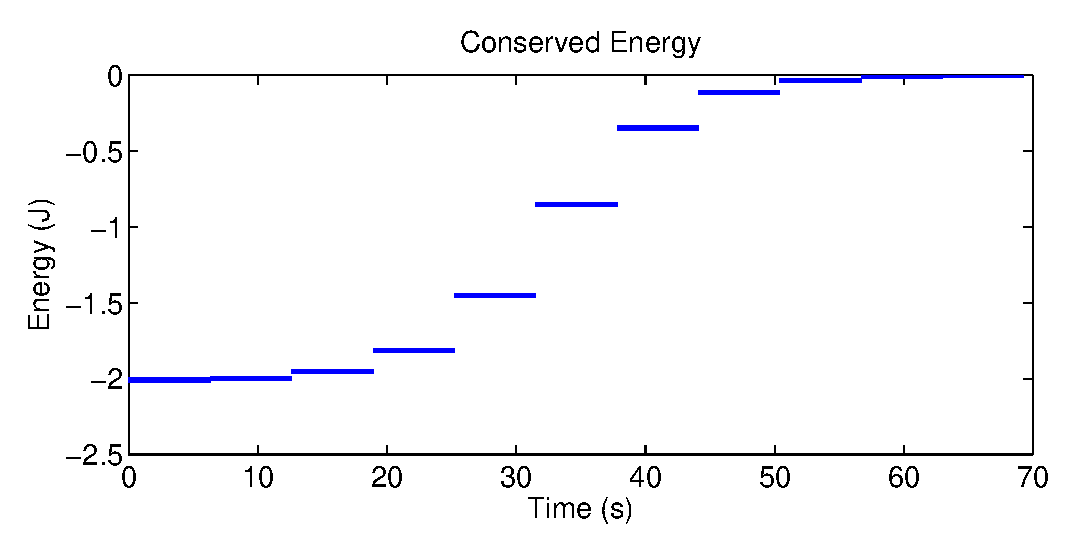
\includegraphics[width=0.85\textwidth]{hybrid_cart_spring_energy}
  \caption[Simulation of the nominal cart--spring system.]{Simulation of the
    nominal cart--spring system.
    % 
    A force from the nominal control law \eqref{eq:spring_cart_vdp_controller}
    acts on the cart.
    % 
    Top: phase portrait demonstrating the existence of a limit cycle;
    % 
    middle: evolution of the state coordinates;
    % 
    bottom: the conserved energy jumps when the storage function is reset at the
    switching surface.}
  \label{fig:cart_spring_simulation_nominal}
\end{figure*}


\subsection{Simulation of Nominal System}
Beginning from the (post-reset) initial condition
\begin{align*}
  \argsqdqW = (0, -.1, 0),
\end{align*}
a simulation was conducted to illustrate the nominal behavior of cart--spring
system governed by \eqref{eq:hcs_cart_spring} and \eqref{eq:FGbar_cart_spring}
under influence of the Van der Pol controller defined in
\eqref{eq:spring_cart_vdp_controller} with $w = 0$;
% 
that is, the closed-loop hybrid system
\begin{align}
  \label{eq:hs_cart_spring_nominal}
  \HSbar = \left\{
    \begin{array}{l l}
      \dx\hphantom{^+} = \xfbar\argsqdq, & \argsqmdqm \in \D \setminus \Guard,\\
      \xp = \Delta\argsqmdqm, & \argsqmdqm \in \Guard,
    \end{array}\right.
\end{align}
% 
The parameters used are given in \tabref{tab:cart_spring_parameters}; two of the
parameters refer to the mass and spring constant as shown in \figref{fig:cart-spring-configuration}.
% 
The simulation was designed to terminate when the distance between successive
crossings of the \Poincare{} section \eqref{eq:cart_spring_guard} dropped below
a threshold---in this case, $10^{-3}$---thus serving as the convergence
criterion.
% 
Mathematically, this convergence criterion can be expressed as
\begin{align}
  \label{eq:cart_spring_convergence}
  \P_{\TI\arx}\arx - \x < 10^{-3}, \quad \x \in \Guard.
\end{align}
% 
In this case, the distance metric is the standard Euclidean one and involves
only the velocity coordinate due to the definition of the \Poincare{} section
\eqref{eq:cart_spring_guard}.

From \figref{fig:cart_spring_simulation_nominal}, it is apparent that the
simulation lasted just under $70$ seconds.
% 
The phase portrait in \figref{fig:cart_spring_simulation_nominal} shows that the
system eventually converges to a limit cycle over relatively large number of
steps (i.e., iterations of the \Poincare{} first return map).
By counting the jumps in the plot of conserved energy in
\figref{fig:cart_spring_simulation_nominal}, one can see that convergence based
on the aforementioned criterion requires 11 ``steps'';
% 
in other words, the cart passes through the origin from the positive side 11
times.


From the evolution of the coordinates shown in
\figref{fig:cart_spring_simulation_nominal}, it is apparent that the
oscillations grow until the system reaches the limit cycle.
% 
The conserved energy of the limit cycle (as defined in
\eqref{eq:ncsys-nrg-cons} and \eqref{eq:storage-function-Fnc}) can be seen to change between iterations in \figref{fig:cart_spring_simulation_nominal}.
% 
This jump is a result of the resetting of the storage function, $W$, which
occurs when the cart passes through the switching surface
\eqref{eq:cart_spring_guard}.

\subsection{Simulation of Shaped System}

To demonstrate the effect of energy shaping, a simulation was conducted on the
cart--spring system described in the previous subsection.
% 
The relevant hybrid control system for the application of energy shaping is
given in \eqref{eq:hcs_cart_spring} and \eqref{eq:FGbar_cart_spring}.
% 
In contrast to the nominal simulation, this simulation was conducted with $w$
given by the min-norm control law \eqref{eq:min-norm} designed to satisfy the
conditions of energy shaping \eqref{eq:es-qp}, which results in the
hybrid system
\begin{align}
  \label{eq:hs_cart_spring_es}
  \HSbar = \left\{
    \begin{array}{l l}
      \dx\hphantom{^+} = \xfbar\argsqdq + \xgbar \, \mueps\argsqdqW, & \argsqmdqm \in \D \setminus \Guard,\\
      \xp = \Delta\argsqmdqm, & \argsqmdqm \in \Guard,
    \end{array}\right.
\end{align}
with $\xfbar$ and $\xgbar$ as given in \eqref{eq:FGbar_cart_spring}.

The results of the simulation of \eqref{eq:hs_cart_spring_es} are shown in
\figref{fig:cart_spring_simulation_shaped}.
% 
Like the simulation of the nominal system, this simulation of the shaped system
\eqref{eq:hs_cart_spring_es} was designed to terminate upon convergence using
the same criterion as specified in \eqref{eq:cart_spring_convergence}.
% 
From this figure, it is immediately obvious that convergence occurs in fewer
steps than for the nominal simulation;
% 
for this shaped simulation, convergence requires three steps (count the
zero-crossings of $q$ in the middle plot of
\figref{fig:cart_spring_simulation_shaped}) and the simulation lasted under 20
seconds.
% 
In addition, it is apparent from the phase portrait that the convergence happens
very rapidly.
% 
The speed of convergence can be affected by varying the gain $\resclfparam$ of
the energy shaping controller \eqref{eq:es-qp}.

These numerical simulations show that energy shaping can provide improved
convergence properties for stable systems.
% 
However, because the Van der Pol controller is globally stable, it is not
possible to demonstrate an increase in domain of attraction;
% 
this benefit of energy shaping will be shown in the next example.


\begin{figure*}[htp!]
  \centering
  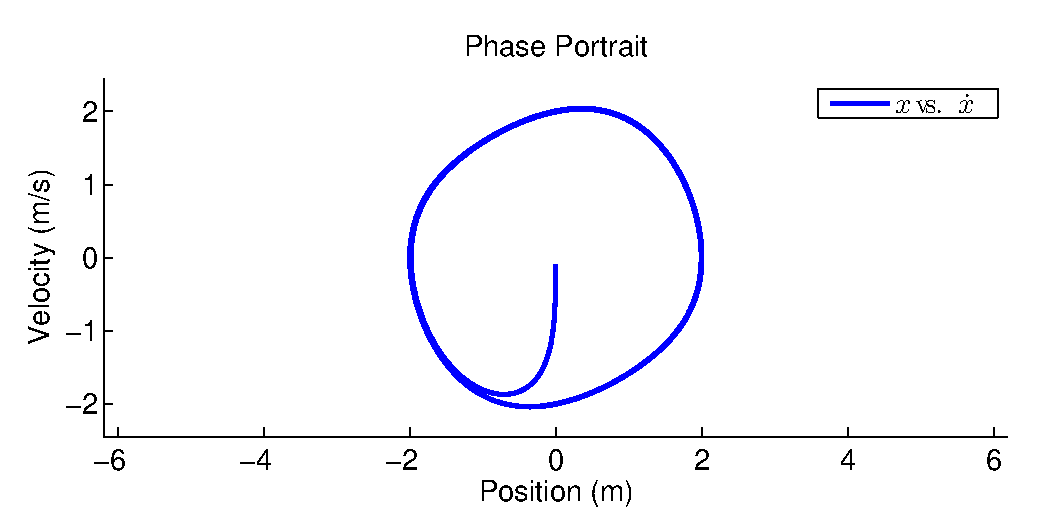
\includegraphics[width=0.85\textwidth]{hybrid_cart_spring_es_phase_portrait}
  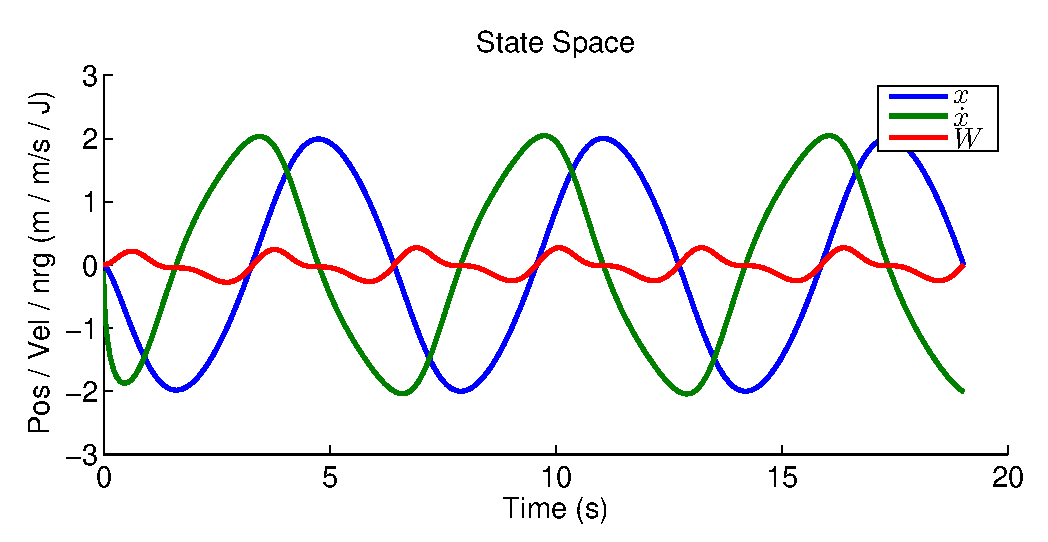
\includegraphics[width=0.85\textwidth]{hybrid_cart_spring_es_coordinates}
  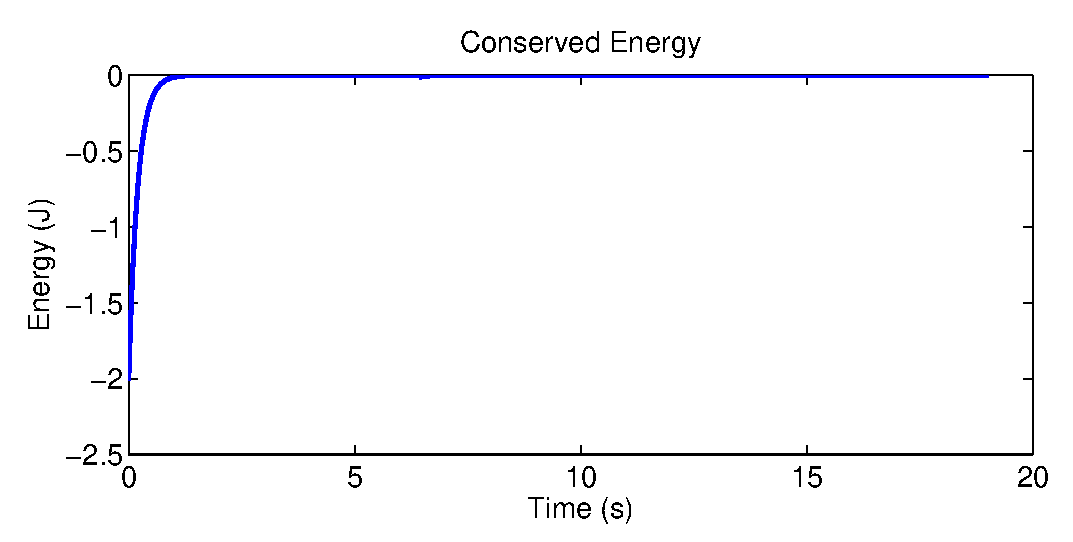
\includegraphics[width=0.85\textwidth]{hybrid_cart_spring_es_energy}
  \caption[Simulation of the shaped cart--spring system.]{Simulation of the
    shaped cart--spring system.
    % 
    A force from the nominal control law \eqref{eq:spring_cart_vdp_controller}
    acts on the cart along with a force from energy shaping.
    % 
    Top: phase portrait demonstrating the existence of a limit cycle and rapid
    stabilization;
    % 
    middle: evolution of the state coordinates;
    % 
    bottom: the conserved energy stabilizes to the desired value at an
    exponential rate.}
  \label{fig:cart_spring_simulation_shaped}
\end{figure*}


\begin{figure}
  \centering
  \def\svgwidth{0.5\columnwidth}
  \input{figs/cg2d-slope-model.eps_latex}
  \caption{Compass-gait biped with walking down a slope.}
  \label{fig:simulation-model}
  \vspace{-1em}
\end{figure}

\begin{table}[t]
  \caption{Physical parameters for the simulation model.}
  \label{tab:mparam}
  \centering
  \begin{tabular}{c c c c}
    $M =20 \ \mathrm{kg},$ &
    $m = 5 \ \mathrm{kg},$ &
    $\ell = 1 \ \mathrm{m},$ &
    $\gamma = .05 \ \mathrm{rads}$
  \end{tabular}
  \vspace{-1em}
\end{table}

\section{Compass-Gait Biped} \label{sec:simulations-compass-gait}

\begin{figure}[p!]
  \centering
  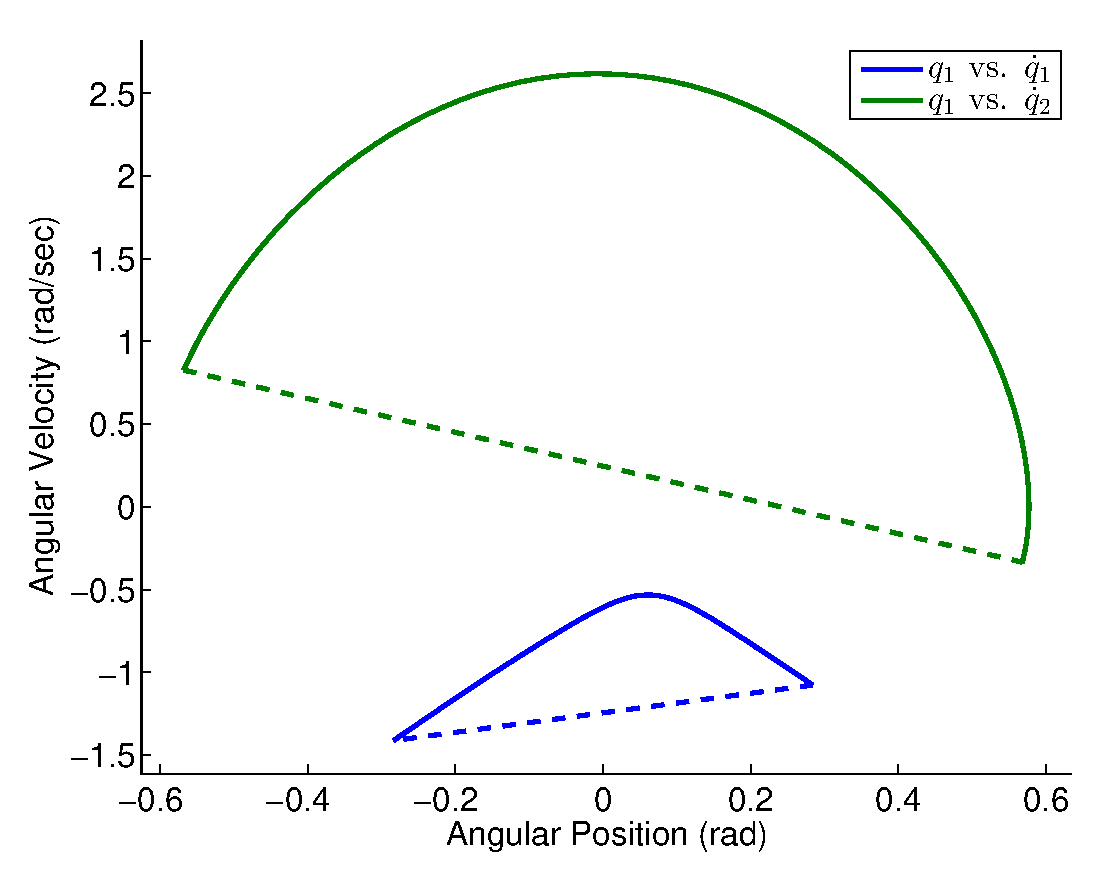
\includegraphics[width=0.75\columnwidth]{cg-limit-cycle}
  \caption{Limit cycle of the passive compass gait biped.}
  \label{fig:lc}
\end{figure}

\begin{figure}[p!]
  \centering
  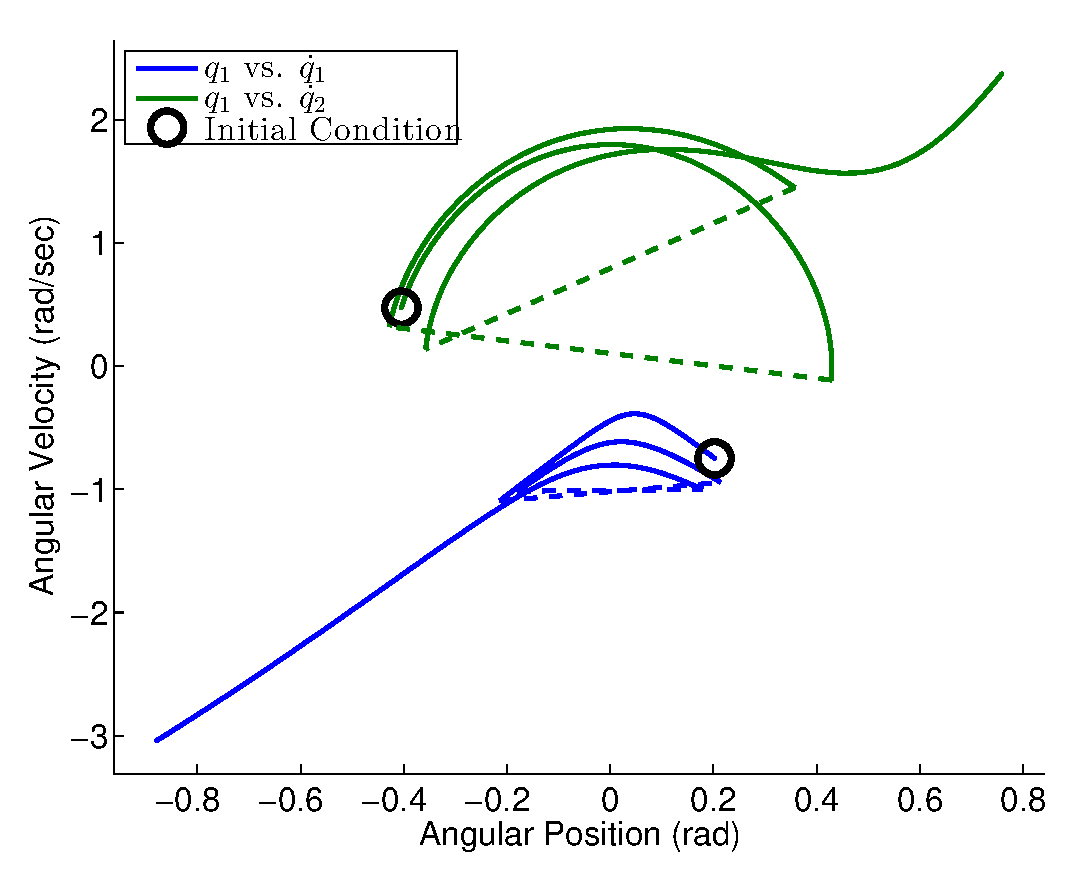
\includegraphics[width=0.75\columnwidth]{cg-pp-fall}
  \caption{The passive system cannot recover from distant states.}
  \label{fig:pp-fall}
\end{figure}

With slightly greater complexity than the cart--spring system described in
\secref{sec:cart_spring}, the compass-gait biped is a two-link rigid kinematic
chain with periodic impacts (foot-strike) which cause instantaneous jumps in the
velocity coordinates.

Using the compass-gait biped model shown in \figref{fig:simulation-model} with
parameters as shown in \tabref{tab:mparam}, simulations were conducted to
demonstrate the effectiveness of the energy shaping procedure.
% 
The limit cycle of the passive system is shown in \figref{fig:lc} with the
dotted lines representing discrete jumps from foot-strike (and coordinate
relabeling).
% 
This gait has a fixed point
% 
\begin{align}
  \label{eq:fixed-point}
  (\qst, \ \dqst) = (-0.2891, \ 0.5781, \ -1.4006, \ -0.2802)
\end{align}
% 
on the guard with eigenvalues
% 
\begin{align}
  |\lambda| = (0.5147, \ 0.5147, \ 0.0980)
\end{align}
% 
corresponding to a linearization of the \Poincare{} map restricted to the guard.
% 
Due to the restriction to the guard, the \Poincare{} section is a
codimension-one hyperplane and is thus characterized with fewer coordinates (one
fewer).
% 
Because these eigenvalues have magnitude below unity, the corresponding hybrid
periodic orbit is locally exponentially stable.
% 
The impact map can be applied to the fixed point \eqref{eq:fixed-point} to
compute the post-impact coordinates
% 
\begin{align}
  \label{eq:fixed-point-post-impact}
  \Delta(\qst, \ \dqst) = (0.2891, \ -0.5781, \ -1.0681, \ 0.6797).
\end{align}

To see the benefit of energy shaping, consider two simulations conducted from a
perturbed post-impact initial condition,
% 
\begin{align}
  \label{eq:ic-sim-1}
  (\q_{0}, \ \dq_{0}) = (0.2023, \ -0.4047, \ -0.7477, \ 0.4758),
\end{align}
% 
which was naively obtained by multiplying the post-impact fixed point
\eqref{eq:fixed-point-post-impact} by $0.7$ resulting in a relatively large
perturbation.
% 
For the passive walker, one can see from \figref{fig:pp-fall} that the biped
falls on the third step.
% 
When energy shapping is added by choosing $\frac{c_{3}}{\resclfparam} = 1$ as in
\figref{fig:pp-recover}, the biped is able to recover from the same initial
condition and quickly converges to the limit cycle.
% 

\begin{figure}[p!]
  \centering
  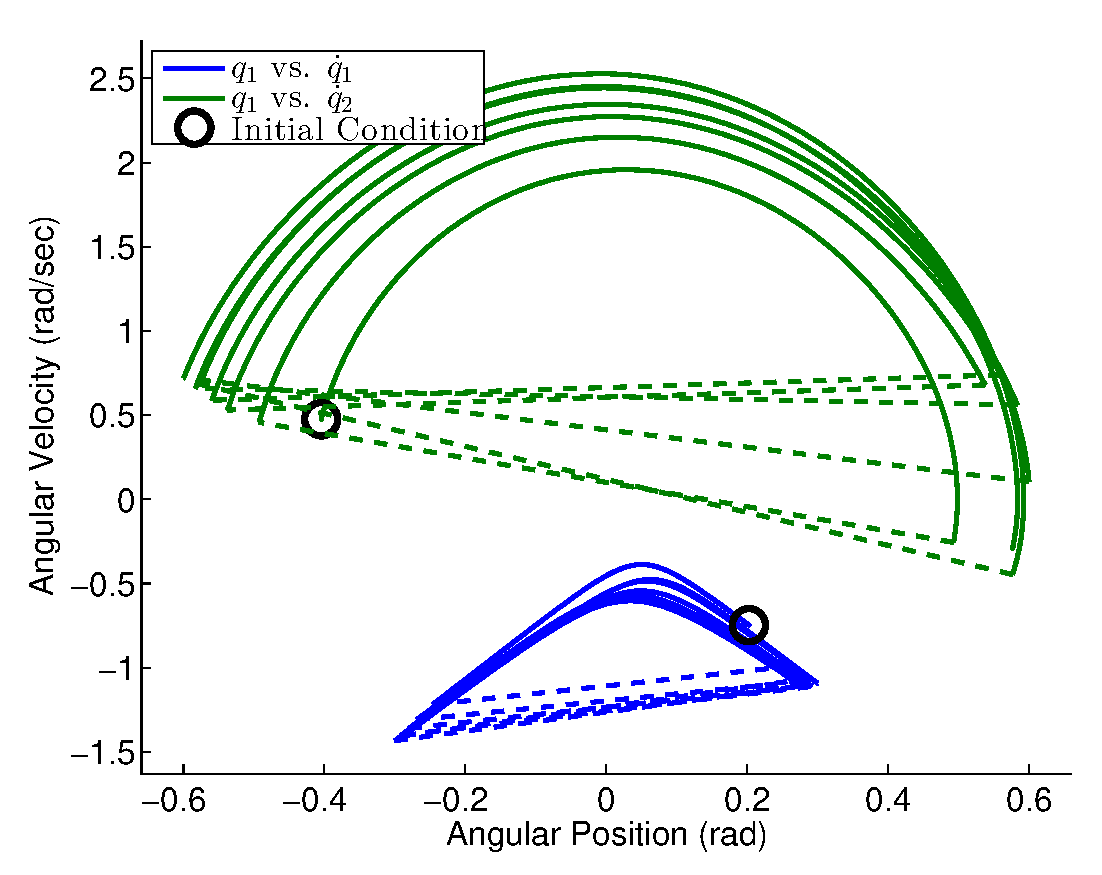
\includegraphics[width=0.75\columnwidth]{cg-pp-recover}
  \caption{Energy shaping allows recovery from more distant states.}
  \label{fig:pp-recover}
\end{figure}

\begin{figure}[p!]
  \centering 
  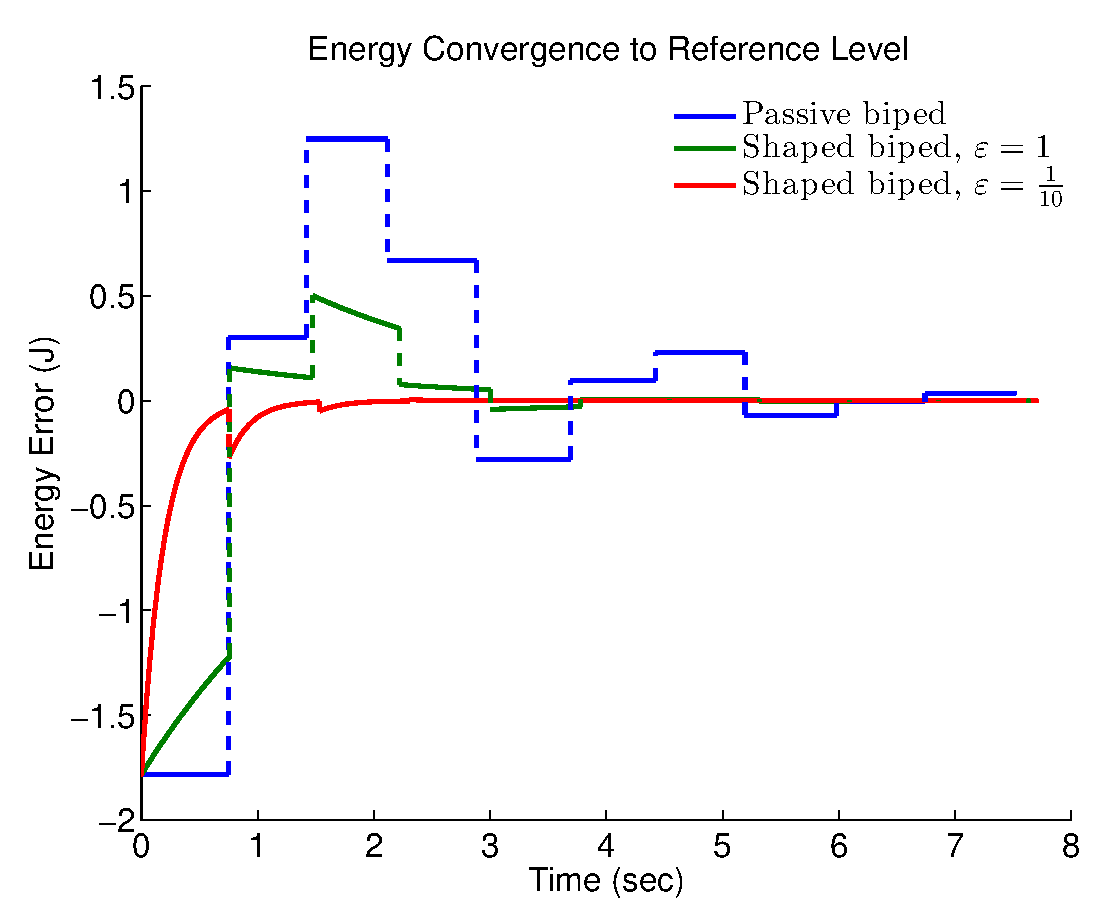
\includegraphics[width=0.75\columnwidth]{cg-energy-comp}
  \caption[Convergence has more desirable behavior with energy
  shaping.]{Convergence has more desirable behavior with energy shaping. Smaller
    values of $\resclfparam$ offer better convergence.}
  \label{fig:energy-comp}
  \vspace{-1em}
\end{figure}

In addition to the ostensible increase in robustness, energy shaping also seems
to improve convergence properties.
% 
To see this, a simulation was conducted from the starting point
% 
\begin{align}
  (\q_{0}, \ \dq_{0}) = (0.2457, \ -0.4914, \ -0.9079, \ 0.5777),
\end{align}
% 
which, in similarity to the previous simulation, was obtained by multiplying \eqref{eq:fixed-point-post-impact} by $0.85$.
% 
This point had to be closer than \eqref{eq:ic-sim-1} in order to fall within the domain of attraction (DOA) of the passive biped.
% 
The difference in convergence for the energy levels of the passive and shaped
systems is shown in  \figref{fig:energy-comp}.
% 
One can see that the shaped system converges more quickly than the passive
system.
% 
Whereas the passive system changes energy only through impact, the shaped system
also converges during the continuous dynamics.
% 
Finally, it seems, stability is mainted for large values of $\resclfparam$,
smaller values will result in better convergence so a trade-off naturally
arises.


\begin{figure}[t!]
  \centering
  \centering
  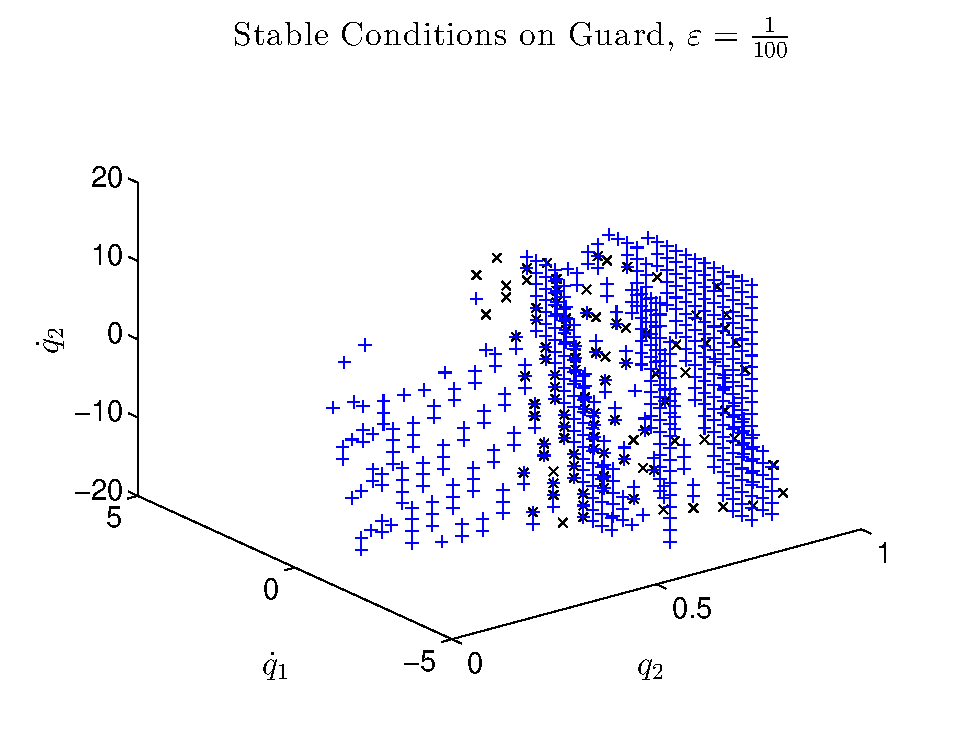
\includegraphics[width=0.75\columnwidth]{cg-poincare-cloud}
  \caption[The domain of attraction restricted to the guard.]{The domain of
    attraction restricted to the guard.
    % 
    The DOA can be viewed in three dimensions with careful scrutiny.
    % 
    The blue ``+'' symbols represent stable points of the shaped system and the
    black ``x'' symbols represents stable points of the passive system.}
  \label{fig:point-cloud}
  \vspace{-1em}
\end{figure}

More comprehensive evidence for the expansion of the domain of attraction can be
seen in \figref{fig:point-cloud} which provides a comparison of the stable
region on the guard for both the passive and shaped systems.
% 
It is interesting to note that the domain of attraction expands most readily
into the region of low energy (small steps, small angular velocities) for which
states the passive biped would simply lack the energy necessary to fall into a
gait.

\section{Seven-Link Biped}

\begin{figure}
  \centering
  \def\svgwidth{0.5\columnwidth}
  \input{figs/cg2d-7link-model.eps_latex}
  \caption{Seven-link biped configuration.}
\end{figure}

\begin{table}[t!]
  \begin{center}
    \caption[Physical model parameters of the seven-link biped.]{Physical model
      parameters of the seven-link biped. Masses and lengths are given in
      kilograms and meters, respectively.}
    \label{tab:reduction:model-parameters}
    \begin{tabular}{|c|c|c|c|c|c|}
      \hline
      $M$ & $m_{t}$ & $m_{c}$ &
      $m_{f}$ & $w_{f}$ & $w$\\
      \hline
      20 & 5 & 1 & .1 & .08 & .10 \\
      \hline
    \end{tabular}\\[.1em]
    \begin{tabular}{|c|c|c|c|c|c|c|c|c|}
      \hline
      $\ell$ & $\ell_{t}$ & $\ell_{c}$ &
      $r_{a}$ & $r_{f}$ & $r_{h}$ & $r_{t}$ & $r_{T} $\\
      \hline
      1 & .175 & .375 & .1 & .139 & .0625 & .25 & .075\\
      \hline
    \end{tabular}
  \end{center}
\end{table}


\subsection{Domain Structure}

By convention, the phases are numbered such that the transition from the last
domain to the first domain (i.e., $4 \to 1$) corresponds to heel strike as this
event signifies that the stance and swing legs should be swapped.\todo{Finish
  this section.}\xspace
% 
For the proper choice of gains, the walking controllers applied in this example
can generate a gait for which the hybrid dynamics $h_{1}(\q) = p_{stt}^{z}(\q)$,
where $p_{stt}^{z}(\q)$ is height of the stance toe above the ground, can be
combined to construct the constraint vector $H_{1}(\q, \dq, u)$. 
% 
After impact, it is desired that the stance knee be locked, that the stance foot
be flat on the ground, and that the swing toe remain fixed to the ground.
% 
These requirements dictate an apropos choice of kinematic constraints for
constructing a Jacobian for the impact map \eqref{eq:impact-model}.
% 
Using toe strike as the transition leads to the switching surface
$\GuardTransition{1}{2}$ given in \eqref{eq:guard}.
% 

\subsubsection{Phase 2 -- Toe Lift ($\DB$).}
% 
As the stance foot experiences heel roll from the previous phase and the toe
rolls into the ground causing an impact, the stance foot enters a state of flat
foot contact while the swing toe remains on the ground.
% 
The system continues under these conditions until the vertical constraining
force on the back (swing) toe reaches zero, at which point, the ground is no
longer undergoing a force interaction with the toe.
% 
This force thus represents a non-holonomic constraint on the system which can be
used to define both the switching surface and domain of admissibility (which
must always be checked).
% 
As the force reaches zero, the toe leaves the ground and, as there is no impact,
there is no impulsive change in momentum and thus the reset map simplifies to
the identity map, as previously mentioned.

\subsubsection{Phase 3 -- Knee Lock ($\DE$).}
% 
After the swing toe lifts, the biped continues to locomote with flat foot
contact between the stance foot and the ground until the swing knee reaches full
extension, resulting in an impact which locks the knee.
% 
The locking and unlocking of knees could be accomplished by solenoid actuators.
% 
Unlike Phases 1 and 2, which are comparatively short, the biped spends a major
part of the gait in Phase 3.
% 
This ends up being useful as one could say the biped has full actuation in this
phase.
% 
The constraints imposed on the system in this domain actually reduce the
available degrees of freedom in the mechanical configuration to the same as the
number of actuators.
% 
Thus the robot can be made to move anywhere within the domain of admissibility
providing the appropriate constraints aren't violated.

\subsubsection{Phase 4 -- Heel Strike ($\DD$).}
The locking of the stance knee which represents the transition to this domain
means that both knees are locked in this domain, but the system still has full
actuation.
% 
This phase ends when the swing heel strikes the ground, resulting in a
transition back to the first phase.
% 
A coordinate transformation can be constructed to ``swap'' the angles of the
stance leg and swing leg.
% 
For the model presented, the new joint angles are given by the following map:
% 
\begin{align*}
  \lefteqn{\mathcal{T}_q : (q_8, q_7, q_6, q_5, q_4, q_3, q_2, q_1)}\\
  && \mapsto (q_1, q_2, q_3, q_4, q_5, q_6, q_7, q_8).
\end{align*}
%% 
By choosing the reference frame to be on the torso, the transformation for the
base coordinates is simply the identity map.
% 
The transformation can then be written as a linear map, $\mathcal{T} =
\blockdiag(I_{6}, {\mathcal{T}_q})$ which induces pushforward $\mathcal{T}^*$.
% 
The post-impact state is thus given, as in \eqref{eq:impact-model}, by
$\blockdiag({\mathcal T}, {\mathcal T}^*) \cdot \DeltaTransition{4}{1}$.
% 
Finally, it should be noted that there are certain choices of control which
could result in a bi-periodic orbits due to poor control design.

\subsection{Control Design}

The gait considered in this simulation requires the use of several different
control laws.
% 
For the sake of obtaining a passivity-based feel, \csx was taken as the basis
for sagittal control design.
% 
When combined with a spring--damper (\PD) controller to stabilize the torso,
\csx can produce stable walking gaits on point foot models under the assumption
of full actuation.
% 
This is essentially equivalent to a model with trivial foot behavior, i.e.,
either flat ground contact or no contact.
% 
In order to get nontrivial foot action, additional \PDx controllers can be added
at the ankles and at the non-stance knee.
% 
Finally, in order to avoid scuffing, which occurs when the swing toe strikes the
ground before desired, a controller is designed to rotate the toe away from the
ground with a torque that fades exponentially with the toe's distance from the
ground.

\subsubsection{CS}
\Cs, introduced in \cite{Spong2005}, works by shaping the potential energy a robot
to that of a passive biped walking down a slope.
% 
A group action effectively ``rotates the world'' by operating on the potential
energy allowing for walking on flat ground given passive walking down a slope.
% 
The goal is to combine \csx with other control laws to achieve stable walking in
the 2D sagittally-restricted kneed biped with feet.

To rotate gravity, consider the group action
\begin{align*}
  \Psi_\gamma\argsq : (p_{st}^x, p_{st}^z, \phi_{st}^{y},
  \qs^{1} - \gamma, \qsn{2}, \ldots, \qsn{6}) \longmapsto (p_{st}^x, p_{st}^z,
  \phi_{st}^{y}, \qsn{1} \ldots, \qsn{6})
\end{align*}
for slope angle $\gamma \in \S$ and define the feedback control law
\begin{align*}
  \Krg\argsq:= \G_{\qs}\argsq - \G_{\qs}(\Psi_{\gCS}\argsq)
\end{align*}
with $G_{\qs}\argsq = \pd{U}{\qs}\argsq$ which in the vector fields
\begin{align}
  \label{eq:frig}
  \frig\argsqdq = \fri\argsqdq + \gri\argsqdq \, \Krgi\argsq,
\end{align}
for $i \in \{1, \ldots, 4\}$.

\subsubsection{Spring--Damper Controllers}

Motivated by the elasticity the human ankle and by human ankle torque (see
\cite{Au2009}), \PDx controllers are considered as a means of meeting specific
control objectives.
%
For a given joint $j$ with angle $\qsn{j}$ and angular velocity $\dqsn{j}$, a
typical \PDx controller takes the form
\begin{align}
  \label{eq:upd}
  u_{\mathrm{\PD}, j}\argsqdq = -k_{j} (\qsn{j} - \qsn{j,0}) - c_{j} \,
  \dqsn{j}.
\end{align}
%
In order to stabilize the torso, \eqref{eq:upd} requires modification:
\begin{align*}
  u_{\mathrm{\PD}, \qsn{4}}\argsqdq = -k_{T} (\phi_{st}^{y} - \vartheta_{T,0}) - c_{T} \,
  \omega_{st}^{y},
\end{align*}
where $\phi_{st}^{y}$ is an Euler angle for the torso and $\omega_{st}^{y}$ is
the body-fixed angular velocity of the torso in the sagittal plane for the model
described earlier.
%
The controller is applied at the swing hip, $\qsn{4}$.
%
To have the swing foot land in a desirable configuration, and motivated by
measurements of human ankle torque during walking, the \PDx controller
\eqref{eq:upd} is applied at $\qsn{6}$.
%
Heuristics has shown that a \PDx controller at the stance ankle may often
contribute to stability and thus \eqref{eq:upd} is used at $\qsn{1}$.
%
In order to get the swing knee moving forward after heel strike, it was
necessary to impose \eqref{eq:upd} on $\qsn{5}$.

For simplicity take these controllers to be a set on each domain $i$ such that
\begin{align*}
  U_{\gSD}^{i} = \left\{
    \begin{array}{l @{\hspace{2em}} l}
      \{1, 4, 5, 6\}, & i = 1,\\
      \{1, 4, 6\}, & i = 2, 3, 4.
    \end{array}\right.
\end{align*}
One can observe that the controllers are continuous through a single step with
the exception of the controller designed for the swing knee.
%
In a continuous time system, this would mean the torques for smooth control laws
would be smooth, but in a hybrid system with impulse-like forces due to impacts,
discontinuities will occur in the velocities causing jumps in those control laws
which depend on these variables.
%
The keen observer might notice that if equivalent controller parameters were
found for $\qsn{1}$ and $\qsn{6}$, these controllers could be replaced by actual
spring--damper mechanisms.
%
These controllers can be combined to construct
\begin{align*}
  \Krti\argsqdq := \sum_{j \in U_{\gSD}^{i}} u_{\PD, j}\argsqdq
  \cdot b_{\qs, j},
\end{align*}
where $b_{\qs, j}$ is the $j$\textsuperscript{th} basis vector for the coordinates $\qs$.
%
Applying these controllers to \eqref{eq:frig} gives
\begin{align}
  \label{eq:frigt}
  \frigt\argsqdq = \frig\argsqdq + \gri\argsq \, \Krti\argsq,
\end{align}
where gains (\tabref{tab:pdgains}) are lumped into superscripts.

\begin{table}[t!]
  \begin{center}
    \caption{Gains for seven-link biped simulation.}
    \label{tab:pdgains}
    \begin{tabular}{|c|c|c|c|c|c|c|c|}
      \hline
      $k_{1}$ & $c_{1}$ & $\qsn{1, 0}$ & $k_{T}$ & $c_{T}$ & $\qn{T, 0}$ &
      $\gSP_{1}$ & $\gCS$\\
      \hline
      30 & 0.1 & -0.5 & 100 & 5 & 0 & 10 & 0.05 \\
      \hline \hline
      $k_{5}$ & $c_{5}$ & $\qsn{5, 0}$ & $k_{6}$ & $c_{6}$ & $\qsn{6, 0}$ &
      $\gSP_{2}$ & $g$ \\
      \hline
      70 & 1 & 0.5 & 30 & 1 & 0 & 20 & 9.81\\
      \hline
    \end{tabular}
  \end{center}
\end{table}

\subsubsection{Scuffing Prevention Controller}

In order to avoid the scuffing phenomenon, a controller can be designed which
repels the swing toe from the ground.
%
To minimize interference with the rest of the system's control, the scuffing
prevention controller imposes exponential spatial disipation that and thus only
makes a significant contribution when the swing toe passes near the floor.
%
This control law thus takes the form
\begin{align*}
  \Krm\argsq = -\gSP_{1} e^{\gSP_{2} \cdot p_{swt}^z\argsq} \cdot b_{6},
\end{align*}
where $\gSP_1, \gSP_2 \in \R$ are positive constants and represent the strength
of repulsion and spatial dissipation rate, respectively, $b_{\qs, 6}$ is the
6\ssth basis vector in $\qs$, and $p_{swt}^z : \Q \to \R$ is the height of the
swing toe above the ground.
%
This control law is only desirable when the swing toe is in the air, so
appropriate application leads to the following vector fields:
%
\begin{align*}
  \frigtm\argsqdq = \frigt\argsqdq +
  \left\{
    \begin{array}{l @{\hspace{1em}} l}
      \boldzero, & $i = 1, 2$,\\
      \gri\argsq \, \Krmi\argsq, & $i = 3, 4$.
    \end{array}
  \right.
\end{align*}

\subsection{Simulation of Nominal System}

Applying the feedback control laws as shown above to the hybrid control system
$\HCS$ gives the hybrid system
\begin{align*}
  \HS^{\gCS, \gSD, \gSP} = (\Gamma, \, \D, \, \Guard, \, \Delta, \,
  \F^{\gCS, \gSD, \gSP}),
\end{align*}
where $\F^{\gCS, \gSD, \gSP} = \{\frigtm\}_{i = 1}^{4}$.
%
This hybrid system was simulated with model parameters given in
\tabref{tab:reduction:model-parameters} and control parameters given in
\tabref{tab:pdgains}.
%
\begin{figure}[tp!]
  \centering
  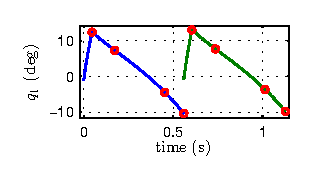
\includegraphics[width=.45\columnwidth]{7link_joint_q1}
  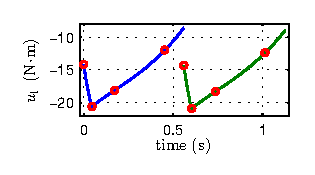
\includegraphics[width=.45\columnwidth]{7link_torque_u1}\\
  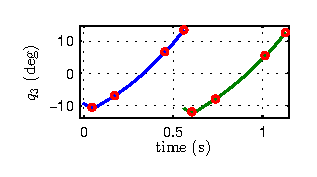
\includegraphics[width=.45\columnwidth]{7link_joint_q3}
  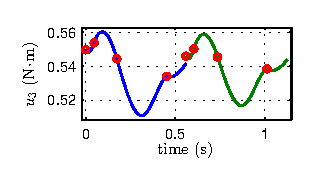
\includegraphics[width=.45\columnwidth]{7link_torque_u3}\\
  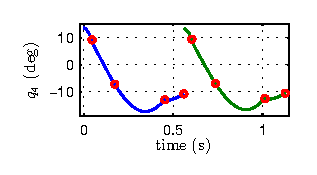
\includegraphics[width=.45\columnwidth]{7link_joint_q4}
  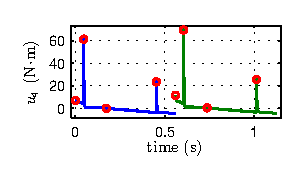
\includegraphics[width=.45\columnwidth]{7link_torque_u4}\\
  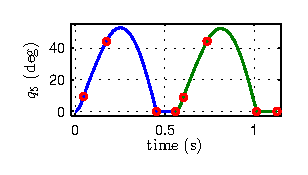
\includegraphics[width=.45\columnwidth]{7link_joint_q5}
  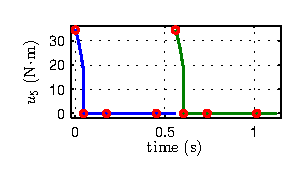
\includegraphics[width=.45\columnwidth]{7link_torque_u5}\\
  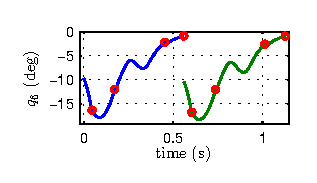
\includegraphics[width=.45\columnwidth]{7link_joint_q6}
  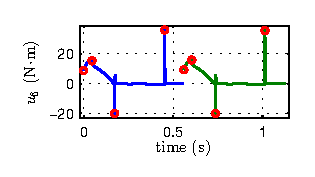
\includegraphics[width=.45\columnwidth]{7link_torque_u6}
  \caption[Joint and torque profiles for the seven-link biped gait over two
  steps.]{Joint and torque profiles for the seven-link biped gait over two
    steps.
  %
  The small circles represent the points where the discrete transitions occur.
  %
  }
  \label{fig:7link-noes-angles}
\end{figure}
%
The joint angles and torques resulting from this walking simulation are shown in
\figref{fig:7link-noes-angles}.
%
The stability of the gait can be examined by considering the codimension-one
\Poincare{} section $\Guard_{4}^{1}$, which is the guard of domain 4 (i.e., heel
strike) and involves switching legs.
%
To minimize the perturbations necessary to examine the \Poincare{} map, one can
perturb along a minimal set of bases that span the \Poincare{} map locally.

Non-holonomic constraints represent restrictions on the degrees of freedom of a
system and this shows up in a dropping of rank in the \Poincare{} map.
%
For this particular model, these minimal bases can be found by moving the fixed
frame to the fixed stance foot, then perturbing along angles $\qsn{3}$,
$\qsn{4}$, $\qsn{6}$ and angular velocities $\dqsn{1}$, $\dqsn{3}$, $\dqsn{4}$,
$\dqsn{6}$.
%
Because the knees are locked, $\qsn{2} = \dqsn{2} = \qsn{5} = \dqsn{5} = 0$ and
one can solve for $\qsn{1}$ such that the swing heel is on the ground.
%
Thus the \Poincare{} map for the orbit drops rank to seven.
%
Through optimization, the fixed point
\begin{align*}
  \qs^{*} &= (-.163, 0, .245, -.139, 0, -.003),\\
  \dqs^{*} &= (-.987, 0, 1.090, 1.068, 0, .067),
\end{align*}
is found.
%
A numerical approximation of a linearization of the Jacobian of the \Poincare{}
map in the seven minimnal bases yields eigenvalues with magnitudes $0.613$,
$0.169$, $0.056$, $\ldots$.
%
In general, eigenvalues with magnitudes below unity for discrete-time systems
indicate stability.
%
The \Poincare{} map for the simulated system is indeed stable thus implying
$(q^*, \dot q^*)$ is a fixed point of a stable periodic orbit which represents
the stable walking gait.

One could perform a similar analysis taking a different \Poincare{} section such
as the guard for knee lock.
%
This map has two bases more than the guard for heel strike as used above;
%
one may no longer solve for $\qsn{1}$ and $\dqsn{5}$ becomes arbitrary.
%
By taking this \Poincare{} section and performing analysis, one would find seven
non-zero eigenvalues for the reasons alluded to above.

\subsection{Simulation of Shaped System}

%\chapter{\uppercase{Literature Overview}}

\chapter{\uppercase{Conclusion}}

This thesis presented formal results for the method of energy shaping in
mechanical systems.
%
By taking advantage of conservation of energy, energy shaping seeks to improve
the performance characteristics of existing periodic behaviors.
%
Through the use of control Lyapunov functions, energy shaping acts on a
non-conservative system while guaranteeing that the periodic behaviors are not
destabilized.
%
This formal guarantee is a novel contribution that provides a significant
improvement over existing results which lacked this consideration.


As demonstrated, the methods, in some cases, may increase the domain of
attraction thereby increasing robust with respect to perturbations in initial
condition.
%
Simulation results also demonstrated that energy shaping appears to drive
systems to faster convergence.
%
The method was demonstrated on simple models to provide intuition and then on
more complex models to show versatility.
%
Simulations results and modeling for a multi-phase human gait for a biped with
feet were also provided to demonstrate energy shaping on a multi-domain hybrid
system.


When proving energy shaping, it was shown that a Lyapunov function exists
locally in the \Poincare{} map.
%
The exact form of this Lyapunov function is not known, but this begs the
question:
%
is it possible to explicitly construct a Lyapunov function, perhaps by guessing,
that could be used to analytically examine the domain of attraction?
%
In doing so, one would likely obtain a more complete understanding of robustness
properties.
%
Despite the lack of formal claims with respect to global properties, the local
stability properties are practically useful when using energy shaping as a
stabilizing controller in operating regions around the desired behavior.


In addition, this thesis does not make any claims about robustness with respect
to model uncertainties and measurement uncertainties.
%
It would be worthwhile to investigate model and measurement robustness in the
context of energy shaping and control Lyapunov functions in a wider context.
%
Such discussions are spread throughout the literature; see, e.g.,
\cite{Freeman1996}.
%
Open questions about the domain of attraction and robustness are pervasive
throughout the literature and are not unique to energy shaping;
%
however, their answers are left as the subject of future exploration.


When it comes to implementing formal algorithms on cyber-physical systems, there
is a number of pertinent considerations which determine the viability and
efficacy of a given controller.
%
A control algorithm which updates its commands too slowly will cause shaky
motion which in itself is indicative of imprecise control.
%
In addition, a slow loop rate means the system is slow to react to external
disturbances which makes it more difficult to reject them, thereby decreasing
the robustness of the system.
%
With bipeds this concern is of the utmost importance as the stability of a biped
depends on balancing the dynamic moment to keep the robot from toppling over.
%
Because feet tend to be narrow, stability in the coronal plane is a challenge
that frequently plagues roboticists.


In order to achieve smooth behavior in dynamic robots, it is therefore necessary
to have a relatively fast control loop and thus researchers seek to design
controllers which are computationally tractable.
%
Nonlinear controllers often give superior behavior in simulation but
their complexity renders them impractical for real-time implementation.
%
Oftentimes, controllers for robots are formulated as optimization problems which
use internal models to determine the appropriate control values.
%
The idea is to constrain the optimization problem to achieve the desired
behavior; typical formulations might take into consideration control of the zero
moment point to guarantee the system remains standing.


Considerations such as these generally lead to nonlinear optimization problems
which are problematic for a variety of reasons.
%
While a complex nonlinear formulation may represent a rigorous model of known
physical phenomena and may therefore match up very well with reality, the
computation cost may be prohibitive rendering such a formulation useful only in
simulation.
%
To overcome this problem, some researchers are turning quadratic programs for
which there exist efficient algorithms to quickly find solutions.
%
If one can formulate the constraints as a convex set, the solution can be found
easily and one can guarantee optimality whereas with nonlinear optimizations,
there is no guarantee on optimality over a given region.


The formulation presented in this paper is in the form of a quadratic program
whose optimization variables are joint torques and ground reaction wrenches.
%
This has great value because one can approximate friction cones with friction
pyramids (see \cite{Grizzle2014}) which are convex sets rendering friction
constraints amenable to the optimization problem.
%
Since the zero-moment point has a linear dependence on joint torques and ground
reaction wrench, this can also be factored into a quadratic program.
%
In addition, it is straightforward to impose bounds on torque.
%
Any of the above constraints or their combination may destroy the
feasibility of the optimization posed in \eqref{eq:es-qp}.
%
This potential issue with feasibility, however, can be addressed by relaxing the
constraints of the control Lyapunov function although this mitigates the formal
guarantee on stability.
%
Yet this leads to an interesting question:
%
is it possible to relax the constraints of a control Lyapunov function given in
\defref{def:lyap-func} and still guarantee stability?


A recent trend has found researchers formulating model predictive controllers
which attempt to determine control values by predicting their effect on the
behavior of the system over a future time window.
%
Energy shaping fits right into model predictive control (MPC) and could be used
to provide controllers which exhibit the benefits of energy shaping.
%
With MPC in particular, it is extremely important to have tractable controllers
as such controllers require multiple evaluations as the algorithm must integrate
forward to solve the relevant optimization problem.
%
The growth of computers is changing this paradigm but effective and robust
bipeds generally have fast control loops and this trend will likely continue for
some time.
%


Another area of interest which is seeing recent growth is precision control of
series elastic actuators (SEA), particularly in systems such as bipeds which
experience a wide range of dynamic forces.
%
While control of SEA is more challenging than control of traditional actuators,
the potential benefits make it an important phenomenon to understand.
%
The addition of series compliance not only allows for force sensing at joints
but also for energy storage which can be utilized through design methods like
energy shaping.
%
Force sensing leads to additional possibilities such as online system
identification which can provide vital information about the mass distribution
of a robot.
%
By improving the internal model, model-based methods such as energy shaping see
improved robustness; this is particularly helpful for MPC.
%

The models studied in this paper involve traditional actuation schemes rather
than SEA.
%
This decision choice was instrumental in achieving formal results but it is
important to recognize that SEA is seeing increasing use in robot design and
this trend is likely to continue.
%
In order to handle SEA formally, new control schemes have to be formulated which
take the compliance into account.
%
This naturally begs the question:
%
Can energy shaping be formulated in a tractable way on systems with SEA?
%
The answer to this question is not likely be straightforward as SEA requires the
addition of double integrators in the model which would change the nature of an
optimization problem like \eqref{eq:es-qp}.



% fix spacing in bibliography, if any...
%%%%%%%%%%%%%%%%%%%%%%%%%%%%%%%%%%%%%%%%%%%%%%%%%%%%%%%%%%%%%
\let\oldbibitem\bibitem
\renewcommand{\bibitem}{\setlength{\itemsep}{0pt}\oldbibitem}
%%%%%%%%%%%%%%%%%%%%%%%%%%%%%%%%%%%%%%%%%%%%%%%%%%%%%%%%%%%%%%%
%%%%%%%%%%%%%%%%%%%%%%%%%%%%%%%%%%%%%%%%%%%%%%%%%%%
%
%  New template code for TAMU Theses and Dissertations starting Fall 2012.  
%  For more info about this template or the 
%  TAMU LaTeX User's Group, see http://www.howdy.me/.
%
%  Author: Wendy Lynn Turner 
%	 Version 1.0 
%  Last updated 8/5/2012
%
%%%%%%%%%%%%%%%%%%%%%%%%%%%%%%%%%%%%%%%%%%%%%%%%%%%


%%%%%%%%%%%%%%%%%%%%%%%%%%%%%%%%%%%%%%%%%%%%%%%%%%%%%%%%%%%%%%%%%%%%%%
%%                           REFERENCES 
%%%%%%%%%%%%%%%%%%%%%%%%%%%%%%%%%%%%%%%%%%%%%%%%%%%%%%%%%%%%%%%%%%%%%

\phantomsection
\addcontentsline{toc}{chapter}{REFERENCES}

\renewcommand{\bibname}{{\normalsize\rm REFERENCES}}

\makeatletter
\renewcommand\@biblabel[1]{[#1]}
\makeatother

\bibliographystyle{IEEEtranS}
\bibliography{myrefs}

%%%%%%%%%%%%%%%%%%%%%%%%%%%%%%%%%%%%%%%%%%%%%%%%%%%%
%
%  New template code for TAMU Theses and Dissertations starting Fall 2012.  
%  For more info about this template or the 
%  TAMU LaTeX User's Group, see http://www.howdy.me/.
%
%  Author: Wendy Lynn Turner 
%	 Version 1.0 
%  Last updated 8/5/2012
%
%%%%%%%%%%%%%%%%%%%%%%%%%%%%%%%%%%%%%%%%%%%%%%%%%%%

\begin{appendices}
\titleformat{\chapter}{\centering\normalsize}{APPENDIX \thechapter}{0em}{\vskip .5\baselineskip\centering}
\renewcommand{\appendixname}{APPENDIX}

%%%%%%%%%%%%%%%%%%%%%%%%%%%%%%%%%%%%%%%%%%%%%%%%%%%
%
%  New template code for TAMU Theses and Dissertations starting Fall 2012.  
%  For more info about this template or the 
%  TAMU LaTeX User's Group, see http://www.howdy.me/.
%
%  Author: Wendy Lynn Turner 
%	 Version 1.0 
%  Last updated 8/5/2012
%
%%%%%%%%%%%%%%%%%%%%%%%%%%%%%%%%%%%%%%%%%%%%%%%%%%%

%%%%%%%%%%%%%%%%%%%%%%%%%%%%%%%%%%%%%%%%%%%%%%%%%%%%%%%%%%%%%%%%%%%%%%
%%                           APPENDIX A 
%%%%%%%%%%%%%%%%%%%%%%%%%%%%%%%%%%%%%%%%%%%%%%%%%%%%%%%%%%%%%%%%%%%%%

\phantomsection

\chapter{\uppercase{First Appendix}}

Text for the Appendix follows.

\begin{figure}[H]
\centering
\includegraphics[scale=.50]{figures/Penguins.jpg}
\caption{TAMU figure}
\label{fig:tamu-fig5}
\end{figure}

%%%%%%%%%%%%%%%%%%%%%%%%%%%%%%%%%%%%%%%%%%%%%%%%%%%
%
%  New template code for TAMU Theses and Dissertations starting Fall 2012.  
%  For more info about this template or the 
%  TAMU LaTeX User's Group, see http://www.howdy.me/.
%
%  Author: Wendy Lynn Turner 
%	 Version 1.0 
%  Last updated 8/5/2012
%
%%%%%%%%%%%%%%%%%%%%%%%%%%%%%%%%%%%%%%%%%%%%%%%%%%%

%%%%%%%%%%%%%%%%%%%%%%%%%%%%%%%%%%%%%%%%%%%%%%%%%%%%%%%%%%%%%%%%%%%%%%
%%                           APPENDIX B
%%%%%%%%%%%%%%%%%%%%%%%%%%%%%%%%%%%%%%%%%%%%%%%%%%%%%%%%%%%%%%%%%%%%%

\chapter{\uppercase {Second Appendix with a longer title - much longer in fact}}

Text for the Appendix follows.

\begin{figure}[H]
\centering
\includegraphics[scale=.50]{figures/Penguins.jpg}
\caption{TAMU figure}
\label{fig:tamu-fig6}
\end{figure}

\section{Appendix Section}


\pagebreak{}


\end{appendices}


\end{document}
